%\documentclass[11pt,twoside,openright,letterpaper]{book}
\documentclass[11pt,twoside,openright,letterpaper]{memoir}
\setsecnumdepth{subsection} % include numbering on subsections

\usepackage{titling}
\usepackage{helvet} % Use Helvetica font.
\renewcommand{\familydefault}{\sfdefault}
\usepackage{setspace}
\usepackage{tabularx}
\usepackage[super,comma,sort&compress]{natbib}
% switch bibliography numbering to 1. from [1] :
\makeatletter \renewcommand\@biblabel[1]{#1.} \makeatother
\usepackage{siunitx} % for math formatting
\usepackage{newtxtext,newtxmath} % formats numbers in math mode to consistent font

\usepackage{hyperref} % allow urls
\hypersetup{
    pdfauthor={CLCampbell},
%    pdfsubject={Some subject},
    pdftitle={},
%    pdfkeywords={LaTeX, PDF, hyperlinks}.
    citebordercolor = {1 1 1}, % no box around citations
    %,pdfborder = {0 0 1} % visible box around hyperlinks.
    %,pdfborderstyle={/S/U/W 1}
    colorlinks,
    citecolor=black,
    filecolor=black,
    linkcolor=black,
    urlcolor=black % blue
}

% Use 1/2-inch margins.
\usepackage[margin=1in,lmargin=1.5in]{geometry}

\title{Deep characterization of meiotic crossover and gene conversion}

\author{Christopher L Campbell}
%Albert Einstein College of Medicine}

\makeatletter\let\Title\@title\makeatother
\makeatletter\let\Author\@author\makeatother

% \newenvironment{abstract}%
% {\cleardoublepage\null \vfill\begin{center}%
% \bfseries \abstractname \end{center}}%
%     {\vfill\null}

\usepackage{tocbibind} % include toc within toc
\usepackage{titlesec}

\newenvironment{titemize} {
	\begin{itemize}
	  \setlength{\itemsep}{0cm}%
	  \setlength{\parskip}{0cm}%
} {\end{itemize}}

\newenvironment{tenumerate} {
	\begin{enumerate}
	  \setlength{\itemsep}{0cm}%
	  \setlength{\parskip}{0cm}%
} {\end{enumerate}}

%%%%%%%%%%%%%%%%%%%%%%%%%%%%%%
%%%%%%%%%%%%%%%%%%%%%%%%%%%%%%
\begin{document}
%%%%%%%%%%%%%%%%%%%%%%%%%%%%%%
%%%%%%%%%%%%%%%%%%%%%%%%%%%%%%

% \setcounter{tocdepth}{5}
% \setcounter{page}{1}

\frontmatter

%\begin{titlepage}
\begin{titlingpage}
\begin{center}
    \vspace*{1cm}
    \Large{ \textbf{\Title} } \\
    \vspace{1.5cm}
    \normalsize
    \Author \\ \vspace{2cm}
    \begin{tabularx}{\textwidth}{@{}X@{}X@{}}
        \begin{minipage}[t]{\linewidth}
            \textbf{Candidate:} \\ 
            %\vspace{1.5cm} \hrule\smallskip Signature
            \vspace{1.5cm} \hrule width 0.9\textwidth \smallskip Signature
            %\vspace{1.5cm} \noindent\rule{0.9\textwidth}{0.4pt}
        \end{minipage}
        & \\
        \begin{minipage}[t]{\linewidth}
            \vspace{1cm}
            \textbf{Thesis Advisor:} \\ 
            \vspace{1.5cm} \hrule width 0.9\textwidth \smallskip Signature
            \begin{flushleft}
                Adam Auton, D.Phil. \\
                \small \smallskip
                Assistant Professor, Department of Genetics \\
                Assistant Professor, Department of Epidemiology \& Population Health \\
            \end{flushleft}
        \end{minipage}
        \vspace{1cm}
        &
        \begin{minipage}[t]{\linewidth}
            \vspace{1cm}
            \textbf{Co-advisor:} \\ 
            \vspace{1.5cm} \hrule width 0.9\textwidth \smallskip Signature
            \begin{flushleft}
                Bernice E. Morrow, Ph.D. \\
                \small \smallskip
                Professor, Department of Genetics \\
                Professor, Department of Obstetrics \& Gynecology and Women's Health \\
                Professor, Department of Pediatrics (Cardiology) \\
                Sidney L. and Miriam K. Olson Chair in Cardiology \\
                Director, Division of Translational Genetics, Department of Genetics \\
            \end{flushleft}
        \end{minipage}\\
    \end{tabularx}
%%%
\vfill
Submitted in partial fulfillment of the requirements for the Degree of Doctor of
Philosophy in the Graduate Division of Medical Sciences.
\vspace{0.5cm}
\\ Albert Einstein College of Medicine
\\ Yeshiva University
\\ New York
\\ December 2016
\end{center}
%\end{titlepage}
\end{titlingpage}
%\newpage
\setcounter{page}{1}


%%%%%%%%%%%%%%%%%%%%%%%%%%%%%%
%%%%%%%%%%%%%%%%%%%%%%%%%%%%%%
\chapter{Abstract}
%%%%%%%%%%%%%%%%%%%%%%%%%%%%%%
%%%%%%%%%%%%%%%%%%%%%%%%%%%%%%
% Abstract: The abstract of the Dissertation is to include: a hypothesis, the procedures followed, the
% significant results and the general conclusions. The abstract is to be presented on a separate page
% headed with the word ABSTRACT in capital letters centered on the page. On the next line is the
% title of the Dissertation. The following line is the full name of the student. The length of the
% abstract must not exceed 600 words. (Please note the separate instructions for the 350 word
% microfilm copy abstract described in the first section of this manual.)
\thispagestyle{plain}
\begin{centering} ABSTRACT \\ %\end{centering}
\noindent\Title \\
\Author \\
\end{centering}




%%%%%%%%%%%%%%%%%%%%%%%%%%%%%%
%%%%%%%%%%%%%%%%%%%%%%%%%%%%%%
\chapter{Acknowledgements}
%%%%%%%%%%%%%%%%%%%%%%%%%%%%%%
%%%%%%%%%%%%%%%%%%%%%%%%%%%%%%
% The Training Program in Cellular and Molecular Biology and Genetics, T32 GM007491.


\tableofcontents
\listoffigures
\listoftables

%%%%%%%%%%%%%%%%%%%%%%%%%%%%%%%%%%%%%%%%%%%%%%%%%%
\mainmatter
%%%%%%%%%%%%%%%%%%%%%%%%%%%%%%%%%%%%%%%%%%%%%%%%%%

%%%%%%%%%%%%%%%%%%%%%%%%%%%%%%
\chapter{Introduction}
%%%%%%%%%%%%%%%%%%%%
% Introduction chapter

%%%%%%%%%%%%%%%%%%%%%%%%%%%%%%%%%%%%%%%%
%%%%%%%%%%%%%%%%%%%%%%%%%%%%%%%%%%%%%%%%
\section{An overview of meiotic recombination}
%%%%%%%%%%%%%%%%%%%%%%%%%%%%%%%%%%%%%%%%
%%%%%%%%%%%%%%%%%%%%%%%%%%%%%%%%%%%%%%%%

Meiosis occurs in all sexually reproducing organisms, and is essential to the generation of gametes.
Recombination plays a key role in this process, facilitating the pairing and alignment of chromosomes, while the exchange of genetic material has important implications in inheritance, natural selection, and evolution.

\afterpage{
\begin{figure}[P]
    \begin{center}
    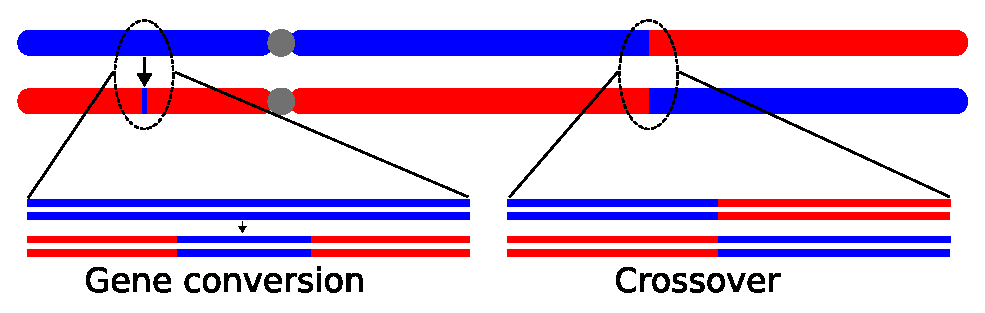
\includegraphics[width=\textwidth]{introduction/figs/outcome_CO-GC}
    \end{center}
    \vspace{-10pt}
    \captionTitle{\textbf{Recombination produces crossover and gene conversion.}}{ 
        Recombination is initiated by DNA double strand breaks that resolve into one of two possible outcomes.
        Crossover (shown at right) is the large-scale, reciprocal exchange of genetic material between two chromosomes around the break point.
        Gene conversion (or non-crossover, shown at left) is the one-way transfer of small amounts of DNA from one chromosome to the other during the repair of the break.
   \label{fig:introOutcomes}}
\end{figure}
\clearpage}


%%%%%%%%%%%%%%%%%%%%%%%%%%%%%%%%%%%%%%%%
\subsection{The biology of meiotic recombination}
%%%%%%%%%%%%%%%%%%%%%%%%%%%%%%%%%%%%%%%%

Prior to meiosis, a diploid cell contains pairs of homologous chromosomes, one of the pair inherited from the father, the other from the mother.
This diploid DNA is replicated just prior to the cell entering the meiotic cycle, in premeiotic S-phase\cite{Bell2002} to generate exact copies of each pair of chromosomes, referred to as sister chromatids.
Meiosis consists of two stages; recombination occurs in the first, meiosis I, while meiosis II sees sister chromatids separate into their respective daughter cells.
Meiosis I is the most complex and lengthy stage, with chromosome pairing, synapsis, and recombination all occurring in succession within prophase I, which is  divided into several sub-stages.

In leptotene (derived from Greek meaning ``thin threads''), changes in chromatin cause the newly replicated chromosomes to form thin individual strands.
Here, the synaptonemal complex (SC), a protein structure that will bind the sister chromatids and their homologues into a tetrad begins to assemble.
The SC consists of a scaffold of proteins that first forms with axial elements that associate with the already paired sister chromatids, solidifying their association.

In the zygotene phase (``paired threads''), pairing between the unraveled DNA begins to occur at regions of homology in a process known as synapsis.
Homologous chromosomes connect to to the SC by transverse filaments, drawing them into the SC structure in a progressive zipper-like mechanism, completing synapsis\cite{Yang2009}.
DNA DSBs occur at this stage (*).

By the pachytene stage (``thick threads''), synapsis, and the SC assembly are fully complete, and the pairs of homologous chromosomes bound within the SC are referred to as a tetrad or bivalent.
Recombination occurs here, mediated by the structure of the SC.
A subset of the DSBs are processed as crossovers, at locations called chiasmata.
The remaining DSBs are repaired through a different pathway, as non-crossovers (gene conversions).

In the diplotene stage (``two threads''), the SC is disassembled, allowing the tetrad to relax slightly.
The homologous chromosomes are still held together at chiasmata locations.

In the final substage of prophase I, diakinesis (``moving through''), the chromosomes condense into visible threads, while the cellular machinery begins to prepare for cell division.
The remaining step of meiosis I are metaphase I, and anaphase I.
Chiasmata, holding the chromosomes together as crossover points are cut, allowing the homologous chromosomes to segregate to their respective cellular poles.

Meiosis II is procedurally similar to mitosis, with different results.
Here, the separation of sister chromatids occurs, producing four haploid gametes.




The recombination process is begun by programmed double strand breaks (DSBs) in the DNA, catalyzed by the protein SPO11, which has a similar function to DNA topoisomerases\cite{DeMassy2013}.
There are two isoforms of \textit{Spo11} in humans, and mice, and a recent study in mice suggests that they may have differing functions, with \textit{Spo11$\beta$} being expressed earlier in meiosis, coinciding with most DSBs occurring on the autosomes.
Male mice with only \textit{Spo11$\beta$} had meiotic defects, with the majority of spermatocytes failing to recombine in the pseudoautosomal region (PAR).
Following this, \textit{Spo11$\alpha$} was found to be expressed later in meiosis, and coincided with DSBs located within the sex chromosomes, including the PAR\cite{Kauppi2011,DeMassy2013}.
This evidence indicates that the initiation of DSBs is a complex, multi-stage process, with autosomal DNA process earlier than DNA from the sex chromosomes.




\paragraph{Non-disjunction and the role of recombination.}
In humans, an estimated 30\% of fertilized eggs have aneuploid chromosomes\cite{Hassold2001}, and evidence suggests that meiotic errors are responsible in many cases.
Non-disjunction, the abnormal segregation of chromosomes, can occur at either of the two cell divisions in meiosis.
Meiosis II non-disjunction typically results from a failure of the sister chromatids to separate.
Meiosis I non-disjunction is thought to involve recombination, either in a failure to resolve chiasmata, or a lack of chiasmata entirely.

A reduced recombination rate has been observed in human genetic maps generated from viable meiosis I aneuploidies (15, 16, 18, 21, XXX, XXY)\cite{Hassold2001,Lynn2004}.
This indicates that recombination rate must remain above a certain level to prevent non-disjunction.
This is supported by the finding that many trisomies involve achiasmate chromosomes, in which recombination is absent in that chromosome(*).

This supports the idea that chiasmata, which serve to tether homolgous chromosomes together after the dissolution of the SC, and through the first, provide a crucial tension that serves to inhibit non-disjunction.
Research suggests that there is a requirement of one chiasma per chromosome to prevent non-disjunction, but that there may be a backup mechanism to enable chromosomes to properly segregate even without any chiamata\cite{Fledel-Alon2009}.



%%%%%%%%%%%%%%%%%%%%%%%%%%%%%%%%%%%%%%%%
\subsection{Timing of meiotic events}
%%%%%%%%%%%%%%%%%%%%%%%%%%%%%%%%%%%%%%%%

%Human:
The fundamental steps of meiosis are the same in males and females, but the timing of these events, both prior and during, differs significantly between the sexes\cite{Lynn2004}, and even between species.
In humans, male meiosis begins at puberty and continues in a cycle that lasts throughout the lifespan.
As male meiosis is continually occurring, the precursor cells undergo a minimum of 30 divisions prior to entering meiosis, and this number continues to rise with age.
A 15 year old male is estimated to be 35 germ-cell divisions, with this number rising to 380 at age 30, and 840 by age 50\cite{Crow2000a}.

Females have 22 cell divisions prior to meiotic entry, and one during, for a total of 23 divisions\cite{Crow2000a}, and this number is fixed for all oocytes.
In females, meiosis begins prenatally, and oocytes progress through the diplotene stage of prophase I before undergoing an arrest period\cite{Hassold2001,Crow2000a}.
This arrest is called the dictyotene stage, or dictyate arrest, and meiosis is frozen at the point the chromosomes have fully synapsed and chiasmata have formed (Figure \ref{fig:introTiming}).
This arrest period ends only upon ovulation, and thus meiosis can be potentially very lengthy, taking one to five decades to complete.
Additionally, while each male meiosis produces four haploid sperm products, female meiosis yields one haploid oocyte contain the majority of the cytoplasm, the remaining meiosis I and II division products produce polar bodies, which contain DNA but typically apoptose\cite{Schmerler2011}.

Male progenitor cells undergo potentially many more mitotic divisions prior meiotic entry.
As the number of mitioc proliferations increases in males, so does the number of mutations accumulated through DNA replication errors.
A recent study using a chimpanzee pedigree estimated that the number of mutations rises linearly with the father's age, with approximately three additional mutations accumulating per year\cite{Venn2014}.
This contributes to a paternal age effect, with mutations accumulating on the male germ line with increasing age.

Dog meiosis differs from that of humans in some key respects.
Meiosis in female dogs begins later, starting in the neonatal period\cite{Freixa1987}.
The meiotic arrest occurs at the same dictyotene stage in both species, but is shorter in dogs, given the later onset of meiosis in dogs as well as a reduced lifespan.
In addition, while meiosis exits the arrest period prior to ovulation in humans, dogs ovulate immature, primary oocytes, which only mature to fertility 48-60 hours after ovulation\cite{Tsutsui1989,Chastant-Maillard2011}.

\afterpage{
\begin{figure}[P]
    \begin{center}
    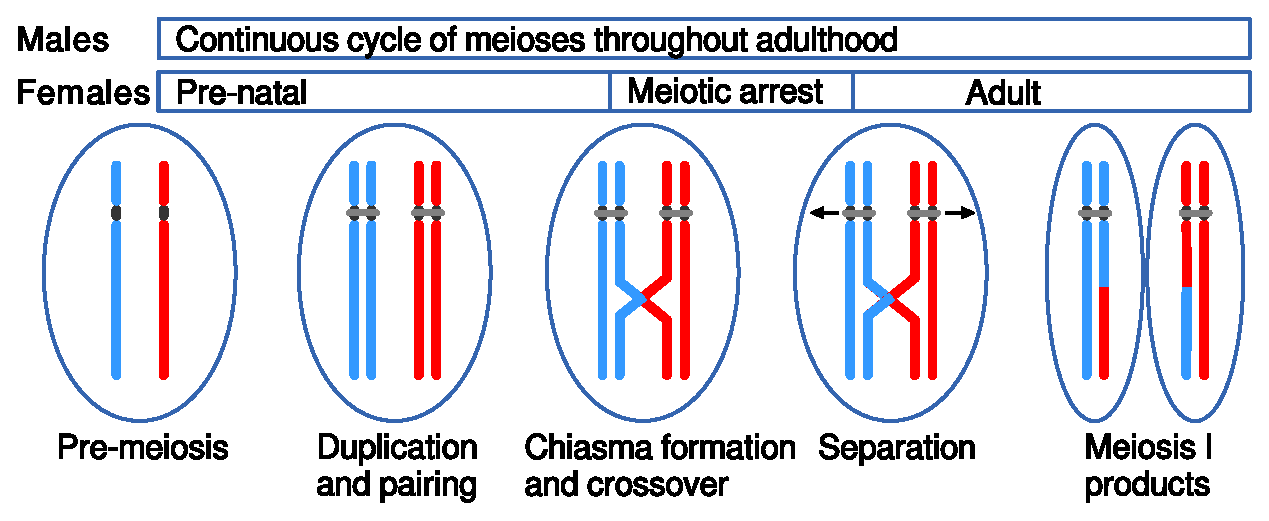
\includegraphics[width=\textwidth]{introduction/figs/meioticTiming}
    \end{center}
    \vspace{-10pt}
    \captionTitle{\textbf{Timing of meiosis I events in humans.}}{ 
        Males exhibit a continuous wave of meioses throughout adulthood.
        In females, meiosis begins before birth and enters an arrest period that can last decades before completion.
   \label{fig:introTiming}}
\end{figure}
\clearpage}

Several biological possibilities have been proposed to explain what happens to oocytes during meiotic arrest.
Polani1991, Rowsey2014: Production line hyp.
Polani: production line holds true for mice



%%%%%%%%%%%%%%%%%%%%%%%%%%%%%%%%%%%%%%%%
%%%%%%%%%%%%%%%%%%%%%%%%%%%%%%%%%%%%%%%%
\section{Historical overview of meiotic recombination}
%%%%%%%%%%%%%%%%%%%%%%%%%%%%%%%%%%%%%%%%
%%%%%%%%%%%%%%%%%%%%%%%%%%%%%%%%%%%%%%%%

% Brief historical review of meiotic recombination, pre Human Genome Project.
Recombination can be observed in a number of ways, and its discovery came decades prior to the discovery of the structure of DNA.
Thomas Hunt Morgan first observed the separation of linked traits while studying Drosophila in 1911\cite{Morgan1911}, and proposed the theory of crossing over between chromosomes.
In addition he suggested that the recombination rate could increase with the distance between factors.
Morgan's student, Alfred Henry Sturtevant, quantified this change in rate over physical distance into ``map distance,'' using this concept to construct the first genetic map.
This map represented the order of, and crossover rates between, genes on the X chromosome in Drosophila\cite{Sturtevant1913}.
In addition, Sturtevant observed that one crossover tended to inhibit the placement of a second nearby, an early description of interference.
A later study by Harriet Creighton and Barbara McClintock in corn (\textit{Zea mays}) in 1931 demonstrated that recombination between genes was tied to an exchange of chromosomal segments\cite{Creighton1931}.

Tracing the inheritance of markers from one generation to the next within a family pedigree provided the first genome-wide measurement of recombination across the human genome, prior to the completion of the Human Genome Project.
Early studies used restriction fragment length polymorphism (RFLP) probes to identify specific loci within the genome, and determine if they are linked.
An early study described the use of RFLPs to generate a linkage map of recombination in the human genome\cite{Botstein1980}.
Further linkage studies increased the marker density across the genome by using microsatellite, short tandem repeat polymorphisms (STRPs) and other approaches to capturing genetic variation\cite{Morton1991,Matise1994,Dib1996}.
The Marshfield map, generated in 1998 by \citet{Broman1998}, was an important step in characterizing recombination on a genome-wide basis.

With the completion of the Human Genome Project and the publication of the draft sequence of the human genome\cite{Venter2001,Lander2001}, human genetic variation has become increasingly well characterized, and a number of technologies have sprung up to make genome-wide ascertainment of variation routine.
Currently, microarray technology provides a well-balanced approach for determining genome-wide coverage of genetic variation.
These arrays target a pre-selected panel of hundreds of thousands to millions of single-nucleotide polymorphisms (SNPs) across every chromosome for a reasonable cost.

%%%%%%%%%%%%%%%%%%%%%%%%%%%%%%
\section{Methods for studying recombination}
%%%%%%%%%%%%%%%%%%%%%%%%%%%%%%

Genome-wide methods have the primary goal of creating a genetic map of the frequency of recombination as a function of physical distance across each chromosome.
In contrast, several other methods are limited in scope, and reveal information about specific loci.
With each method, the detection of recombination is made difficult by the fact that crossovers are rare -- only 20-50 are expected to occur in each meiosis.

% brief introduction to these before describing in detail in "description of approach"

\subsection{Pedigree analysis}

Tracking the transmission of alleles from one generation to the next within known pedigrees provided the first data on recombination in early linkage studies, and pedigree analyses are still in use today.
It is interesting to note that for a pedigree analysis, 
while whole-genome sequencing technology allows the discovery of a higher density of markers across the genome, its use is not typically worth the higher cost.
A higher variant coverage will help to narrow the region of uncertainty surrounding a particular crossover, but it will most likely not assist in the detection of additional crossovers in a single meiosis.

Regardless of the method used for obtaining markers, the principle of detecting recombination in a pedigree remains.
Crossovers can be identified by tracing the allele transmissions from parent to child.
Figure \ref{fig:introPedfig} provides a simple visual example, showing a family quartet.
The father in this pedigree has two informative SNPs producing haplotypes 1-1 and 0-0, while the mother is homozygous at both sites.
The male child has a 1-0 haplotype, and therefore must have inherited a recombinant haplotype from his mother.
We can identify here a crossover event and localize that event to an interval flanked by two informative genetic variants.
This region of uncertainty can vary in size and depends on the spacing and genotypes of polymorphic variants within the genome.
Beyond this intuitive example, the problem of determining the parental phase of a recombinant chromosome has been addressed in a number of methods.
%
\afterpage{
\begin{figure}[p]
    \begin{center}
    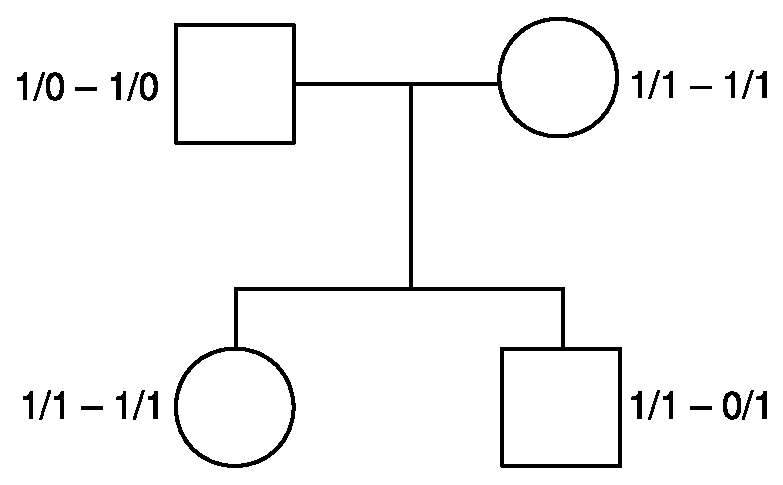
\includegraphics[width=0.75\textwidth]{introduction/figs/pedigree-genotype} \vspace{1cm} \\
    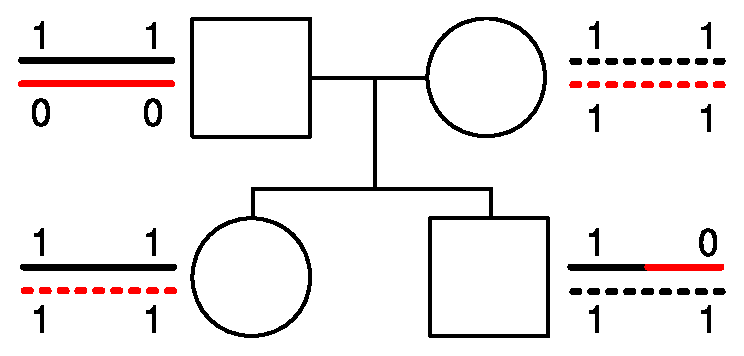
\includegraphics[width=0.8\textwidth]{introduction/figs/pedigree-haplotype}
\end{center}
    \vspace{-10pt}
    \captionTitle{\textbf{Allelic transmission in a family quartet.}}{ 
        The top panel outlines a simple pedigree in which only genotype information is known.
        The bottom panel shows a pedigree for which phase-known haplotype information is known.
        Here, all chromosomes (lines next to each individual) are transmitted in the absence of recombination except for in the male child.  Here there was a recombination event in the father to generate the recombinant chromosome (black/red)
   \label{fig:introPedfig}}
\end{figure}
\clearpage}


\subsection{Linkage disequilibrium approach}

Another powerful method is to use population genetic data to study recombination by inference.
These data can be gathered by genotyping samples of genetic data from unrelated individuals on a microarray or by whole-genome sequencing.

The inference of recombination in such a dataset relies on the quantification of levels of linkage disequilibrium (LD) within the samples, a measurement of linkage between loci.
For example, when alleles at one locus are inherited completely independently of alleles at another locus they are considered to be in linkage equilibrium.
However many alleles exhibit a non-random association, and individuals of the same species tend to share haplotype segments that reflect a shared evolutionary history.
When two alleles on an ancestral haplotype are inherited together they are considered linked, and are not independent of each other.
These alleles exhibit evidence of linkage disequilibrium, a deviation from the assumption of random assortment of alleles.

LD is measured in a pairwise fashion, considering allele frequencies at each pair of markers in the genome.


From measurements of LD within a number of unrelated samples, methods based on coalescent theory have been developed to estimate the recombination rate\cite{Auton2012}.
In software such as LDhat\cite{Mcvean2004,Auton2007,Auton2014}, the population-scale recombination rate, $\rho$, is estimated from the data, and the per-generation recombination rate can be calculated by the relationship
$\rho = 4 N_e r$
where $N_e$ represents the effective population size.
These methods are quite powerful and have produced high-quality estimates of recombination in humans\cite{hapmap2007}, however, they are subject to limitations.
First, that this method requires the knowledge of the genealogical history of a sample, which is unknown, and thus relies on an often simplistic approximation.
Second, these maps by their nature generate sex-averaged data only, since recombination events that are inferred have occurred over the course of potentially thousands of generations.


\subsection{Molecular assays}

A number of molecular assays have been developed for studying recombination.
Most, however are limited to small regions of the genome, and are more effective in males.

\subsubsection{Sperm cell assays}

Sperm typing is one method of identifying both gene conversion and crossover events.
Sperm typing was first used in 1989 to study crossing over in humans\cite{Cui1989}, and uses
allele-specific polymerase chain reaction (PCR) to identify recombination events at a given locus.
In this method, DNA is extracted from multiple haploid sperm cells from a single donor and subject to PCR.
A common reverse primer is used in conjunction with two different allele-specific forward primers, which correspond to polymorphic site in the diploid genome, and are designed to produce different amplicon sizes depending on the matching nucleotide.
Analysis of the PCR products from many sperm cells can reveal the phase of the donor individual, and the recombinant status of each sperm cell.
% \cite{Jeffreys1998,Jeffreys2000,Jeffreys2004}. % first, second(TAP2), review

Sperm typing has been used to produce high-quality data from a number of loci throughout the genome.
One of the first major findings to come out of sperm typing was the characterization of a recombination hotspot in the human major histocompatability complex (MHC), first within one gene, \textit{TAP2}\cite{Jeffreys2000}, then expanded to cover a wider 216 kb region of the MHC\cite{Jeffreys2001}.
All six hotspots found within the region of the MHC were found to be tightly correlated to regions in which LD broke down, providing molecular evidence that recombination hotpots have severe effects on LD patterns.


Jeffreys2009: rise/fall

Berg2010

\citet{Lu2012}
\citet{Wang2012}


\subsubsection{Single oocytes.}
Recent studies have provided much needed insight into recombination in single oocytes through novel methods.
\citet{Hou2013} conducted an analysis in human oocytes, providing at the same time a potential new method for applying next generation sequencing methods to the screening for various genetic disorders with in vitro fertilization (IVF) techniques.
Here, the researchers extracted and fertilized a total of 70 oocytes from 8 Asian female donors, collecting the first and second polar bodies, as well as the male and female pronucleus from the fertilized egg.
This complete collection of data from female oogenesis and fertilization enabled haplotype phasing and crossover calls
Most intriguingly, this enabled the generation of personal genetic maps for each donor, allowing the researchers to address the question of how recombination varies on an individual basis.
This data allows the observation of all four members of the tetrad bundle, both sister chromatids and their homologues, something usually missed by inferential studies of recombination.


Using a similar approach, recovering genetic materiel from the first and second polar bodies and oocyte, \citet{Ottolini2015} were able to observe all four products of female recombination.
The researchers generate ``MeioMaps,'' providing valuable information on how meiosis proceeds on an individual level.



\subsubsection{Recombination initiation maps}
Additional methods have been developed to identify double strand breaks within a individual cells undergoing meiotic recombination.
\citet{Pratto2014} utilized chromatin immunoprecipitation coupled with sequencing to identify DSBs associatated with the strand-exchange protein DMC1 to generate DSB maps in four unrelated human males.
This method identifies the majority of DSBs within the meiotic cell, only a fraction of which will be resolved as crossovers that could be identified via genotyping methods, the remainder ending up as non-crossover gene conversions.
The researchers found the DSB cluster into hotspots, of which 51\% overlapped with the LD crossover hotspots\cite{hapmap2007}, and 80\% of DSB hotspots overlapped regions with elevated recombination rate.
In addition, the DSB locations were largely tied to the specific PRDM9 allele for each particular individual.
PRDM9$_\text{A}$ and PRDM$_\text{B}$ alleles appear to specify similar DSB hotspots, while PRDM9$_\text{C}$ has a separate specificity.
PRDM9 heterozygosity also affects hotspot strength.


% \section{Current ``gold standard'' maps (Hapmap2 LD map, deCODE pedigree map).}
\section{Genetic maps of recombination.}

\subsection{Marshfield map}
The Marshfield map, generated by \citet{Broman1998} in 1998, was the first genetic map of the human genome at a resolution high enough to make inferences on the recombination properties in humans, using $>$8000 short tandem repeat polymorphsims (STRPs) in 188 meioses.
Here, estimates of the genome wide map lengths, inferences on individual variation, and sex differences in recombination were highlighted.
The ratio of female to male autosomal map length was estimated at 1.56, indicating that the recombination rate in females is substantially higher than males.
This ratio has proved stable over a number of studies in the intervening years (summarized in Table \ref{tab:introHeterochiasmy}).
Analysis of this this ratio as a function of chromosome position revealed that male recombination tends to be highest in the telomeres, while females had a higher ratio towards the centromeres.
This study provided valuable insight into sex dimporphism in recombination

\subsection{deCODE maps}
Another major stride in pedigree-based genetic maps came from deCODE genetics, an Icelandic pharmaceutical company that used their database of genealogical and genetic data on many Icelandic families to infer recombination, producing many high quality studies.
The first was in 2002, where 146 families, comprising 1257 meioses, were genotyped using 5136 microsatellite markers\cite{Kong2002}.
This data, in conjunction with the draft sequence of the human genome\cite{Venter2001,Lander2001} was used to improve the marker order and their placement within the reference sequence.
The genetic map generated from this study confirmed much found by \citet{Broman1998} in terms of sex dimorphism in recombination, and further characterized fine scale variation between the chromosomes.
One particular finding was that of recombination ``jungles,'' regions of high crossover rate that clustered towards the telomeres.
In addition, recombination rate was found to correlate with GC content, CpG motif occurrance, and tracts of poly(A)/poly(T), together explaining $\sim$37\% of variation.

In 2010, using genome wide SNP data on x meioses, deCODE genetics published an updated sex-specific recombination map\cite{Kong2010}.
Instead of a typical pedigree-based recombination study, \citet{Kong2010} leverage the high degree of relatedness within the Icelandic population to infer phase and parent-of-origin in 20,217 individuals typed on microarrays assaying $>$289,000 autosomal SNPs.
Here, phase is determined for parent-child pairs by taking into account haplotype blocks that are shared with other individuals within the population to determine the parent-of-origin for a particular block.
Crossovers are called when a segment of a child's haplotype is inferred to move between maternal and paternal origin.
This enables recombination be called in 15,257 parent-offspring pairs.
%%%
One effect of this parent-child phasing approach is that inference of recombination events near the telomeres is difficult, and \citet{Kong2010} omit the most distal 5 Mb for each chromosome.
The omission of the telomeric regions, where male recombination is higher, contributes to the inflation of the female:male map length ratio seen in Table \ref{tab:introHeterochiasmy}) at 1.78 in this study, however much more likely to be closer to the consensus ratio of around 1.56.
Since its release in 2010 the deCODE genetic map has proven quite valuable as a high quality sex-specific map of recombination in the human genome.


\paragraph{Other pedigree studies.}
A study in 2008 employed a pedigree analysis of individuals from the Hutterite population, all of European descent\cite{Coop2008}.
This was the first study to use genome-wide high-density SNP arrays (in this case the Affymetrix GeneChip Mapping 500k array) to study recombination.
A total of 728 meioses were analyzed, yielding valuable data regarding the overlap of crossovers and hotspots on an individual basis.


Other pedigree studies include a map generated from 980 meioses using individuals of Korean and Mongolian descent\cite{Bleazard2013}.

\subsection{Linkage disequilibrium based maps}

LD has been used to great effect in the identification of recombination events, both in the human genome and in other species.
Perhaps the most high-quality LD map comes from data generated from the International Hapmap Project, Phase II\cite{hapmap2007}, which includes data from 270 individuals genotyped at over 3.1 million SNPs.
This map was generated using samples from both European (CEU) and African (YRI) origin, greatly improving the resolution over the Phase I map.
The resolution of this map refined the collection of hotspots first identified by \citet{Myers2005}, and expands this set to include more than 30,000 within the human genome.
This map remains in common use today, still providing the highest resolution of sex-averaged recombination rate across the human genome.


Kong2010 (place elsewhere):
Lower rec. rate within genic regions (and this difference is greater for females).
Recombination tends to be depressed within geneic regions overall compared to intergenic, with recombination high just upstream of the TSS and downstream of the TSE, and falling off after a few hundred kb\cite{Kong2010,Coop2008}.
Additionally, while females have a lower rates within genic regions, males have higher rate within exonic regions.
%%%
% \citet{Coop2008} found that recombination was elevated upstream of the TSS and 




\afterpage{
\begin{table}[p] \centering
    \begin{tabular}{|l|c|c|c|c|c|c|c|} 
        \hline Species & Common name & Study & Year & Female (cM) & Male (cM) & Ratio & Sex avg.\ (cM) \\ \hline
    \hline \end{tabular}
    \captionTitle{\textbf{Autosomal map length estimates for a number of studies in various species.}}{
    Total map lengths are given in centimorgans, while the ratio represents the female to male map lengths. Sex specific map lengths are not available for the LD based maps.\label{tab:introHeterochiasmy}}
\end{table}
\clearpage}



%%%%%%%%%%%%%%%%%%%%%%%%%%%%%%
%%%%%%%%%%%%%%%%%%%%%%%%%%%%%%
\section{Sexual dimorphism in recombination.}
%%%%%%%%%%%%%%%%%%%%%%%%%%%%%%
%%%%%%%%%%%%%%%%%%%%%%%%%%%%%%
\subsection{Heterochiasmy}

The Marshfield map\cite{Broman1998}, provided some of the first evidence of recombination rate variation across the human genome, and between males ane females.
Particularly interesting was the finding that recombination rates are higher in the telomeres, especially in males, and that females have a 1.6-fold higher rate of recombination in the autosomes.
The estimation of this ratio proved to be accurate, despite the low marker coverage and few meioses used, and has been reinforced through numerous follow-up studies\cite{Broman2000,Kong2002,Coop2008,Kong2010,Bleazard2013,Campbell2015,Bherer2016}.

This example in humans provides an illustration of heterochiasmy, the unequal distribution of recombination rates between the sexes of a species.
Humans are among a large majority of species with data currently available in which the female recombination rate is higher than that of the male (Table \ref{tab:introHeterochiasmy}).


Haldane-Huxley rule: when recombination is absent in one sex, it is the heterogametic sex.
%
Trivers hypothesis: recombination is lower in the sex that undergoes stronger selection (recombination disrupts favorable haplotypes in the most fit individuals, therefore is selected against).


\paragraph{Distribution.}

\paragraph{Differences in SC lenth.}

\subsection{Recombination under genetic control}
% Genes involved in recombination (RFN212, etc)}

A number of genetic factors have been identified that alter properties of recombination, a summary of which can be found in Table \ref{tab:introGenes}.

In a sperm typing analysis, \citet{Jeffreys2005} found a SNP whose minor allele suppressed the ratio of crossover to gene conversion near a particular hotspot.
Additionally, this variant was found to be overtransmitted, an example of meiotic drive.
Another study in the Icelandic population found an association with an inversion at 17q21.31 on recombination rate\cite{Stefansson2005}.
The presence of this inversion is associtated with an increase in crossover rate in females, but not males.

% RNF212: indentified in Saccharomyces cerevisiae and Caenorhabditis elegans
RNF212 has been associated with recombination rate in an Icelandic population\cite{Kong2008}, and this has been replicated in a number of follow-up studies\cite{Chowdhury2009,Fledel-Alon2011,Reynolds2013,Kong2014}.
Interestingly, the linkage of two particular SNPs near this gene is associated with an increased recombination rate in males, and a corresponding low rate in females.
RNF212 is a homologue of ZHP-3, a \textit{C.\ elegans} gene involved in crossing over and disjunction, localizing to sites of crossover, and aids in the change in chromatin structure that occurs with the disassembly of the synaptonemal complex\cite{Bhalla2008}.
Mouse RNF212 was found to have similar function, facilitating synapsis, and forming crossover-stabilizing structures\cite{Reynolds2013}.
%Rnf212 KO mice are sterile but achieve complete synapsis.
In addtion RNF212 possibly influences the decision to repair a DSB as a crossover rather than a gene conversion\cite{Reynolds2013}.
RNF212 has also been shown to associate with recombniation rate in cattle\cite{Sandor2012}.

A study by \citet{Chowdhury2009} using 2310 meioses found significant associations with variants associated with four gene regions.
Two were associated with female recombination rate (KIAA1462, PDZK1), and the other two with male rate (UGCG, NUB1).
These genes are poorly characterized and their function, beyond potential meiotic roles, remains unknown.
However, this study reinforces the suggestion that male and female recombination rate are controlled via differing genetic factors.

Another study, again in the Icelandic population with an expanded number of meioses, identified a further 8 genomic regions that have separate associations with male and female rates\cite{Kong2014}.
In the telomeric region of chromosome 4, near RNF212, one variant was found that was estimated to increase the map length by 386 cM in females, and 124 cM in males.
Novel variants were found in an additional six genes (Table \ref{tab:introGenes}).

The strongest association thus far has been with PRDM9, which was first associated with hotspot usage and variation in alleles encoding the zinc finger array by \citet{Baudat2010}.
Baudat2010 (Association with hotspot usage and zn finger alleles)
Berg2010 (Sperm typing to determine that Zn finger array variation leads to differences in hotspot usage)
Berg2011
Hinch2012(
Kong2010: PRDM9 confirmation phenotype association


Additionally, REC8 has been shown to influence recombination rate in male cattle\cite{Sandor2012}.

\afterpage{
\begin{table}[p] \centering
    \small
    \begin{tabular}{|l|c|c|p{1.3cm}|p{1.3cm}|c|c|} 
\hline Gene / region & Chr. & Association & Female rate & Male rate & Study & Replication \\ \hline
        RNF212 & 4 & rate & + & - & \citet{Kong2008} & \cite{Chowdhury2009,Fledel-Alon2011,Reynolds2013,Kong2014,Campbell2015} \\
        17q21.31 inversion & 17 & rate & + & none & \citet{Stefansson2005} & \cite{Fledel-Alon2011,Chowdhury2009,Kong2014} \\
        KIAA1462 & 10 & rate & + & none & \citet{Chowdhury2009} &  \\
        PDZK1 & 1 & rate & + & none & \citet{Chowdhury2009} &  \\
        UGCG & 9 & rate & none & + & \citet{Chowdhury2009} &  \\
        NUB1 & 7 & rate & none & + & \citet{Chowdhury2009} &  \\
        CCNB1IP1 & 14 & rate & + & weakly + & \citet{Kong2014} & \cite{Campbell2015} \\
        C14orf39 & 14 & rate & + & none & \citet{Kong2014} &  \\
        SMEK1 & 14 & rate & + & none & \citet{Kong2014} & \cite{Campbell2015} \\
        RAD21L & 20 & rate & weakly + & + & \citet{Kong2014} &  \\
        MSH4 & 1 & rate & + & none & \citet{Kong2014} &  \\
        CCDC43 & 17 & rate & + & none & \citet{Kong2014} &  \\
        PRDM9 & 5 & hotspot usage & NA & NA & \citet{Baudat2010} & \cite{Fledel-Alon2011,Campbell2015,Kong2014} \\
    \hline \end{tabular}
    \captionTitle{\textbf{Genomic regions associated with recombination in humans.}}{
    \label{tab:introGenes}}
\end{table}
\clearpage}




%%%%%%%%%%%%%%%%%%%%%%%%%%%%%%%%%%%%%%%%
\subsection{Determinants of recombination placement (PRDM9, GC, chromosome position).}
%%%%%%%%%%%%%%%%%%%%%%%%%%%%%%%%%%%%%%%%

Differences in populations (Berg2010,Berg2011,Hinch2011)

\subsection{Heritability of recombination modifiers}

The 2004 deCODE study, by analyzing siblings in large families, suggested that recombination rates were broadly heritable\cite{Kong2004}.
The pedigree analysis of the Hutterize population by \citet{Coop2008} was the first to find extensive variation among individuals in terms of their hotspot overlap (the proportion of an individual's crossover that overlap with known hotspots).
Another significant finding was that hotspot overlap was heritable.
This raises the possibility that other aspects of the recombination process may also be heritable.
And supports previous data from sperm typing finding that a hotspot-proximal SNP had recombination-suppressing effects, and that this SNP is over-transmitted to progeny\cite{Jeffreys2005}.

A follow-up study in 2011 reinforced the heritability of hotspot usage as a phenotype, and expanded the scope\cite{Fledel-Alon2011}.
This study found that both male and female recombination rates are heritable.
Additionally, associations with RNF212 and the inversion on 17q21.31 were replicated.


% Ottolini2015: selection for maternal recombination rates. (Kong2004 suggested this as well).
%\section{Heritance of recombination modifiers (rate, etc. Kong)}

%%%%%%%%%%%%%%%%%%%%%%%%%%%%%%
\subsection{Maternal age effect.}
%%%%%%%%%%%%%%%%%%%%%%%%%%%%%%

Age effects on reproduction have been tied with an increased incidence of aneuploidy in humans\cite{Hassold2001,Hassold2007}.

Several studies have shown evidence for an increase in the number of crossover events with maternal age, suggesting a protective mechanism against aneuploidy.
%%%
With the aim of investigating age effects in recombination, a study in 2004 using the deCODE genetics dataset with 23,066 meioses, using a reduced set of 1000 microsatellite markers\cite{Kong2004}.
Genotyping was not done for every individual, with some families having only one parent genotyped, and recombination events were therefore imputed.
The main finding from this study is that the number of crossovers observed in females appears to increase with age, with an additional 0.082 events per year ($\pm$0.012), corresponding to a 4\% increase over 25 years.
This effect was seen to increase within families, such that a child born later in the mother's life has a higher number of maternal crossover than their siblings born earlier.
\citet{Coop2008} analyzed recombination in 728 meioses from Hutterites, and found that mothers 35 year or older have an extra 3.1 crossover events compared to mothers under 25 years old.
This effect corresponds with an extra 0.19 events per year ($\pm$0.092).
No such effect was found in males in either study.
%%%

A study by \citet{Hussin2011} examined in recombination in 195 maternal meioses from French-Canadian pedigrees.
Here, the opposite effect was seen, with recombination rate found to decrease with maternal age, with a larger effect size, estimating a decrease somewhere between $-$0.49 and $-$0.42 events each year.
Differences in the direction of the effect here may be due to real differences between populations, when considering the French-Canadian as a genetic isolate, or simply due due to a lack of power with only 195 meioses.
%%%
Another study reported a slight decrease in crossover count with maternal age in 338 meioses, finding a decrease of $-$0.29 events per year\cite{Bleazard2013}.
In a direct test of the production line hypothesis, \citet{Rowsey2014} examine more than 8000 oocytes, finding no significant change in crosover count among oocytes.
Thus, it appears that the number of crossovers in a given oocyte is not governed as a function of order of meiotic entry, and there is a lack of evidence for any effects of the production line hypothesis on crossover count.

While evidence for an age effect on crossover count in females is conflicting, these studies all agree that there is no age effect present in males.
A recent meta-analysis by \citet{Martin2015} provided much need insight into the age effect issue.
Using a combination of nine cohorts comprising $>$6000 meioses, the authors report a modest but significant increase in the crossover count with age.
The authors used a comprehensive and systematic approach that avoids the methodological differences between previous studies.
%%%
An interesting suggestion from this study, was that of possible confounding factors upon the maternal age effect.
One, that assisted reproductive technologies, including IVF, may provide an artificial selection for oocytes with a greater number of crossovers.
Second was the possibility that oral contraception, which suppresses ovulation, could somehow alter the age-count association, especially if the production-line hypothesis holds true for humans.
However, neither of these possibilities could be controlled for with the power of this study and remain undetermined.


Additional evidence from an analysis of single oocytes provides evidence that maternal recombination rate is highly variable within a single individual, with 41.6 $\pm$ 11.3 crossover per oocyte\cite{Ottolini2015}.
This study revealed a selection against transmission of non-recombinant oocytes at meiosis II, which were more likely to be found in the second polar body instead of the transmitted oocyte.
This evidence outlines a potential mechanism by which non-recombinant, potentially aneuploid oocytes could be eliminated from the germ line.
Furthermore, recombination, thought to be limited to prophase I, was shown to influence events in meiosis II, much later than previously thought.

\section{Recombination in other organisms, including dogs.}


Recombination in humans is of great interest to us as a species, and much effort has been focused here.
However it is of great interest to learn about recombination in all species to put human recombination in an evolutionary context.
Studies of recombination have been done in a wide variety of organisms to date, a partial list of which is summarized in Table \ref{tab:introHeterochiasmy}.

Chimpanzees, the most recent common ancestor to humans, have a LD-based recombination map\cite{Auton2012a}, but no pedigree maps are yet available, leaving open questions regarding sex differences.

Pedigree maps have been generated in mice\cite{Broman2002}, the most recent of which 
was generated by \citet{Cox2009}, using 3546 meioses, but a low density of markers.
More recently, data from the Collaborative Cross(citation), an inbred population generated from eight founder strains, has been used to generate sex-specific maps within the mouse genome\cite{Liu2014}.
The researchers here leveraged the breeding funnel approach from the Collaborative Cross, gathering genotype data from sibling pairs, and using computational techniques to infer recombination events.


Yeast has been the subject of a number of studies, due to their ease of use as a model organism and much of what we know today comes from yeast.

Recombination maps are available in a number of other species, but most are limited to LD studies, due to the steep resource requirements of pedigree studies.
Most recently, study of recombination was released in yeast\cite{Lam2015} and birds\cite{Singhal2015}.
These studies provided an evolutionary perspective on recombination initiation and hotspot evolution.


%%%%%%%%%%%%%%%%%%%%%%%%%%%%%%%%%%%%%%%%
\section{Hotspots}
%%%%%%%%%%%%%%%%%%%%%%%%%%%%%%%%%%%%%%%%

\subsection{Initial discovery of hotspots}

Sperm typing produced the first set of well-characterized hotspots in humans, initially focusing within the MHC\cite{Jeffreys2000,Jeffreys2001}.
The correlation of hotspot locations identified by sperm typing in this regions with breakdown of LD measurements provided support for the use of LD methods to find hotspots of recombination genome-wide, without the expense and limitations of single-cell assays\cite{Jeffreys2001}.
In 2005, \citet{Myers2005} produced a fine-scale recombination map in the human genome using LD methods.
Along with this map, hotspots were found to be a ubiquitous feature of the human genome, with a set of $\sim$25,000 found, occurring roughly every 50 kb.
Hapmap LD study expand characterized hotspots throughout the human genome.
These LD studies of recombination also estimated the proportion of recombination occurring within various fractions of the total genome sequence, finding that recombination was intensely concentrated, with 80\% of all recombination occupying less than 20\% of sequence.

Extensive analysis by sperm typing has indicated that hotspots are generally 1-2 kb in width\cite{Jeffreys2004a,Arnheim2003}.


\subsection{Discovery of PRDM9}

Since hotspots were first looked at in detail, and the discovery that they were common and spread across the entire genome, questions regarding a possibly regulatory mechanism for hotspots have persisted.
\citet{Myers2005} found that hotspots shared many common features including repeat elements THE1A/B, and a common sequence motif (CCTCCCT) located at the centers of many hotspots.
A further famly of motifs were identified via the use of the Hapmap phase 2 LD map\cite{hapmap2007}, encompassed by the degenerate 13 bp motif (CCNCCNTNNCCNC)\cite{Myers2008}, estimated to be involved in up to 40\% of all hotspots.

Spencer2006 : hotspots associated with increased GC content, and GC increasing mutations, a likely result of the action of biased gene conversion.


In 2010, a series of papers by three separate groups converged on the identification of PRDM9 from different approaches.
This protein, originally called \textit{Meisetz} was discovered in mice, and is active in early meiotic prophase\cite{Hayashi2005}.
PRDM9 contains a high polymorphic zinc finger DNA binding array, as well as a methyltransferase domain, responsible for the trimethylation of lysine 4 on histone 3 (H3K4).

\citet{Myers2010} compared the sequence of the 13 bp motif against predicted binding of various zinc finger arrays in the genome, finding PRDM9 as a top candidate.
%predicted binding sequence of the PRDM9 zinc-finger array in humans, they found that PRDM9 is a match for the 13 bp sequence motif found at the center of human hotspots.
%Looked at the recombination rate in chimpanzees in sequence surrounding human hotspotso
Using a mouse genetic approach, \citet{Baudat2010} focused on a locus previously determined to be involved in localization of crossover initiation\cite{Grey2009,Parvanov2009},
and narrowed this genomic interval to a region containing the \textit{Prdm9} gene.
A third study used fine mapping techniques in mice to narrow the region, again identifying PRDM9 as the likely candidate protein\cite{Parvanov2010}.

\subsection{PRDM9 alleles}

The PRDM9 zinc finger array has tremendous variability and there are a number of alleles present.
The major alleles A and B, are both present in a high percentage of European individuals, and differ by only a single amino acid change\cite{Baudat2010}.
The A and B alleles are predicted to recognize the degenerate 13-mer motif, but the I allele is not\cite{Baudat2010}.
This effect is seen at the DSB-level as well, with PRDM9 A and B variants contributing to generate silmilar DSB hotspots\cite{Pratto2014}.

Furthermore the PRDM9 allele status of an individual has a strong effect on the hotspot overlap.
In the Hutterite study, A/A individuals have significantly different overlap compared to A/I, and A/B, with the A/I heterozygous having lower hotspot usage overall\cite{Baudat2010}.


Sperm typing in men of African ancestry revealed that PRDM9 variants similar to the ``C'' allele (termed C-type), were more common in this population.
Furthermore, these C-type alleles specified different hotspots with a motif different from those seen Europeans\cite{Berg2011}. 
These ``African-enhanced hotspots'' all contained a common motif, CCNCNNTNNNCNTNNC, but were associated with the PRDM9 C-type alleles.




\subsection{Hotspots in other species}

Hotspots have been discovered in a number of other species.

Mice contain approximately 15,000-20,000 hotspots, also under the regulation of PRDM9
Mice: Brick2012 (Hotspots via ChIP); Smagulova2011. 15-20,000 total

PRDM9 absent / present

Dogs (Axelsson, Auton2013)

Yeast

Birds


\subsection{Conservation between species}

Humans and chimpanzees have a complete absence of hotspot sharing, despite a high degree of overall DNA sequence identity\cite{Ptak2005,Winckler2005,Auton2012a}.

Evidence points the rapid evolution of the zinc finger DNA binding array as an explanation for the lack of shared hotspots between humans and chimpanzees\cite{Myers2010}, and a wide variety of mammals\cite{Oliver2009,Ponting2011,Thomas2009}.

Discuss hotspot paradox vs stable hotspots theory (latter saying hotspots are confined to specific chromosome features (promoters/GC content), as in yeast and dogs)

\subsubsection{Species lacking PRDM9}
Dogs, birds (Singhal2015, biorxiv) 

\section{Recombination and disease}

The most direct association of recombination with disease is the association with aneuploidy due to meiosis I errors\cite{Hassold2001,Hassold2007}.
As recombination has such a high impact on the structure of the genome, it also has the possibility to cause genomic instability if errors occur during the break and repair of DNA.
Defects in recombination have been associated with a number of disorders caused by genomic instability.
Nonallelic homologous recombination (NAHR), also known as ectopic exchange results in structural genomic rearrangements and is a major cause of recombination-associated copy number alteration.
For example, 22q11.2 deletion syndrome is believed to be caused by improper pairing and crossing over between low copy repeats (LCRs) that flank the region, causing it to be deleted in the recombinant chromosome\cite{Emanuel2008}.
Ectopic exchange contributes to a number of other diseases associated with genomic rearrangements\cite{Stankiewicz2002,Liu2012}.
\citet{Berg2010} reported that variation found at the PRDM9 locus contributed to genome instability.
\citet{Pentao1992} found that rearrangements between repeat regions associate with the the deleteion of a 1.5 Mb region, associated with Charcot-Marie-Tooth disease type 1A (CMT1A).
Deletion of the 7q11 region in sperm causes Williams-Beuren syndrome\cite{Turner2008}.

PRDM9 has also been implicated in genomic instability associated disease.
PRDM9 hotspot motifs have been found in regions associated with disorders of genomic instability\cite{Myers2008}.
In a sperm-typing study, non-A alleles of PRDM9 were found to be protective against the risk of rearrangements leading to CMT1A and hereditary neuropathy with liability to pressure palsies (HNPP)\cite{Berg2010}.
Here, a protective effect against genome rearrangement was seen in men homozygous for the N/N allele, with a lesser effect in heterozygous A/N individuals.

In addition, PRDM9 has been associated with children with B-cell precursor acute lymphoblastic leukemia (B-ALL)\cite{Hussin2013}.
Here, a rare PRDM9 allele (C) was found in a number of families, and was tied to the abnormal X of crossover events, and associated with B-ALL.

Berg2011:

However, an interesting recent study identified a healthy mother carrying a homozygous knockout of PRDM9 predicted to render the protein inactive\cite{Narasimhan2016}.
In PRDM9 knockout mice, meiosis is not able to complete properly\cite{Brick2012}.
However, this mother had three healthy children, one of which carried the mutation.
In this transmission, crossovers at PRDM9 binding locations reduced in number.
This observation by \citet{Narasimhan2016} raises the possibility of a backup mechanism for the completion of meiosis in the absence of PRDM9 in the human genome.

%%%%%%%%%%%%%%%%%%%%%%%%%%%%%%%%%%%%%%%%
%%%%%%%%%%%%%%%%%%%%%%%%%%%%%%%%%%%%%%%%
\section{Crossover interference}
%%%%%%%%%%%%%%%%%%%%%%%%%%%%%%%%%%%%%%%%
%%%%%%%%%%%%%%%%%%%%%%%%%%%%%%%%%%%%%%%%

% Current status of crossover interference field.
\begin{titemize}
    \item gamma and two-pathway model, math review.
    \item other methods of measuring coint
    \item genetic map functions taking into account coint Speed,Zhao
    \item potential method of coint action.
    \item Cover what's known in humans, dogs, other organisms.
\end{titemize}



The crossovers identified from single oocytes by \citet{Hou2013}
allows valuable data to be inferred regarding both crossover interference, affecting the spacing between pairs of crossovers.
Comparing to previously published sperm data\cite{Lu2012}, \citet{Hou2013} look at crossover spacing as a function of both physical distance (in bp), and synaptonemal complex length (\SI{}{\micro\metre}), concluding that the strength of interference is equivalent in males and females when considering the synaptonemal complex length, which is longer in females, reflecting their higher recombination rate.
%an observation that conflicts with a number of other studies\cite{Broman2000,Housworth2003,Fledel-Alon2009}.
Somewhat puzzling was the omission of genetic distance (in centimorgans) in this analysis, a factor that controls for the 1.6 fold higher recombination rate in females over males.
A reanalysis of this data using genetic distance is presented in this thesis in Chapter X.

%%%%%%%%%%%%%%%%%%%%%%%%%%%%%%%%%%%%%%%%
\subsection{Chromatid interference}
%%%%%%%%%%%%%%%%%%%%%%%%%%%%%%%%%%%%%%%%

Another type of interference that is somewhat more difficult to observe, and therefore less studied, is chromatid interference.
Chromatid interference affects which chromatid is involved in crossing over within the tetrad.

By identifying which chromatid is involved in each crossover \citet{Hou2013} found evidence for weak and negative chromatid interference in human oocytes.
This means that once an initial crossover is established between two chromatids (e.g.\ labeled 1 and 2), a second crossover is more likely to form using at least one of these first chromatids (1 and 2), and less likely to form using neither (between 3 and 4).
Positive chromatid interference corresponds to an decrease in the probability of a second crossover involving the same chromatids as the first, that is, the first crossover ``interferes'' or prevents the placement of the second on the same chromatids.

In another study, \citet{Fledel-Alon2009} used the observed crossovers to infer the chiasma count in tetrads using human pedigrees.
Under their model, chromatid interference could account for the observed transmission of nullichiasmic, non-recombinant chromatids, however there was not enough evidence to conclude this definitively.

% However, evidence for chromatid interference has been found in yeast\cite{Zhao1995}


%%%%%%%%%%%%%%%%%%%%%%%%%%%%%%%%%%%%%%%%
%%%%%%%%%%%%%%%%%%%%%%%%%%%%%%%%%%%%%%%%
\section{Gene conversion}
%%%%%%%%%%%%%%%%%%%%%%%%%%%%%%%%%%%%%%%%
%%%%%%%%%%%%%%%%%%%%%%%%%%%%%%%%%%%%%%%%

\begin{titemize}
    \item Review of Li \& Stephens and other models
    \item HMM
    \item Williams paper
\end{titemize}

%%%%%%%%%%%%%%%%%%%%%%%%%%%%%%%%%%%%%%%%
%%%%%%%%%%%%%%%%%%%%%%%%%%%%%%%%%%%%%%%%
\section{Hypothesis and goals}
%%%%%%%%%%%%%%%%%%%%%%%%%%%%%%%%%%%%%%%%
%%%%%%%%%%%%%%%%%%%%%%%%%%%%%%%%%%%%%%%%

% Hypothesis / goal of this thesis.
\begin{titemize}
    \item To investigate specific properties of recombination and how it differs between sexes, individuals, populations, and species.
        %\item To examine how the absence of PRDM9 has affected the recombination landscape in dogs.
    \item To examine how crossover interference varies between individuals and across species.
    \item To further investigate possibilities to model gene conversion in the human genome.
\end{titemize}

%%%%%%%%%%%%%%%%%%%%%%%%%%%%%%%%%%%%%%%%
%%%%%%%%%%%%%%%%%%%%%%%%%%%%%%%%%%%%%%%%
\section{Description of approach}
%%%%%%%%%%%%%%%%%%%%%%%%%%%%%%%%%%%%%%%%
%%%%%%%%%%%%%%%%%%%%%%%%%%%%%%%%%%%%%%%%

% Description of approach.
\subsection{Methods used here to study recombination}
Here, I outline the methods used to study recombination in humans and dogs.

\subsubsection{Linkage disequilibrium}


\subsubsection{Pedigree analysis}

\paragraph{Lander-Green algorithm.}
\paragraph{SHAPEIT2/duoHMM.}

\subsection{Models of crossover interference}
    Models of crossover interference (described in full in nat comm paper).

\subsection{Gene conversion HMM}
    Gene conversion in admixed populations HMM \& statistical methods for recombination modeling.


%%%%%%%%%%%%%%%%%%%%%%%%%%%%%%%%%%%%%%%%
%%%%%%%%%%%%%%%%%%%%%%%%%%%%%%%%%%%%%%%%
\clearpage
\renewcommand{\bibname}{References}
\bibliographystyle{ccampbell_thesis} %unsrtnat} %abbrvnat_noURL} %abbrvUnsrt_last-first} %plain,unsrt,alpha,abbrv,acm,apalike,unsrt
\begingroup
    \setlength{\bibsep}{10pt}
    \linespread{1}\selectfont
    \bibliography{/home/ccampbell/Dropbox/papers/recombination,/home/ccampbell/Dropbox/papers/thesis}
\endgroup
%%%%%%%%%%%%%%%%%%%%%%%%%%%%%%%%%%%%%%%%
%%%%%%%%%%%%%%%%%%%%%%%%%%%%%%%%%%%%%%%%


%%%%%%%%%%%%%%%%%%%%%%%%%%%%%%

%%%%%%%%%%%%%%%%%%%%%%%%%%%%%%
\chapterstyle{ger}
%\chapter{Sexual dimorphism in human recombination}
\chapter{Escape from crossover interference increases with maternal age}

%\noindent \textbf{Escape from crossover interference increases with maternal age}

\noindent Christopher L. Campbell$^1$, Nicholas A. Furlotte$^2$, Nick Eriksson$^{2,\dagger}$, David Hinds$^2$, and Adam Auton$^1$

\vspace{0.5cm}
\noindent This manuscript has been published: \\
Campbell, C. L. et al. Escape from crossover interference increases with maternal age. Nat. Commun. 6:6260 doi: 10.1038/ncomms7260 (2015).

\vspace{0.5cm}
\noindent $^1$ Department of Genetics, Albert Einstein College of Medicine, 1301 Morris Park Avenue, Bronx, New York 10461, USA. \\
\noindent $^2$ 23andMe Inc., Mountain View, California 94043, USA. \\
\noindent $^\dagger$ Present address: Coursera, 381 East Evelyn Avenue, Mountain View, California 94041, USA. \\

\vspace{0.5cm}
\begin{centering}
    Correspondence and requests for materials should be addressed to \\
    A.A.\ (email: \texttt{adam.auton@einstein.yu.edu}). \\
\end{centering}

%%%%%%%%%%%%%%%%%%%%
% \DoubleSpacing

\begin{abstract}

Recombination plays a fundamental role in meiosis, ensuring the proper segregation of
chromosomes and contributing to genetic diversity by generating novel combinations of
alleles. Here, we use data derived from direct-to-consumer genetic testing to investigate
patterns of recombination in over 4,200 families. Our analysis reveals a number of sex
differences in the distribution of recombination. We find the fraction of male events occurring
within hotspots to be 4.6% higher than for females. We confirm that the recombination rate
increases with maternal age, while hotspot usage decreases, with no such effects observed in
males. Finally, we show that the placement of female recombination events appears to
become increasingly deregulated with maternal age, with an increasing fraction of events
observed within closer proximity to each other than would be expected under simple models
of crossover interference.

\end{abstract}


%%%%%%%%%%%%%%%%%%%%%%%%%%%%%%%%%%%%%%%%
%%%%%%%%%%%%%%%%%%%%%%%%%%%%%%%%%%%%%%%%
\section{Introduction}
%%%%%%%%%%%%%%%%%%%%%%%%%%%%%%%%%%%%%%%%
%%%%%%%%%%%%%%%%%%%%%%%%%%%%%%%%%%%%%%%%

Recombination is a fundamental meiotic process that is
required to ensure the proper segregation of chromosomes.
In mammals and other eukaryotes, at least one crossover is
normally required to ensure proper disjunction, and failures in
recombination can result in deleterious outcomes such as
aneuploidy. As such, the recombination process is highly
regulated to ensure that sufficient numbers of crossovers occur.
The placement of crossover events along a chromosome is also
tightly regulated. At the fine scale, the majority of crossovers tend
to occur within localized regions of $\sim$2 kb in width known as
recombination hotspots. At broader scales, interference between
crossovers appears to increase spacing between events occurring
on the same chromosome during meiosis.

As relatively few crossover events occur within a single meiosis,
quantifying the recombination landscape requires the observation
of large numbers of meioses. In this study, we adopt a pedigree
approach to study the properties of recombination in over 18,000
meioses using data derived from families genotyped via 
direct-to-consumer genetic testing. Our approach enables hundreds of
thousands of recombination events to be localized, and allows us
to investigate how the frequency and placement of recombination
changes as a function of sex and parental age.

%%%%%%%%%%%%%%%%%%%%%%%%%%%%%%%%%%%%%%%%
%%%%%%%%%%%%%%%%%%%%%%%%%%%%%%%%%%%%%%%%
\section{Results}
%%%%%%%%%%%%%%%%%%%%%%%%%%%%%%%%%%%%%%%%
%%%%%%%%%%%%%%%%%%%%%%%%%%%%%%%%%%%%%%%%

To investigate properties of crossover placement in humans, we
collected data from pedigree families contained within the
database of 23andMe Inc. (Mountain View, CA). Our data set
consists of 4,209 families contributing a total of 18,302
informative meioses genotyped at over 515,972 sites. To preserve
the privacy of the participants, families were removed if the age of
the mother was greater than 40 years at the time of childbirth,
the age of the father was greater than 45 years or the difference
between the parental ages was greater than 15 years
(Supplementary Fig. \ref{fig:cointFS1}). The majority of the data is derived from
family quartets (Supplementary Table \ref{tab:cointTS1}), accounting for 78.6\% of
the families, and is also predominately composed of individuals of
European ancestry (Supplementary Table \ref{tab:cointTS2}). Ancestral populations
are assigned to each individual by comparison with a set of
reference populations (see Supplementary Methods).

To infer recombination events in nuclear families, we applied
the Lander-Green algorithm as implemented within \citet{Abecasis2002}.
To guard against genotyping error, we curated the data to remove
nearby recombination events that could be indicative of
genotyping error (see Supplementary Methods; Supplementary
Fig. \ref{fig:cointFS2}). This approach allowed us to identify over 645,000 
well-supported crossover events, with the median event being localized
to 28.2 kb (Supplementary Fig. \ref{fig:cointFS3}).

We inferred a mean of 41.6 autosomal recombination events
per gamete in females (95\% confidence interval (CI): 41.4-41.9)
and 26.6 in males (95\% CI: 26.5-26.7, Fig. \ref{fig:cointF1}a). The genetic map
constructed from our data agrees well with those generated by
previous studies (Fig. \ref{fig:cointF1}b; Supplementary Fig. \ref{fig:cointFS4}; Supplementary
Table \ref{tab:cointTS3}). At the 5-Mb scale, the Pearson correlation between our
map and that of deCODE\cite{Kong2010} is $r^2=$ 0.975 and 0.983 for females and
males, respectively. Likewise, our sex-averaged map has a
correlation of $r^2=$ 0.955 with the HapMap map inferred from
patterns of linkage disequilibrium (LD)\cite{hapmap2007}. At the chromosome
scale, the map length is well predicated by the physical
chromosome length ($r^2=$ 0.991 in females and 0.945 in males;
Supplementary Fig. \ref{fig:cointFS5}).

\begin{figure}[h]
    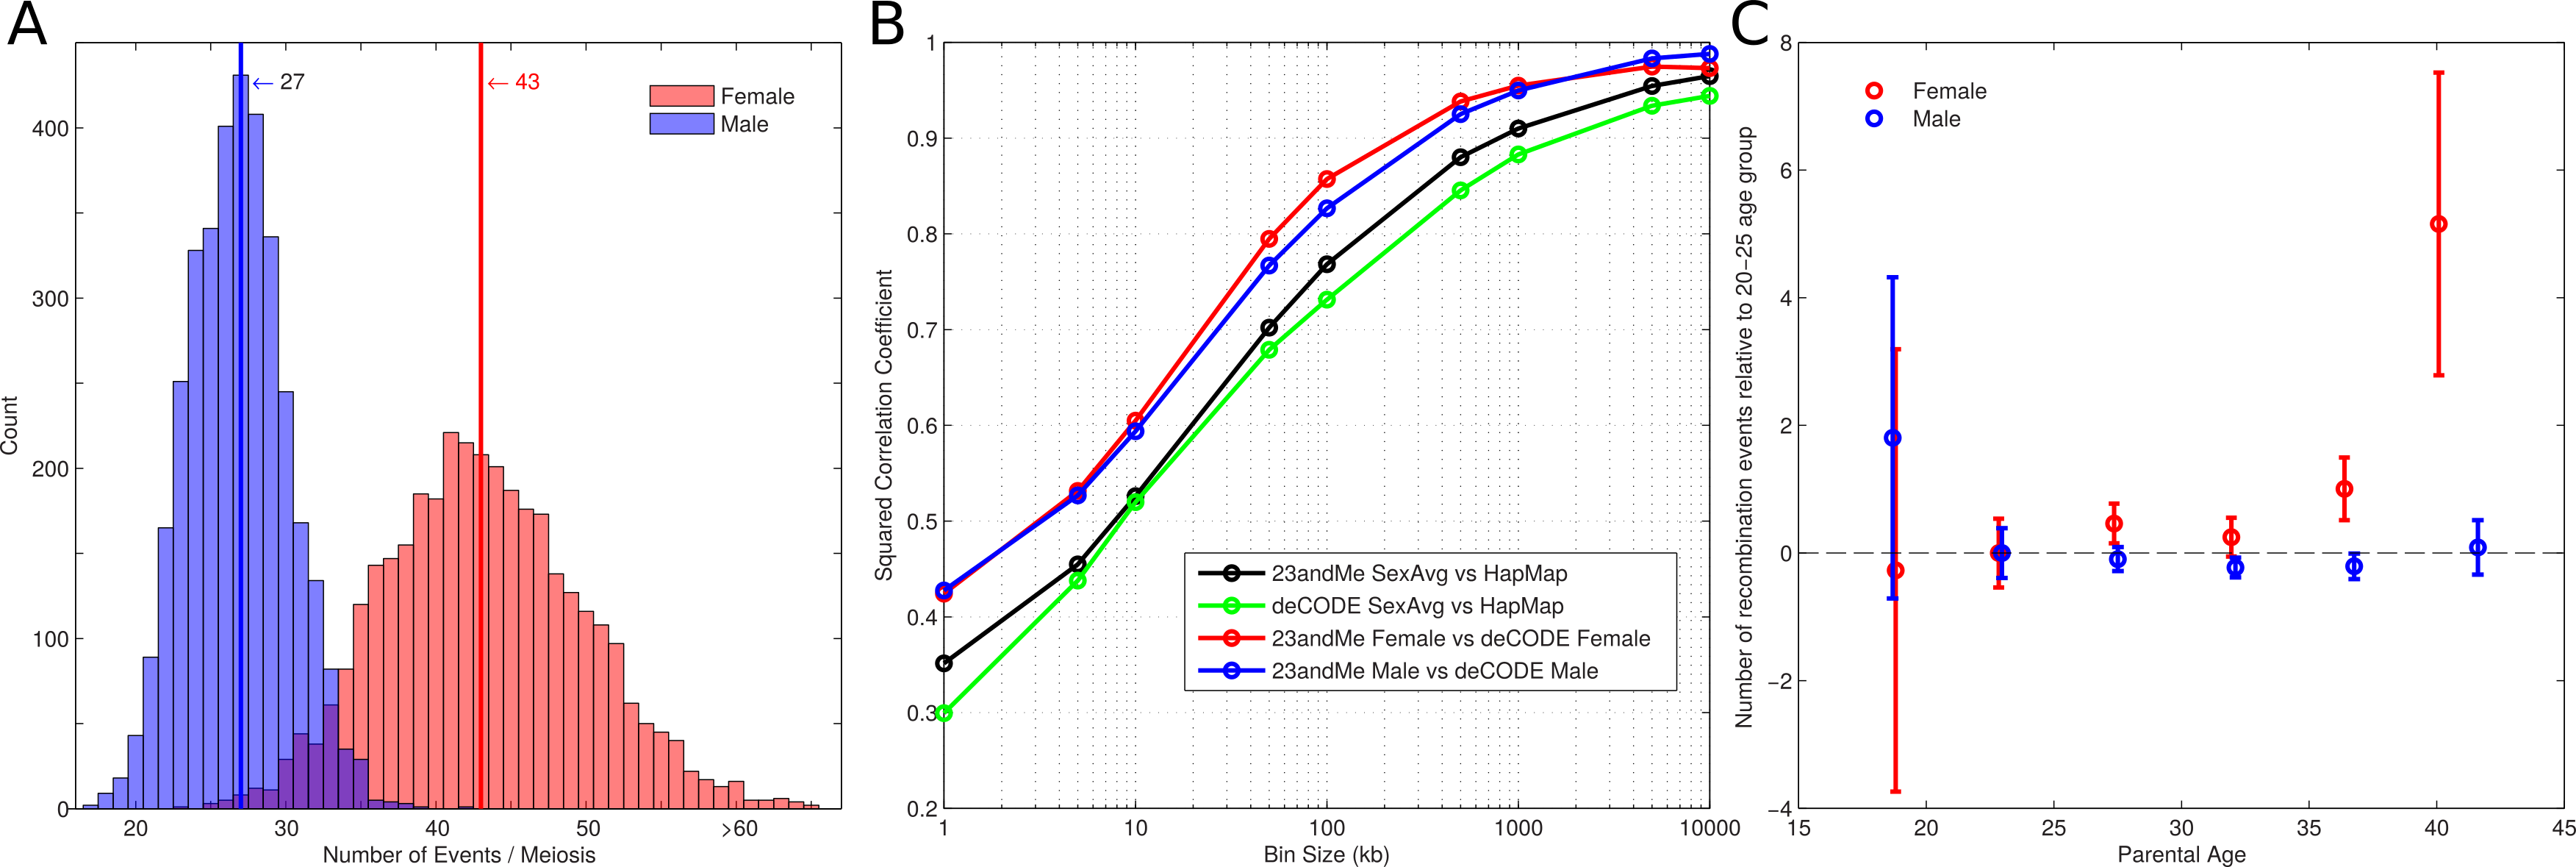
\includegraphics[width=\textwidth]{cointEscape/figs/Figure1.png}
    \vspace{-20pt}
    \captionTitle{\textbf{Properties of recombination partitioned by sex and age.}}{ 
        (a) The number of events per meiosis for females (red, n $=$ 9152) and males (blue, n $=$ 9150), with median values indicated by a vertical line. For phase-unknown individuals, the average number of events per meiosis was used. 
        (b) Squared Pearson correlation between the 23andMe map, the deCODE map and the HapMap map, as a function of scale. 
        (c) The number of recombination events as a function of parental age for females (red, n $=$ 9152) and males (blue, n $=$ 9150), relative to parents of between 20 and 25 years of age. Parents were grouped into 5-year age bins, and the mean number of events estimated. Error bars show a 95\% confidence interval for each group.
    \label{fig:cointF1}}
\end{figure}

Treating the overall recombination rate as a phenotype, we
replicate genetic associations at genome-wide significance for
RNF212, which is known to be essential for crossover-specific
complexes\cite{Reynolds2013}, and within the vicinity of TTC5, which appears
to replicate an association with CCNB1IP1 (\citet{Kong2014}). Another
association near SMEK1 also replicates discoveries elsewhere\cite{Kong2014},
but not at genome-wide significance (Supplementary Table 4).

Previous reports have suggested increased recombination rates
in older females\cite{Kong2004,Coop2008}. Using linear regression (Supplementary
Fig. \ref{fig:cointFS6}), we obtain a similar result with an additional 0.067
events per year being observed in females ($P=$ 0.002, F-test), and
no such effect being observed in males ($P=$ 0.30, F-test). The
female effect appears to be driven by sharp increase in the
number of recombination events for older mothers (Fig. \ref{fig:cointF1}c).
Fitting the piecewise-linear model with a single change point
infers a rapid increase in the female recombination rate after 38.8
years, increasing from 0.047 events per year to 2.990 events per
year. On average, mothers of 39 years and over have an additional
2.51 events compared with younger mothers ($P=$ 0.0005,
Mann-Whitney U).

One possible interpretation of the increasing number of
recombination events with maternal age is that mothers with
higher recombination rates can maintain fertility until a later
age\cite{Kong2004} . To investigate this possibility, we focused on 776 mothers
(providing 2,184 meioses) that were part of larger families and
could have recombination events assigned to specific children.
After subtracting off the average age and average number of
recombination events for each mother, the resulting regression
does not find a significant association with age ($P=$ 0.11, F-test),
although we estimate our power to detect an effect size of an
additional 0.067 events per year in this subsample to be no more
than 30\%.

Both pedigree and LD studies have suggested that $\sim$60-70\% of
crossover events occur within recombination hotspots\cite{Coop2008,Myers2005}. Our
data confirm this result with 62.7\% of events occurring within
LD-defined hotspots in females, and 67.3\% occurring within
hotspots in males (Fig. \ref{fig:cointF2}a; Supplementary Fig. \ref{fig:cointFS7}A). The 4.6\%
difference between the two sexes is highly significant
($P=$ \num{1.1e-69}, Mann-Whitney U), suggesting differences in
the regulation of crossover placement between the sexes. The
result remains significant after thinning the female data to match
the crossover density of the male data ($P<$ \num{2.2e-16},
Mann-Whitney U), and does not appear to be driven by
increased male recombination rates near the telomeres (see
Supplementary Methods).

Hotspot localization is believed to be under the control of the
zinc-finger protein PRDM9, which recognizes and binds specific
DNA motifs\cite{Berg2010,Berg2011,Hinch2011,Parvanov2010}. We find single-nucleotide polymorphisms
(SNPs) in the vicinity of PRDM9 to be strongly associated with
the degree of hotspot usage, as has previously been reported\cite{Kong2014,Hinch2011}.
The most strongly associated SNP is rs73742307 achieving a
P value of \num{7.9e-184} (\citet{Reynolds2013}), with no other region achieving a
genome-wide significant association with this phenotype
(Supplementary Table 5).

Variation within the PRDM9 DNA-binding domain can result
in changes to the recognized motif and hence lead to differences
in hotspot localization between individuals. While the major allele
of PRDM9 (allele A) is present at high frequency in most human
populations, a large number of low-frequency alleles have been
observed, particularly within African populations\cite{Berg2011,Parvanov2010}. Consistent
with this, we find hotspot usage to be significantly lower within
individuals of African ancestry (Fig. \ref{fig:cointF2}b; Supplementary Table \ref{tab:cointTS6}),
which reflects the fact that the LD-defined hotspots are expected
to mostly represent the common PRDM9 allele. Notably, while
over 75\% of our data are derived from individuals of European
ancestry, hotspot usage is higher for males than females across all
ancestries.

\begin{figure}[h]
    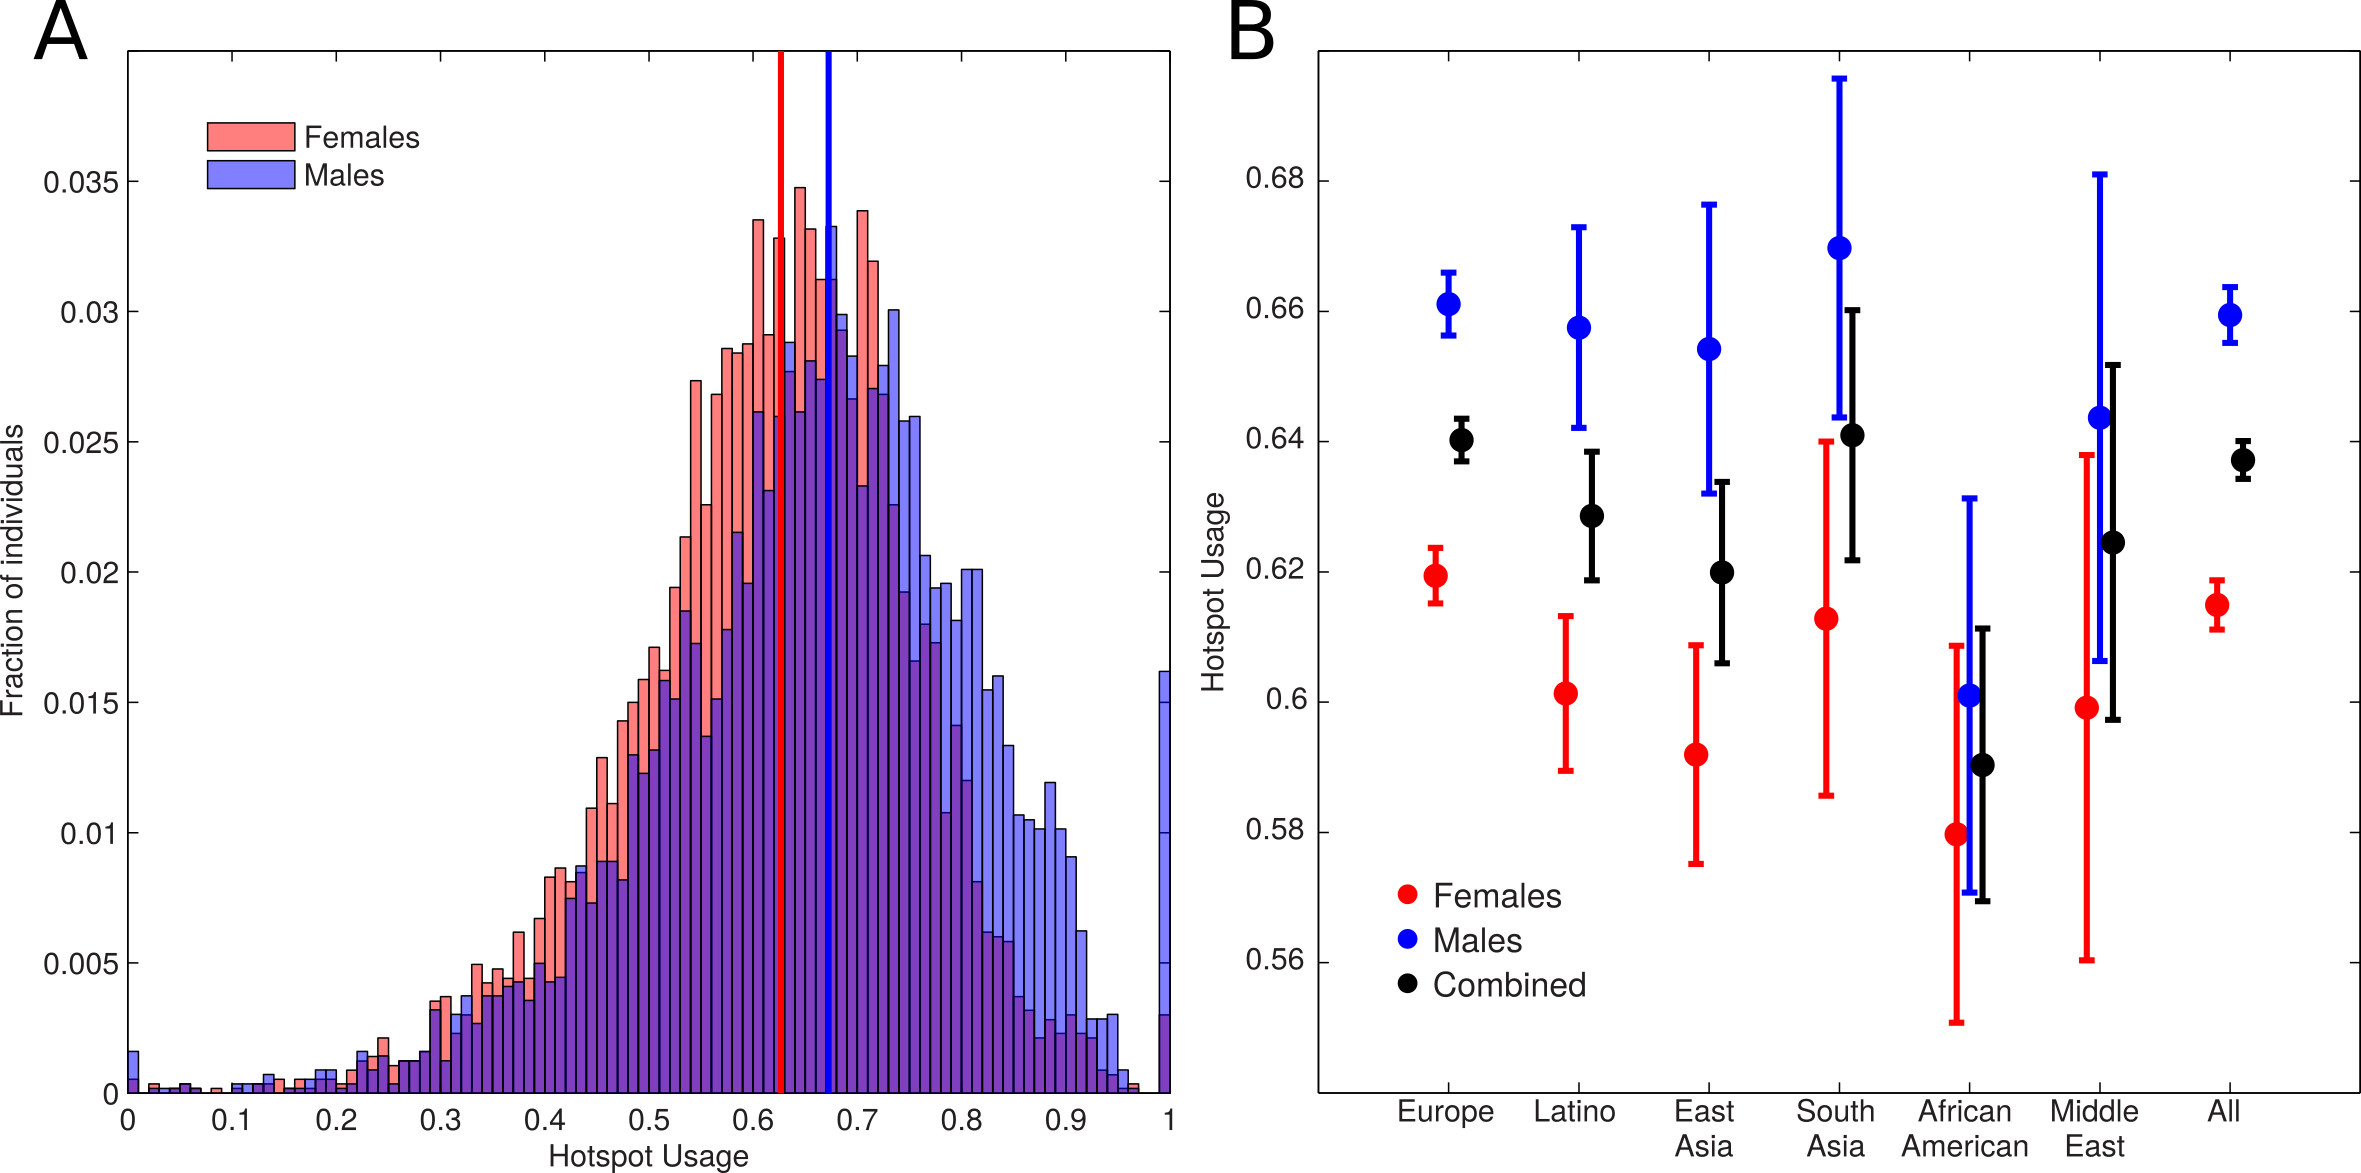
\includegraphics[width=\textwidth]{cointEscape/figs/Figure2.png}
    \vspace{-20pt}
    \captionTitle{\textbf{Sex differences in recombination hotspot usage.}}{
        (a) Hotspot usage for female (red, n $=$ 9152) and male (blue, n $=$ 9150) meioses. Median values for each sex are shown by vertical lines. 
        (b) Mean hotspot usage, subdivided by parental population. Females are shown in red, males in blue and a combined estimate in black. Error bars indicate a 95\% confidence interval.
       \label{fig:cointF2}}
\end{figure}

We find a weak association between hotspot usage and
maternal age (Supplementary Fig. \ref{fig:cointFS7}B). Using logistic regression,
we estimate a decrease in hotspot usage corresponding to
$\sim$1\% over a 10-year period ($\beta_1=$ \num{-0.0042}, $\text{s.e.}=$ \num{9.6e-4}, 
$P=$ \num{1.2e-5}, F-test). To ensure this effect is not driven by
differences in parental ancestry within the sample, we repeated
the analysis only using individuals of European ancestry. In this
case, the effect size remains similar ($\beta_1=$ \num{-0.0033}, $\text{s.e.}=$ 0.0013),
but is only marginally significant ($P=$ 0.0101, F-test). Including
the number of events as an additional predictor variable within
the regression leaves age as a weakly significant predictor
($P=$ 0.0106, F-test), but not the number of events ($P=$ 0.74,
F-test). Despite the small size of the estimated effect, we note that
no such age-related effects were observed in males.

To learn more about interactions between recombination
events, we used the high number of crossover locations in our
data to better characterize the phenomenon of crossover
interference. By considering the distribution inter-crossover
distances, we fit three models to describe the distribution of
inter-crossover distances: a model without interference between
crossovers (also known as the gamma model of crossover
interference\cite{Broman2000}), and a mixture model in which a subset of
events come from a process that exhibits no interference (also
known as the Housworth-Stahl model\cite{Housworth2003}). To fit these models, we
used existing methods for families in which recombination events
could be assigned to specific individuals, and extended these
methods for smaller families where recombination events cannot
be simply assigned to a specific individual (see Supplementary
Methods).

In agreement with previous reports\cite{Housworth2003,Fledel-Alon2009}, the Housworth-Stahl
interference escape model provides a much better fit to our
data than either the gamma simple interference model or the
interference-free model (Fig. \ref{fig:cointF3}a). Under this model, the estimates
of the strength of crossover interference are similar to previous
reported using smaller data sets\cite{Fledel-Alon2009}. The degree of interference is
inferred to be lower in females than in males ($\nu_{female}=$ 7.19 vs
$\nu{male}=$ 8.93). In addition, 7.8\%/6.7\% of female/male events are
inferred to escape interference. We therefore conclude that a
non-negligible fraction of crossovers occur in the absence of
crossover interference.

We find evidence that both the degree of interference and
interference escape varies across chromosomes (Fig. \ref{fig:cointF3}b,c;
Supplementary Table \ref{tab:cointTS7}). The strength of interference is reasonably 
well predicted by the chromosome map length ($r^2=$ 0.565,
$P=$ \num{6.4e-9}), although the relationship is only significant in
females when considering the sexes separately ($r^2_{female}=$ 0.69,
$P=$ \num{1.7e-6} and $r^2_{male}=$ 0.172, $P=$ 0.06; Supplementary Fig. \ref{fig:cointFS8}).
In contrast, the fraction of events escaping interference shows no
relationship with chromosome map length ($r^2=$ 0.001, $P=$ 0.84).
Certain chromosomes appear to have high degrees of escape, with
chromosomes 8, 9 and 16 (in females) being notable outliers.

\begin{figure}[h]
    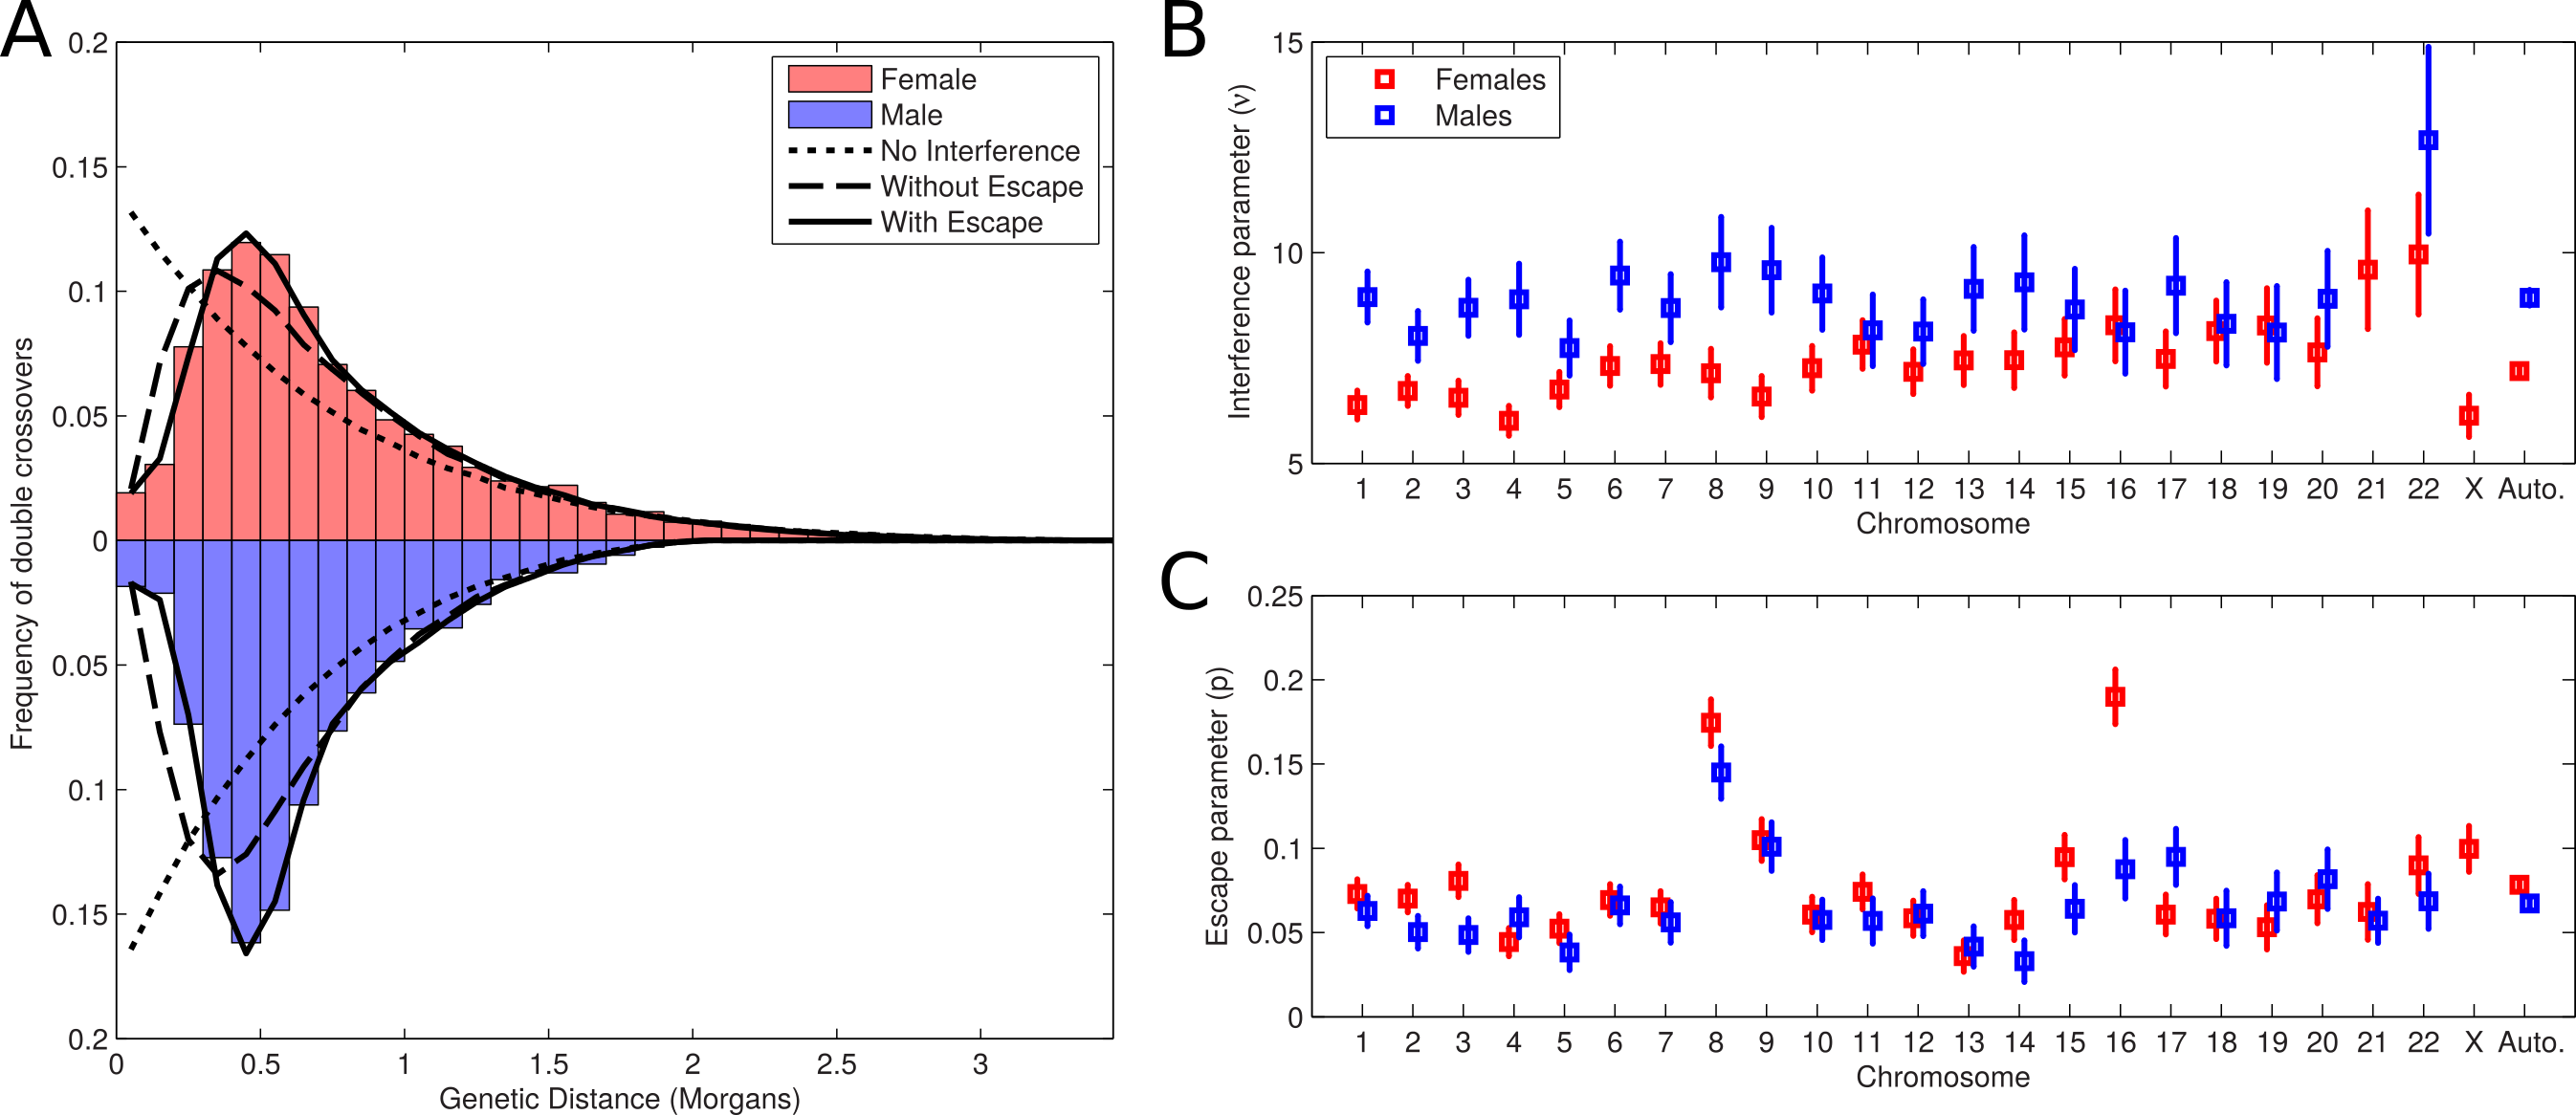
\includegraphics[width=\textwidth]{cointEscape/figs/Figure3.png}
    \vspace{-20pt}
    \captionTitle{\textbf{Estimation of crossover interference parameters.}}{
        (a) Fit of three models of interference to the inter-crossover distances observed on chromosome 1, derived from phase-known mothers (red, n $=$ 2184) and fathers (blue, n $=$ 2092).
        The interference-free model is shown as a dotted line, the gamma simple interference model is shown as a dashed line and the Housworth-Stahl interference escape model is shown as a solid line. 
        (b) Per-chromosome estimates of the interference parameter as estimated from the Housworth-Stahl interference escape model.
        Error bars indicate a 95\% confidence interval.
        Note that chr21 in males is excluded due to an extremely high estimate.
        (c) Per-chromosome estimates of the proportion of events escaping interference. Error bars indicate a 95\% confidence interval.
       \label{fig:cointF3}}
\end{figure}

To investigate whether crossover interference changes with
parental age, we subdivided our data into 10 quantiles on the
basis of age, and fit the Housworth-Stahl interference escape
model to each group independently. We observe a striking
increase in the proportion of events that escape interference with
maternal age (Fig. \ref{fig:cointF4}a), rising from 6.7\% for mothers under 25
years to 9.5\% for mothers over 35 years. No such correlation is
observed for the interference parameter in females, and no
correlation is observed for either parameter in males
(Supplementary Fig. \ref{fig:cointFS9}). The effect is robust to different subdivisions % edited typo
of the data (Supplementary Figs \ref{fig:cointFS10} and \ref{fig:cointFS11}).

A potential concern is that the detected increase in interference
escape could be driven by the observed increased number of
crossovers in older mothers. If the number of crossovers is 
increased, then the distances between them are necessarily
shorter, which may in turn influence the interference parameter
estimates. To account for this possibility, we performed stratified
sampling of individuals to control for the number of events
within each quantile. The observed increase in the escape
parameter with maternal age is still observed (Supplementary
Fig. \ref{fig:cointFS12}), indicating that it is not driven by changes in the overall
recombination rate.

To further investigate the differences between old and young
parents, we plotted the distribution of inter-crossover distances
for young and old parents (Fig. \ref{fig:cointF4}b,c). The interference escape
effect in females appears to be predominately driven by an
increase in the number of very tightly clustered events, generally
separated by less than $\sim$5 cM. These tightly clustered events are
not well captured by the Housworth-Stahl interference escape
model (Supplementary Fig. \ref{fig:cointFS13}), and a major concern therefore is
that these tightly clustered events represent false-positive calls
arising from genotyping error. However, the effect remains even
if we apply much stricter filtering of the crossover events
(Supplementary Fig. \ref{fig:cointFS14}), and in addition we believe genotyping
error is unlikely to explain the association between the escape
parameter and maternal age because (a) the effect is not seen in
males, and (b) it would imply increased genotyping error for
older mothers (but not fathers).

\begin{figure}[h]
    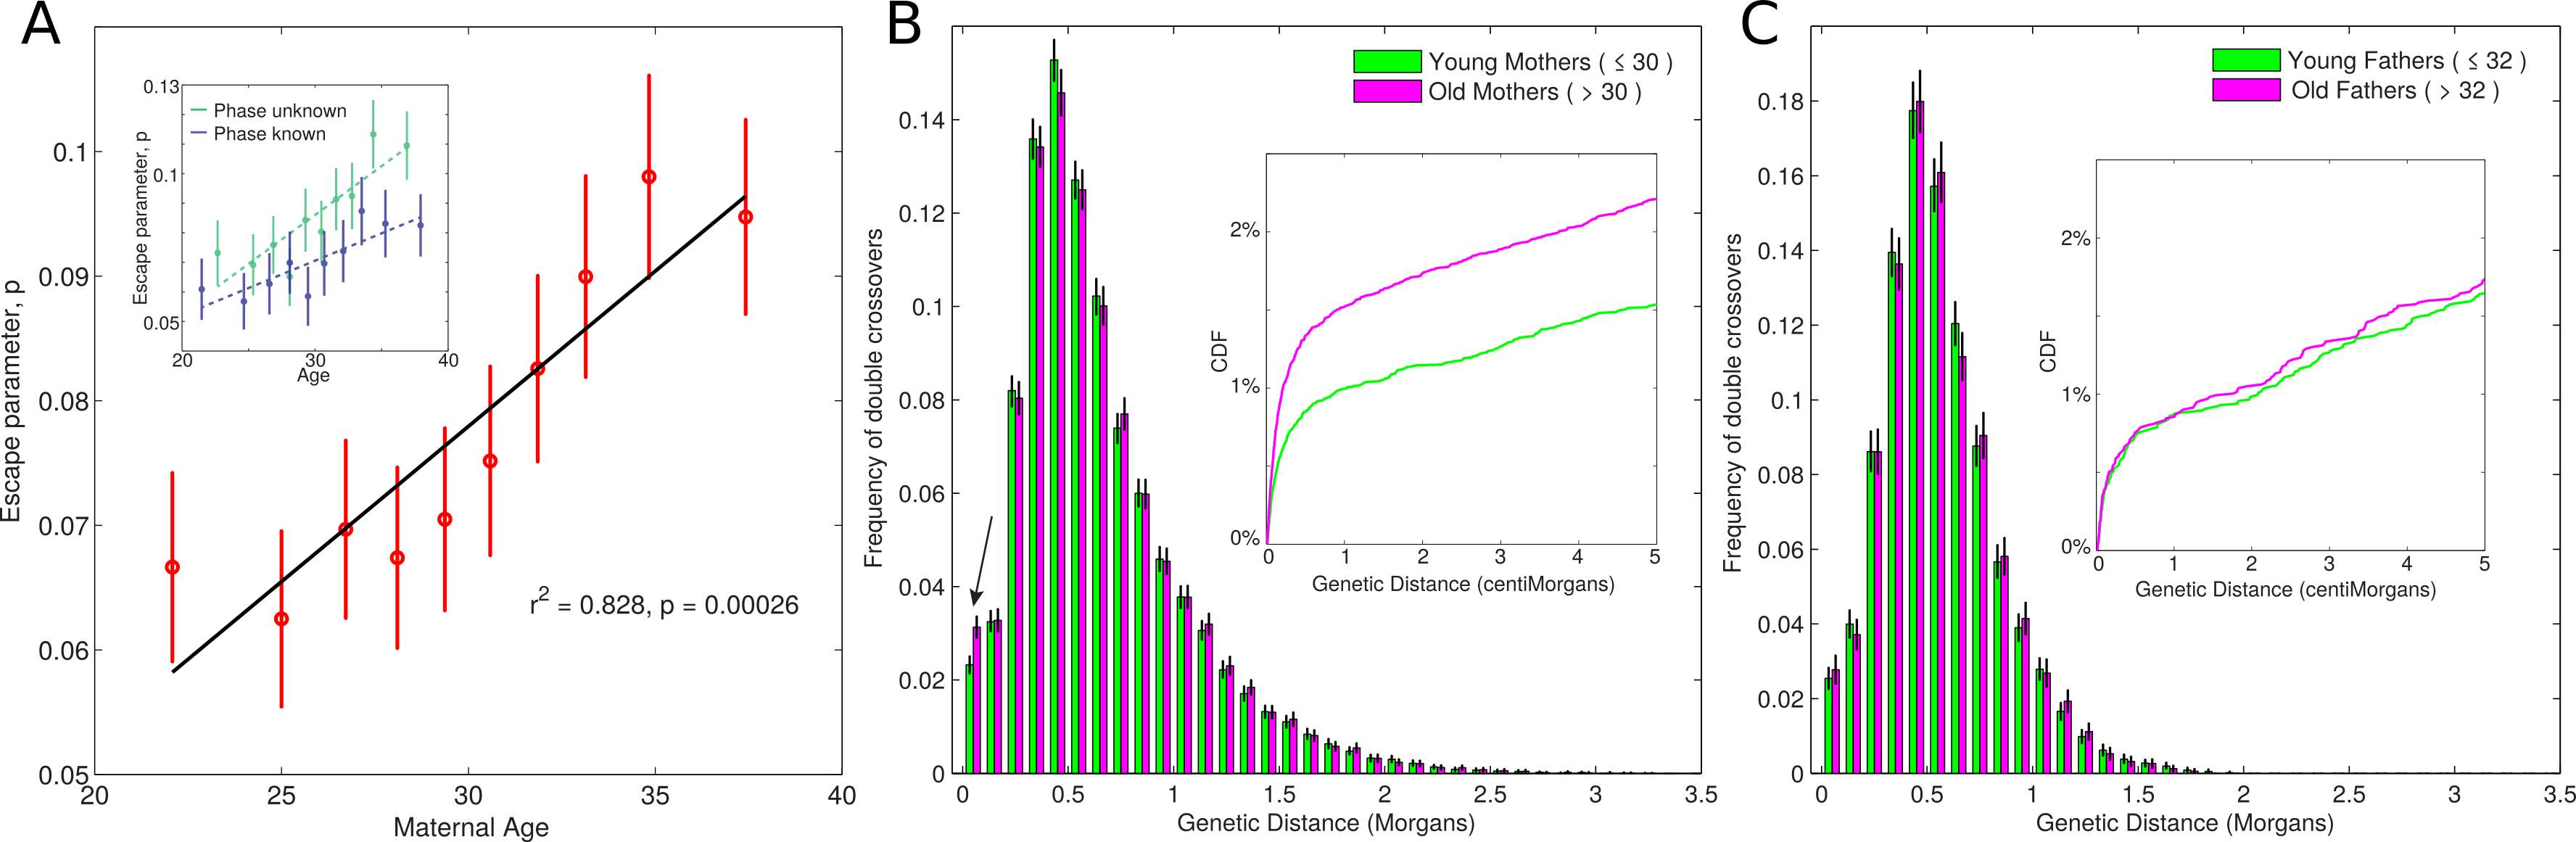
\includegraphics[width=\textwidth]{cointEscape/figs/Figure4.png}
    \vspace{-20pt}
    \captionTitle{\textbf{Departures from simple crossover interference.}}{
        (a) Inferred escape parameter as a function of maternal age.
        Mothers were divided into 10 approximately equal-sized deciles on the basis of age, and the Housworth-Stahl interference escape model was fitted for each group separately.
        The inset shows the estimates of the escape parameter when considering phase-known (blue, n $=$ 2184) and phase-unknown (green, n $=$ 6968) individuals separately. 
        Estimates for $\nu$ show no correlation with age (Supplementary Fig. \ref{fig:cointFS9}). Error bars indicate 95\% confidence intervals. 
        (b) Distribution of inter-crossover distances for young and old mothers, where the boundary between young and old is taken as median maternal age (30 years). 
        Error bars represent a 95\% confidence interval assessed via 1000 bootstrap samples, and the arrow highlights a significant difference between the young and old groups for tightly clustered events. 
        The inset shows the cumulative distribution function (CDF) up to 5 cM. 
        (c) Distribution of inter-crossover distances for young and old fathers, where the boundary between young and old is taken as median paternal age (32 years).
       \label{fig:cointF4}}
\end{figure}

In terms of meiosis, a major difference between the sexes is that
female meiosis starts during fetal development, but does not
complete until adulthood. As such, while male gametes are
produced throughout adulthood and promptly proceed through
meiosis, oocytes remain arrested in a late stage of prophase
(dictyotene) for many years, if not decades. Presuming our
observation of increasing crossover interference escape with
maternal age is not due to some obscure form of genotyping
error, our observations add to similar evidence of increasing rates
of recombination\cite{Kong2004} and aneuploidy\cite{Hassold2001} in aging females. Although
these phenomena are presumably related, the biological
mechanisms by which they occur are unclear, and we can think
of at least three possibilities. First, given chromatids remain
physically proximal during the extended period of female meiotic
arrest, one possible explanation is that additional recombinations
are initiated during this time, perhaps in response to
DNA damage. However, as recombination is believed to have
completed by the time of dictyotene, such an explanation appears
unlikely. A second possibility, previously invoked to explain the
increasing recombination rate with maternal age\cite{Kong2004}, suggests
oocytes with additional recombination events could be at
reduced risk of nondisjunction, and hence would be more likely
to lead to viable embryos in older mothers. However, it is not
clear that this mechanism would explain the increased clustering
of events observed in our data. Finally, a third possibility is 
related to the so-called ``production line'' hypothesis, in which
oocytes are selected for maturation sequentially in the same order
as their generation, and later oocytes have therefore potentially
undergone additional mitotic divisions prior to entering
meiosis\cite{Reizel2012}. However, the existence of a production line has been
debated for many years\cite{Reizel2012,Polani1991,Rowsey2014}, and so the likelihood of this
explanation is unclear.

%%%%%%%%%%%%%%%%%%%%%%%%%%%%%%%%%%%%%%%%
%%%%%%%%%%%%%%%%%%%%%%%%%%%%%%%%%%%%%%%%
\section{Methods}
%%%%%%%%%%%%%%%%%%%%%%%%%%%%%%%%%%%%%%%%
%%%%%%%%%%%%%%%%%%%%%%%%%%%%%%%%%%%%%%%%

\paragraph{Sample genotyping.} Samples were collected and genotyped at the consumer
genetics company 23andMe Inc., as described previously\cite{Eriksson2010}. Briefly, genotyping was
performed on genomic DNA extracted from saliva samples. DNA was genotyped
on one of two microarray platforms: the Illumina HumanHap550+ BeadChip
platform, which includes more than 550,000 SNPs, or the Illumina
HumanOmniExpress+ BeadChip, which has a base set of 730,000 SNPs
augmented with $\sim$250,000 SNPs to obtain a superset of the HumanHap550+,
as well as a custom set of about 30,000 SNPs.

\paragraph{Pedigree construction.} Pedigrees were constructed first by identifying trios using
estimated identity-by-decent relationships. Trios were then combined to form
nuclear families, and nuclear families were joined based on the assumed
relationships to form larger pedigrees. We identified trios by finding triplets of
individuals in the 23andMe customer cohort that had estimated identity-by-decent
relationships matching those expected in a true trio. Trios were accepted if both
parents were at least 18 years old upon the birth of the child and one parent was
male and the other female. We created nuclear families by identifying all trios with
the same two parents and then by combining the children of these trios. Finally,
larger pedigrees were created by simply joining the nuclear families based on the
assumed relationships and by accounting for directionality given by the age of
individuals. Any two individuals with more than one potential relationship were
excluded along with the pedigrees they belonged to.

\paragraph{Calling of recombination events and data filtering.} Prior to data filtering,
the data set consisted of 4,270 pedigree families, with data pertaining to 18,647
informative meioses. This raw data set consisted of 692,876 recombination events,
with a median of 45 and 28 events per meiosis in females and males, respectively.

The Merlin algorithm (version 1.1.2) used to detect recombination events does
not account for genotyping error, and genotyping errors are therefore likely to
result in spurious recombination event calls. To account for this issue, our first step
was to only use high-confidence sites. First, we required the sites to have a call rate
greater than 90\% and Hardy-Weinberg $P$ value $\le$ \num{1e-20} (as calculated in the
23andMe cohort). Second, we excluded sites with minor allele frequencies differing
from those of the 1000 Genomes Phase 1 reference panel\cite{1000G2012}. This was achieved by
constructing a 2 $\times$ 2 contingency table and comparing the 1000 Genomes
European allele counts with those from 2,000 randomly selection 23andMe
customers, and using a $\chi^2$-test to identify significant deviations. Sites with $P$ values
less than \num{1e-15} were removed.

Having applied these basic site filters, we next aimed to remove any weakly
supported recombination events. This was achieved by first using the Merlin ``error''
feature to remove potential genotyping errors not consistent with gene flow within
each pedigree. In addition, we excluded all recombination events supported by less
than three recombination-informative sites on either side, where we define an
informative site as a site that is called as heterozygotic in exactly two individuals
out of each mother-father-child trio. Finally, we removed all pairs of events within
each single family that occurred within the same SNP interval. Together, these
filters removed 31,742 weakly supported events, which corresponded to 4.6\% of the
total number.

Preliminary inspection of the genetic maps identified a region on chromosome
10 where the 23andMe genetic map diverged substantially from that generated by
deCODE\cite{Kong2010}. This can be seen in a plot of the chromosome 10 genetic map at
$\sim$50 Mb (Supplementary Fig. \ref{fig:cointFS2}A).

Further investigation of this region revealed a large number of ``double''
crossovers in close proximity to each other (that is, pairs of recombination events
occurring in close proximity within the same individual). While some such
observations are expected through the action of gene conversion, such strong
clustering of these events is not expected biologically. Instead, we believe the result
is suggestive of misplacement of polymorphisms, mis-assembly of one or more
reference contigs in the hg19 reference genome or of more complex types of
error related to copy number polymorphism or array design. In any case, these
double-recombination events represent a form of error that needed to be
eliminated.

To better quantify this issue, we identified all pairs of recombination events
occurring within a single individual that were within 1 Mb of each other. For each
SNP in the genome, we estimated the number of these event pairs that span the
SNP (Supplementary Fig. \ref{fig:cointFS2}B).

For the vast majority of the genome, there were very few such event pairs, and
hence localized peaks likely represent data quality issues. We therefore identified all
SNPs spanned by at least 14 event pairs (with this threshold being equivalent 
to the 99.9th percentile of the distribution). In this way, we identified 50 regions
with strong enrichment of nearby event pairs (Supplementary Table 8). Note that
for this analysis we ignored the pseudoautosome, as a large number of events
occurring in close proximity might be expected due to the extreme male
recombination rate within this region.

The regions with high numbers of clustered events were themselves clustered
into 13 regions across 8 chromosomes, and are often in the vicinity of chromosome
centromeres, telomeres or reference assembly gaps. We removed all event pairs
within 500 kb of the region boundaries described in Supplementary Table 8, which
resulted in the removal of 2,916 events (0.42\% of the total). The removal of these
events improved the concordance between the 23andMe and deCODE maps
(Supplementary Fig. \ref{fig:cointFS2}C).

Previous research using well-curated data in 728 meioses reported an average of
39.6 autosomal events per gamete in females (95\% CI 38.5-40.6), and 26.2
autosomal events per gamete in males (95\% CI 25.6-26.7)7. The minimum/
maximum number of observed autosomal events in any given meiosis in this
data was 19/71 for females, and 16/43 for males (Graham Coop, personal
communication).

Preliminary analysis of our data revealed a small subset of individuals had
biologically unrealistic numbers of recombination events. Our first filtering step
was to remove the pedigrees containing these individuals. Specifically, we removed
individuals (and their containing pedigrees) that were more than 5 s.d. from the
(sex specific) median number of recombination events. To guard against outliers,
we used a robust estimate of the s.d. taken as $\sigma=$ 1.4826 MAD, where MAD
represents the median absolute deviation.

Before filtering, the median number of recombination events was 43 and 27 for
females and males, respectively (including chrX and the pseudoautosome). Using
the $\pm$5$\sigma$ thresholds, we removed pedigrees containing any female with fewer than
10 or more than 76 events per meiosis, or any male with fewer than 9 or more than
45 events. These filters removed a total of 52 pedigrees.

\paragraph{Summary of the filtered data set.} After applying the filtering steps described
above, the filtered data set consists of 4,209 pedigrees containing 18,302
informative meioses, of which 9,152 are from females and 9,150 are from males.
Of the families included in the study, 78.6\% are family quartets, 14.3\% are larger
one-generation families, and 7.1\% are two-generation families (Supplementary
Table 1).

Due to the structure of the pedigrees included in the study, certain
recombination events can be identified as having occurred within a specific child,
whereas others cannot. For example, in family quartets, it is generally unclear
which child has the recombinant haplotype, and we therefore refer to these events
as ``phase unknown''. Conversely, the child containing the recombinant haplotype
can generally be identified in larger pedigree families in which the parental
haplotype can be confidently phased, and we therefore refer to these events as
``phase known''.

In total, 4,276 meioses are derived from phase-known individuals, whereas
14,026 are derived from phase-unknown individuals. Of the female meioses, 2,184
are derived from phase-known mothers and 6,968 are from phase-unknown
mothers. Of the male meioses, 2,092 are derived from phase-known fathers, and
7,058 are derived from phase-unknown fathers.

Individuals were assigned to high-level population groups via comparison with
a set of reference populations (see Supplementary Methods). The majority of
individuals in the data set are of European descent, with $\sim$78\% of the meioses in
the sample occurring within a European individual (Supplementary Table 2).

The parental age distribution for the filtered data set is shown in Supplementary
Fig. \ref{fig:cointFS1}. The mean age was 30 years for females, and 32 for males.

The final filtered data set consists of 645,853 recombination events. Including
the sex chromosomes, the mean number of recombination events was 43.47 for
females ($\sigma=$ 6.64, 95\% CI 43.25-43.69), and 27.04 for males ($\sigma=$ 3.28, 95\% CI
26.94-27.16). For the autosomes alone, the mean number of recombination events
was 41.64 for females ($\sigma=$ 6.34, 95\% CI 41.43-41.85) and 26.61 for males
($\sigma=$ 3.26, 95\% CI 26.51-26.73).

The distribution of interval sizes to which crossovers could be resolved (that is,
the distance between informative markers on either side of the recombination
event) is given in Supplementary Fig. \ref{fig:cointFS3}. Crossovers could be resolved within a
median distance of 28.2 kb.

%%%%%%%%%%%%%%%%%%%%%%%%%%%%%%%%%%%%%%%%
\section{Acknowledgements}
%%%%%%%%%%%%%%%%%%%%%%%%%%%%%%%%%%%%%%%%
We would like to thank Hilary Martin and Julie Hussin for their constructive comments
regarding earlier versions of this manuscript. C.L.C. was supported by the Training
Program in Cellular and Molecular Biology and Genetics, T32 GM007491. Work by
N.A.F., N.E. and D.H. was supported by NIH award 2R44HG006981-02.

%%%%%%%%%%%%%%%%%%%%%%%%%%%%%%%%%%%%%%%%
\section{Author contributions}
%%%%%%%%%%%%%%%%%%%%%%%%%%%%%%%%%%%%%%%%
A.A., D.H. and N.E. designed the study. A.A., C.L.C. and N.A.F. conducted analysis.
A.A. and C.L.C. wrote the paper.

%%%%%%%%%%%%%%%%%%%%%%%%%%%%%%%%%%%%%%%%
\section{Additional information}
%%%%%%%%%%%%%%%%%%%%%%%%%%%%%%%%%%%%%%%%

\paragraph{Supplementary Information} accompanies this paper at \\ \url{http://www.nature.com/naturecommunications}

\paragraph{Competing Financial Interests:} N.A.F. and D.H. are current employees, and N.E. is a
former employee of 23andMe Inc., and have private equity interest. The remaining
authors declare no competing financial interests.

\paragraph{Reprints and permission} information is available online at \\
\url{http://npg.nature.com/reprintsandpermissions/}

\paragraph{How to cite this article:} Campbell, C. L. \textit{et al}. Escape from crossover interference
increases with maternal age. \textit{Nat. Commun.} 6:6260 doi: 10.1038/ncomms7260 (2015).

\bigskip \noindent
This work is licensed under a 
Creative Commons Attribution-NonCommercial-ShareAlike 4.0 International License. The images or
other third party material in this article are included in the article's Creative Commons
license, unless indicated otherwise in the credit line; if the material is not included under
the Creative Commons license, users will need to obtain permission from the license
holder to reproduce the material. To view a copy of this license, visit \\
\url{http://creativecommons.org/licenses/by-nc-sa/4.0/}

%%%%%%%%%%%%%%%%%%%%%%%%%%%%%%%%%%%%%%%%
%%%%%%%%%%%%%%%%%%%%%%%%%%%%%%%%%%%%%%%%
\bibliographystyle{ccampbell_thesis} %unsrtnat} %abbrvnat_noURL} %abbrvUnsrt_last-first} %plain,unsrt,alpha,abbrv,acm,apalike,unsrt
\bibliography{cointEscape/thesis-cointEscape}
%%%%%%%%%%%%%%%%%%%%%%%%%%%%%%%%%%%%%%%%
%%%%%%%%%%%%%%%%%%%%%%%%%%%%%%%%%%%%%%%%

%%%%%%%%%%%%%%%%%%%%%%%%%%%%%%%%%%%%%%%%
%%%%%%%%%%%%%%%%%%%%%%%%%%%%%%%%%%%%%%%%
\beginsupplement
\section{Supplementary Material}
%%%%%%%%%%%%%%%%%%%%%%%%%%%%%%%%%%%%%%%%
%%%%%%%%%%%%%%%%%%%%%%%%%%%%%%%%%%%%%%%%

\subsection{Supplementary Figures}

\begin{figure}[!h]
    %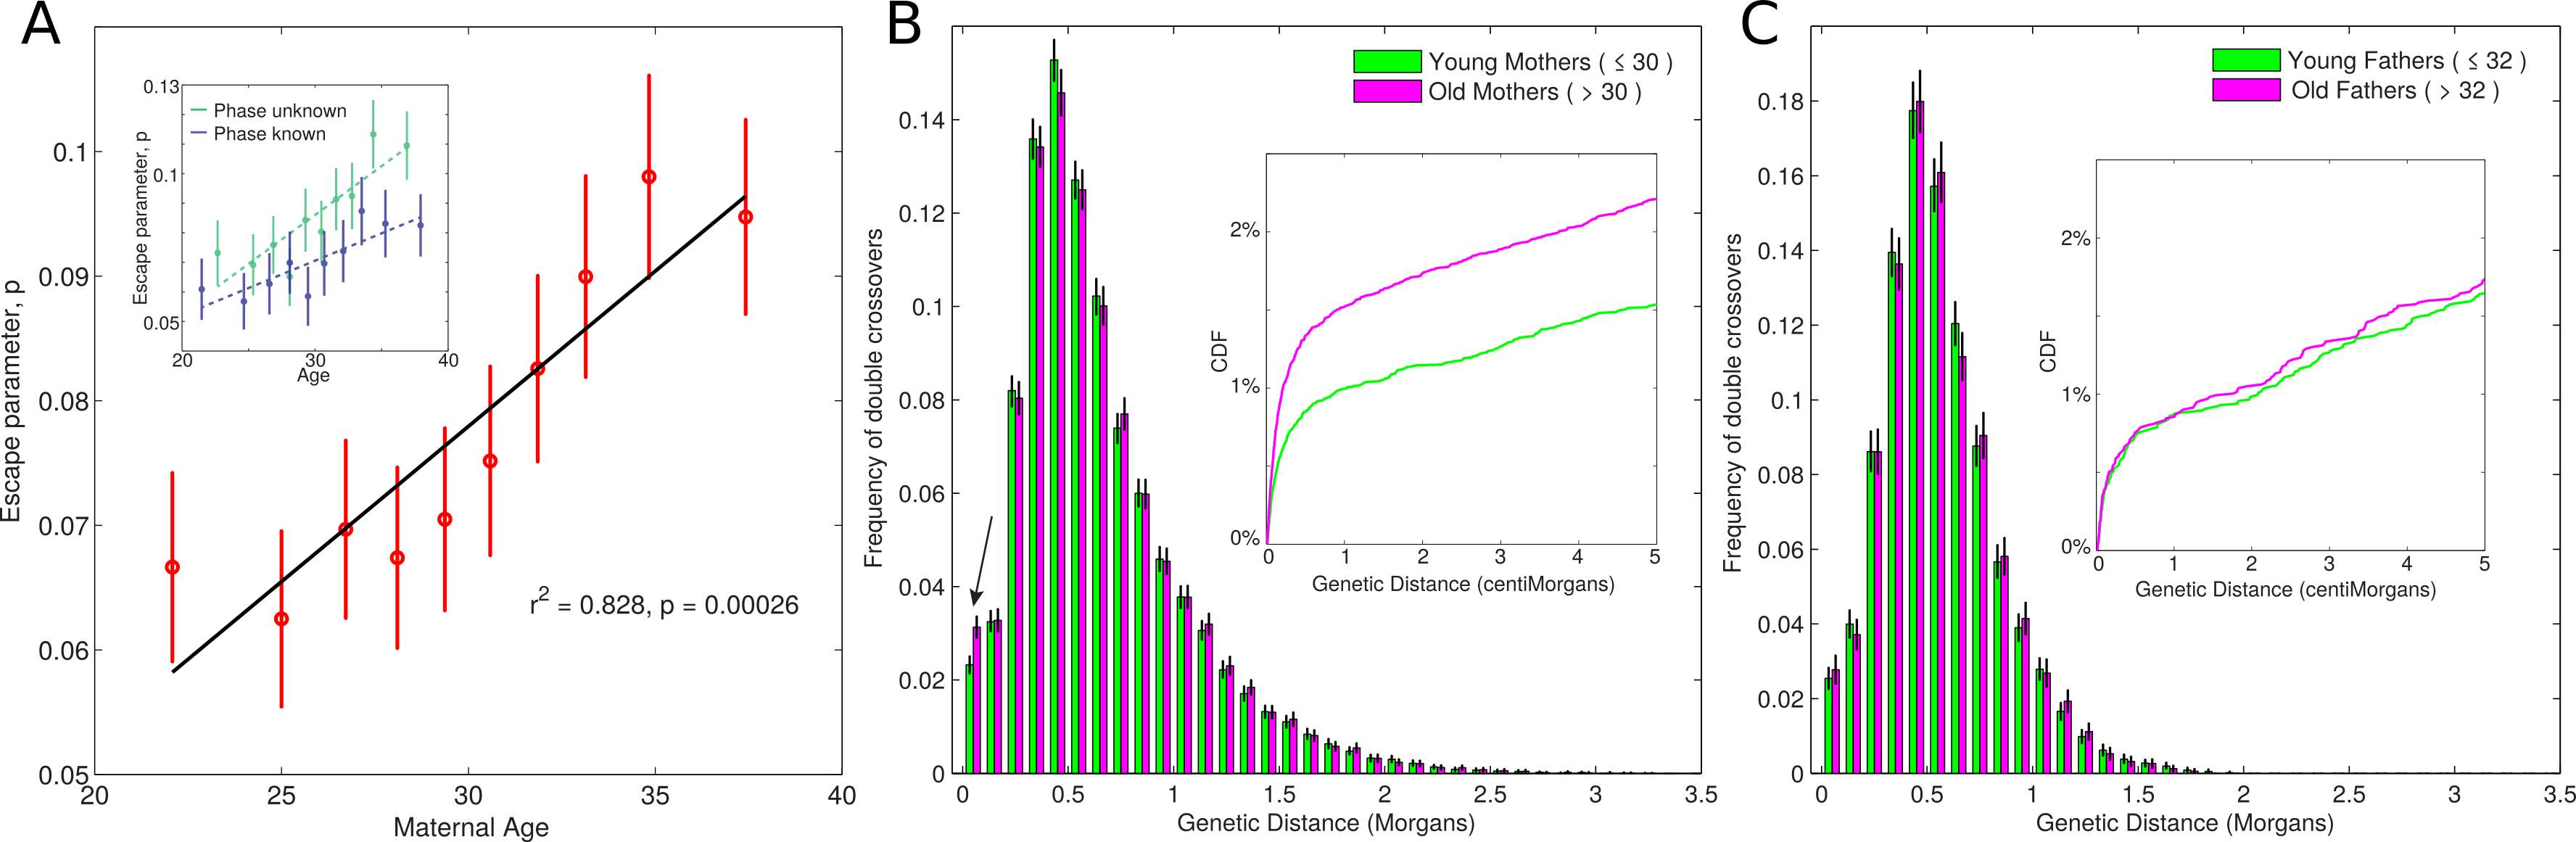
\includegraphics[width=\textwidth]{cointEscape/figs/Figure4.png}
    %\vspace{-20pt}
    \captionTitle{\textbf{Age distributions within the filtered dataset.}}{
        The left hand panel shows the distribution for phase-unknown individuals, where the parental ages were averaged across children. 
        The right hand panel shows data for the phase-known meioses where the parental age at the time of childbirth is known.
        Lines indicate the mean of each distribution. 
        Note that some families were excluded from analysis by 23andMe on the basis age to protect privacy, as seen from the truncated distribution of maternal ages in the right hand panel.  
       \label{fig:cointFS1}}
\end{figure}

\begin{figure}[!h]
    %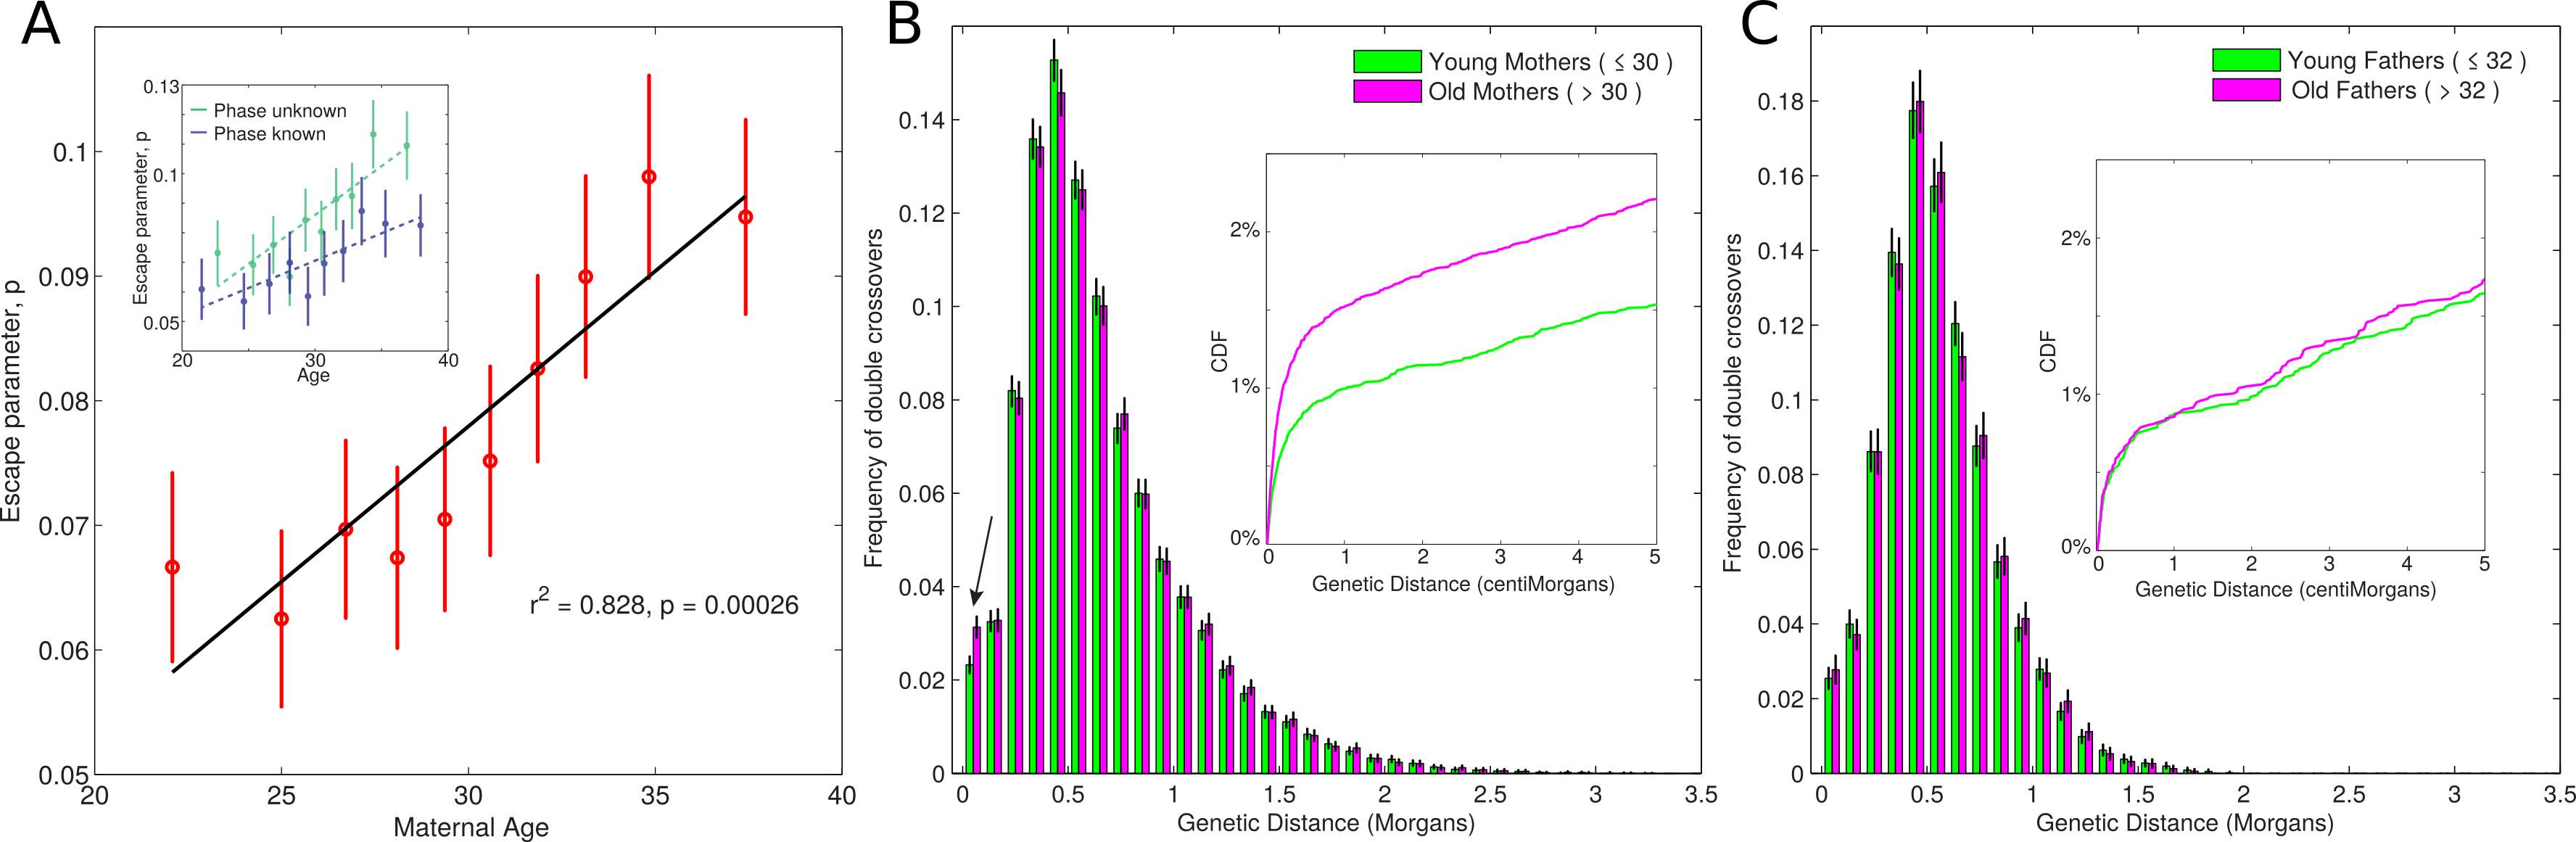
\includegraphics[width=\textwidth]{cointEscape/figs/Figure4.png}
    %\vspace{-20pt}
    \captionTitle{\textbf{Data grooming.}}{
        A) Chromosome 10 map before filtering.
        Genetic maps from the 23andMe data are shown in bold lines, whereas the genetic maps from deCODE are shown as thin lines.
        Separate maps are shown for females(red), males (blue), and sex-averaged (black). 
        Also shown are regions highlighted in grey that represent gaps in the reference assembly, the largest of which being the centromere at around 40Mb.
        B) Clustering of recombination events occurring within 1 Mb of each other within single individuals.
        Each plot shows the number of events within 1 Mb of each other on a log$_{10}$ scale as a function of physical position on each chromosome.
        A large number of these event pairs can be observed on chromosome 10, although other large peaks can also be observed on, for example, chromosomes 8 and 15.
        The dashed line represents the 99.9\% percentile of the distribution, and was used as a threshold for filtering.
        C) Chromosome 10 map after filtering.   
       \label{fig:cointFS2}}
\end{figure}

\begin{figure}[!h]
    %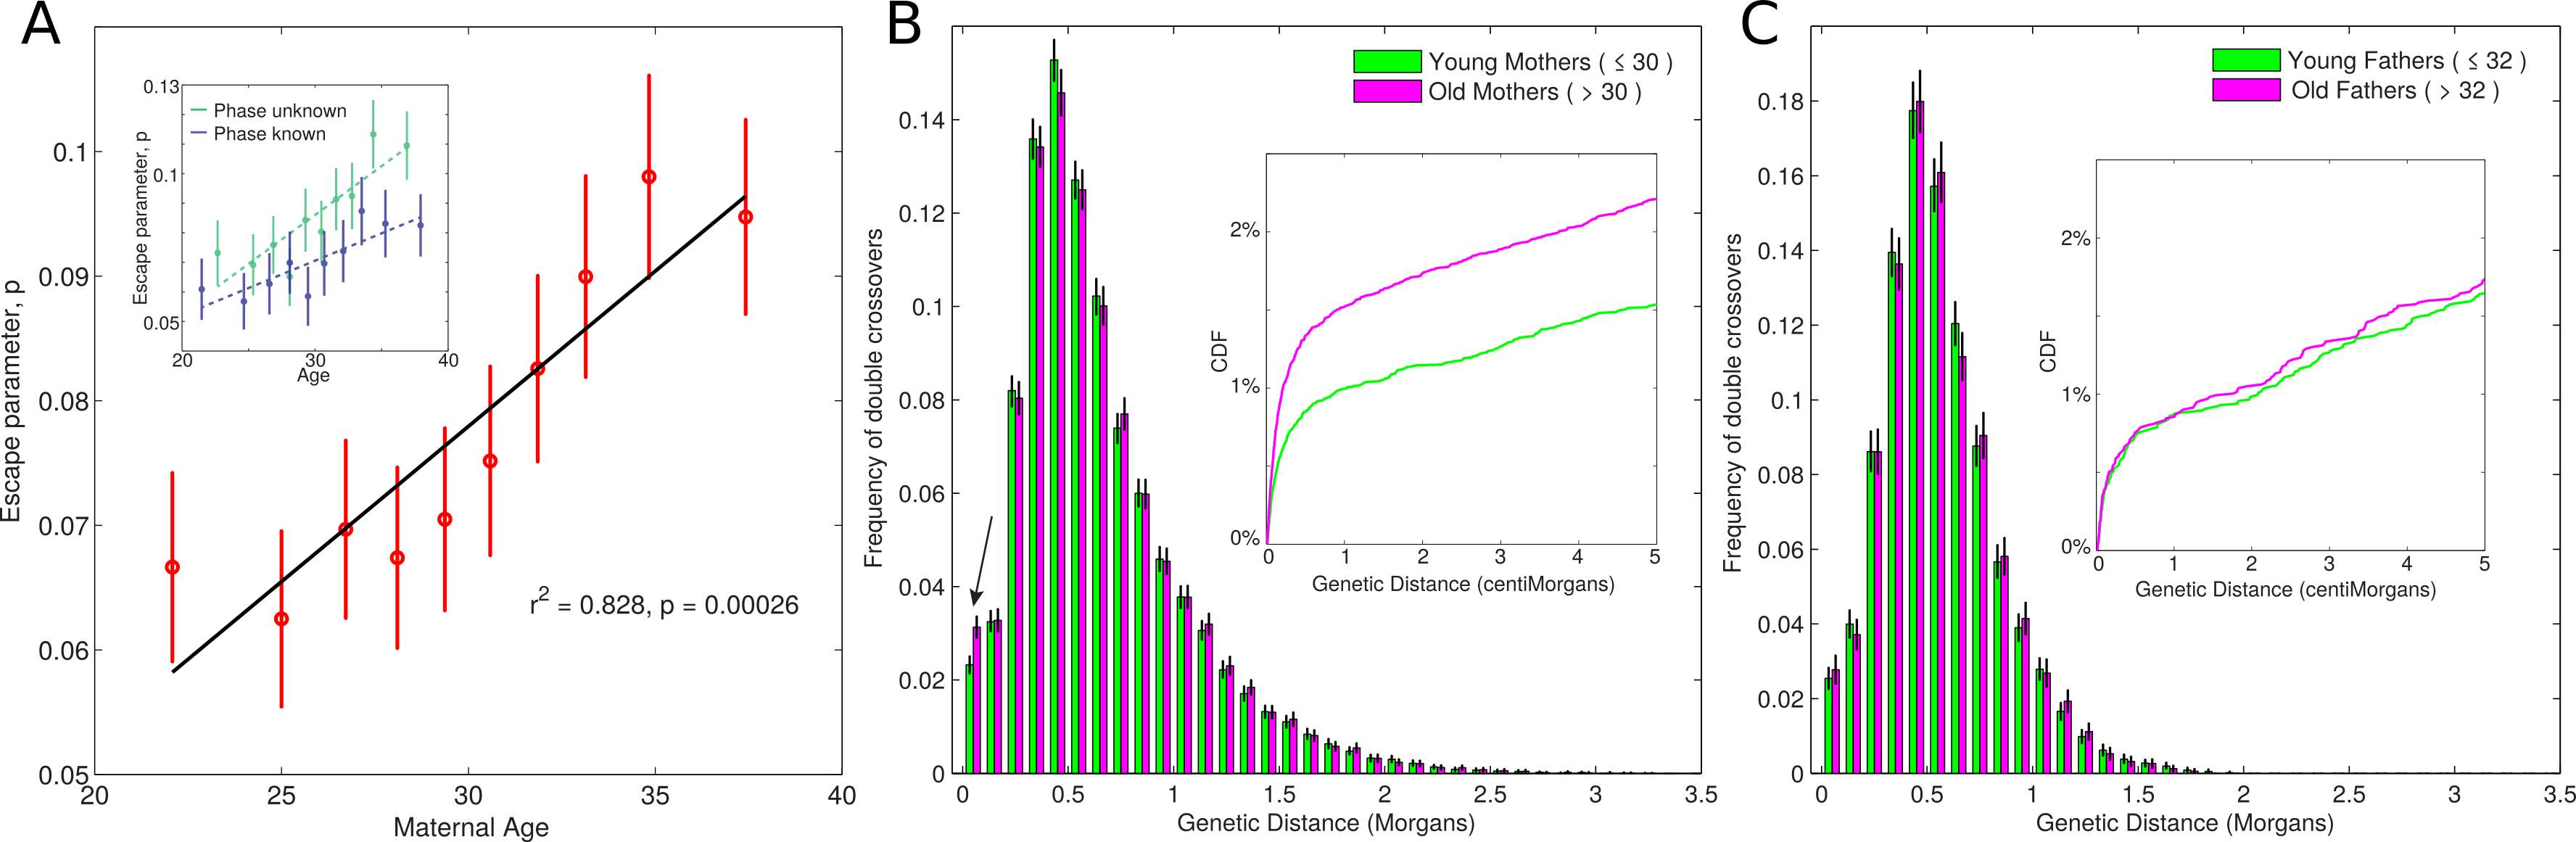
\includegraphics[width=\textwidth]{cointEscape/figs/Figure4.png}
    %\vspace{-20pt}
    \captionTitle{\textbf{Empirical cumulative distance function of crossover localization distances.}} { 
        Red labels indicate the interval distances at the distribution deciles.  
       \label{fig:cointFS3}}
\end{figure}

\begin{figure}[!h]
    %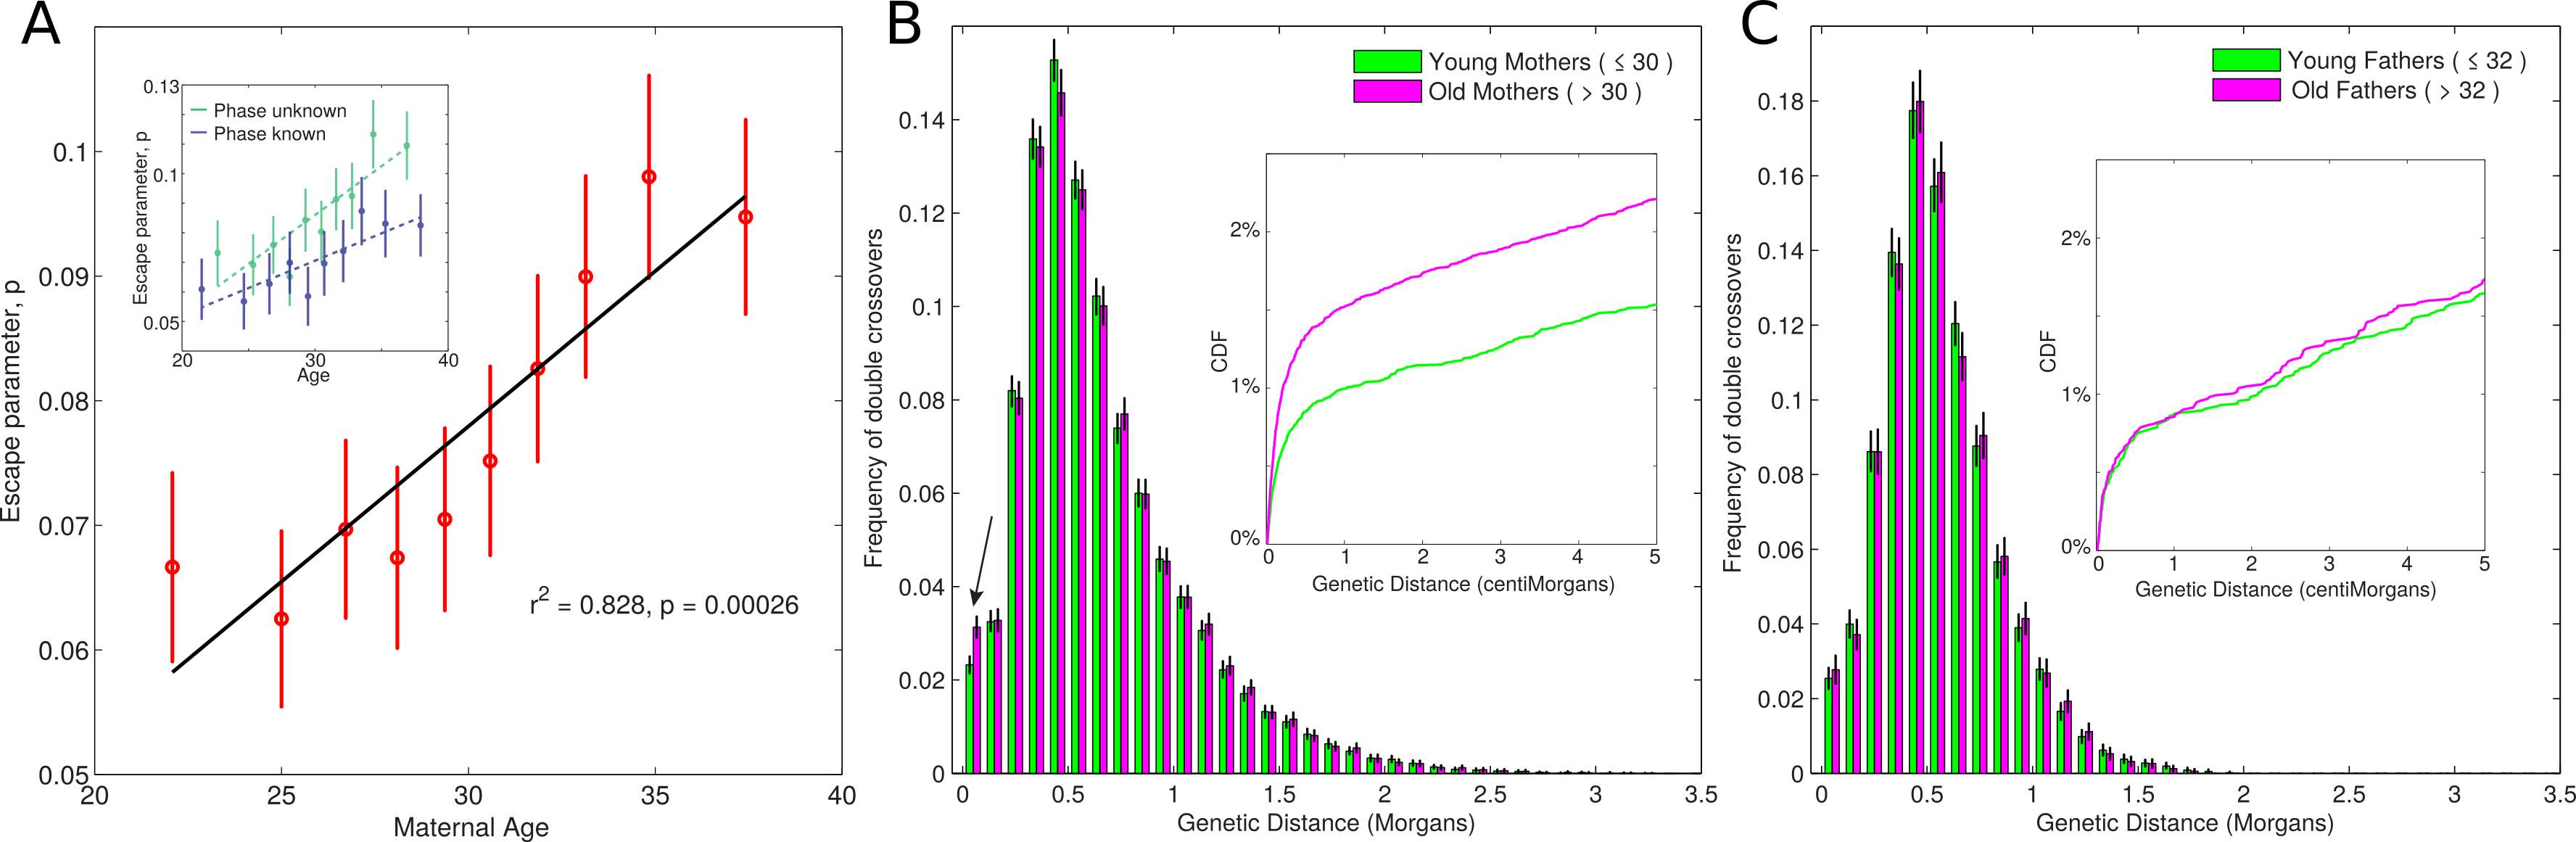
\includegraphics[width=\textwidth]{cointEscape/figs/Figure4.png}
    %\vspace{-20pt}
    \captionTitle{\textbf{Genetic map estimated from 23andMe data.}}{
        Genetic maps from the 23andMe data are shown in bold lines, whereas the genetic maps from deCODE are shown as thin lines.
        Separate maps are shown for females (red), males(blue), and sex-averaged (black).
        Also shown are regions highlighted in grey that represent gaps in the reference assembly. 
        For PAR1, we are showing data derived from Duffy\cite{Duffy2006} for comparison.
        As the deCODE maps cover a slightly smaller physical region than the 23andMe maps, the deCODE maps have been shifted slightly upwards to aid visual comparison.
        Specifically, the deCODE map has been aligned with the 23andMe map at the first physical position within the deCODE map.
        The locations of the alignments are indicated by small circles that can be most clearly seen on the smaller chromosomes.  
       \label{fig:cointFS4}}
\end{figure}

\begin{figure}[!h]
    %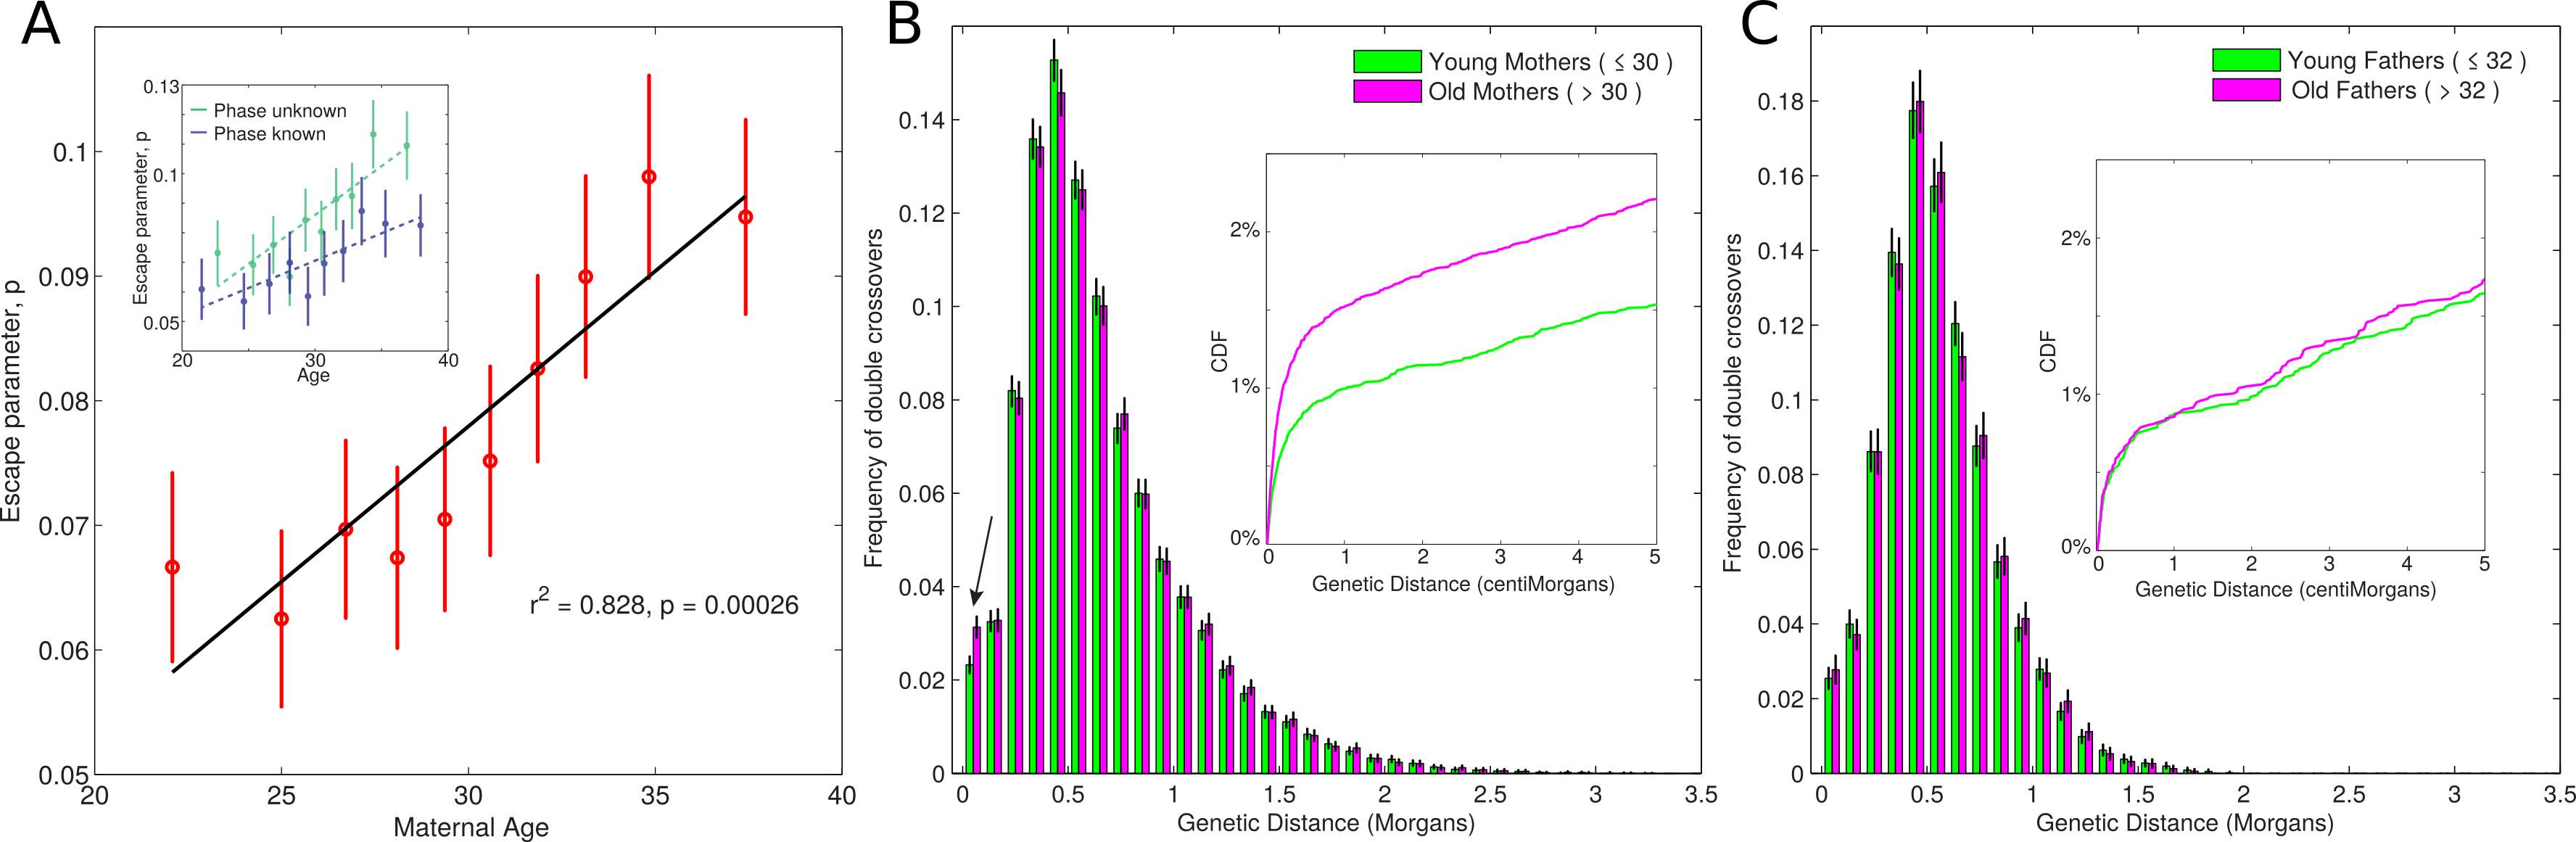
\includegraphics[width=\textwidth]{cointEscape/figs/Figure4.png}
    %\vspace{-20pt}
    \captionTitle{\textbf{The relationship between chromosome length and recombination.}}{ 
        The top row shows the correlation between physical length and map length for females (left), males (center), and sex averaged (right), with a linear fit included for the 23andMe map (red) and the deCODE map (blue).
        The bottom row shows the relationship between physical length and average recombination rate with a quadratic fit. 
        Note that chromosome X has been included in the female plots, but was excluded from the regressions.  
       \label{fig:cointFS5}}
\end{figure}

\begin{figure}[!h]
    %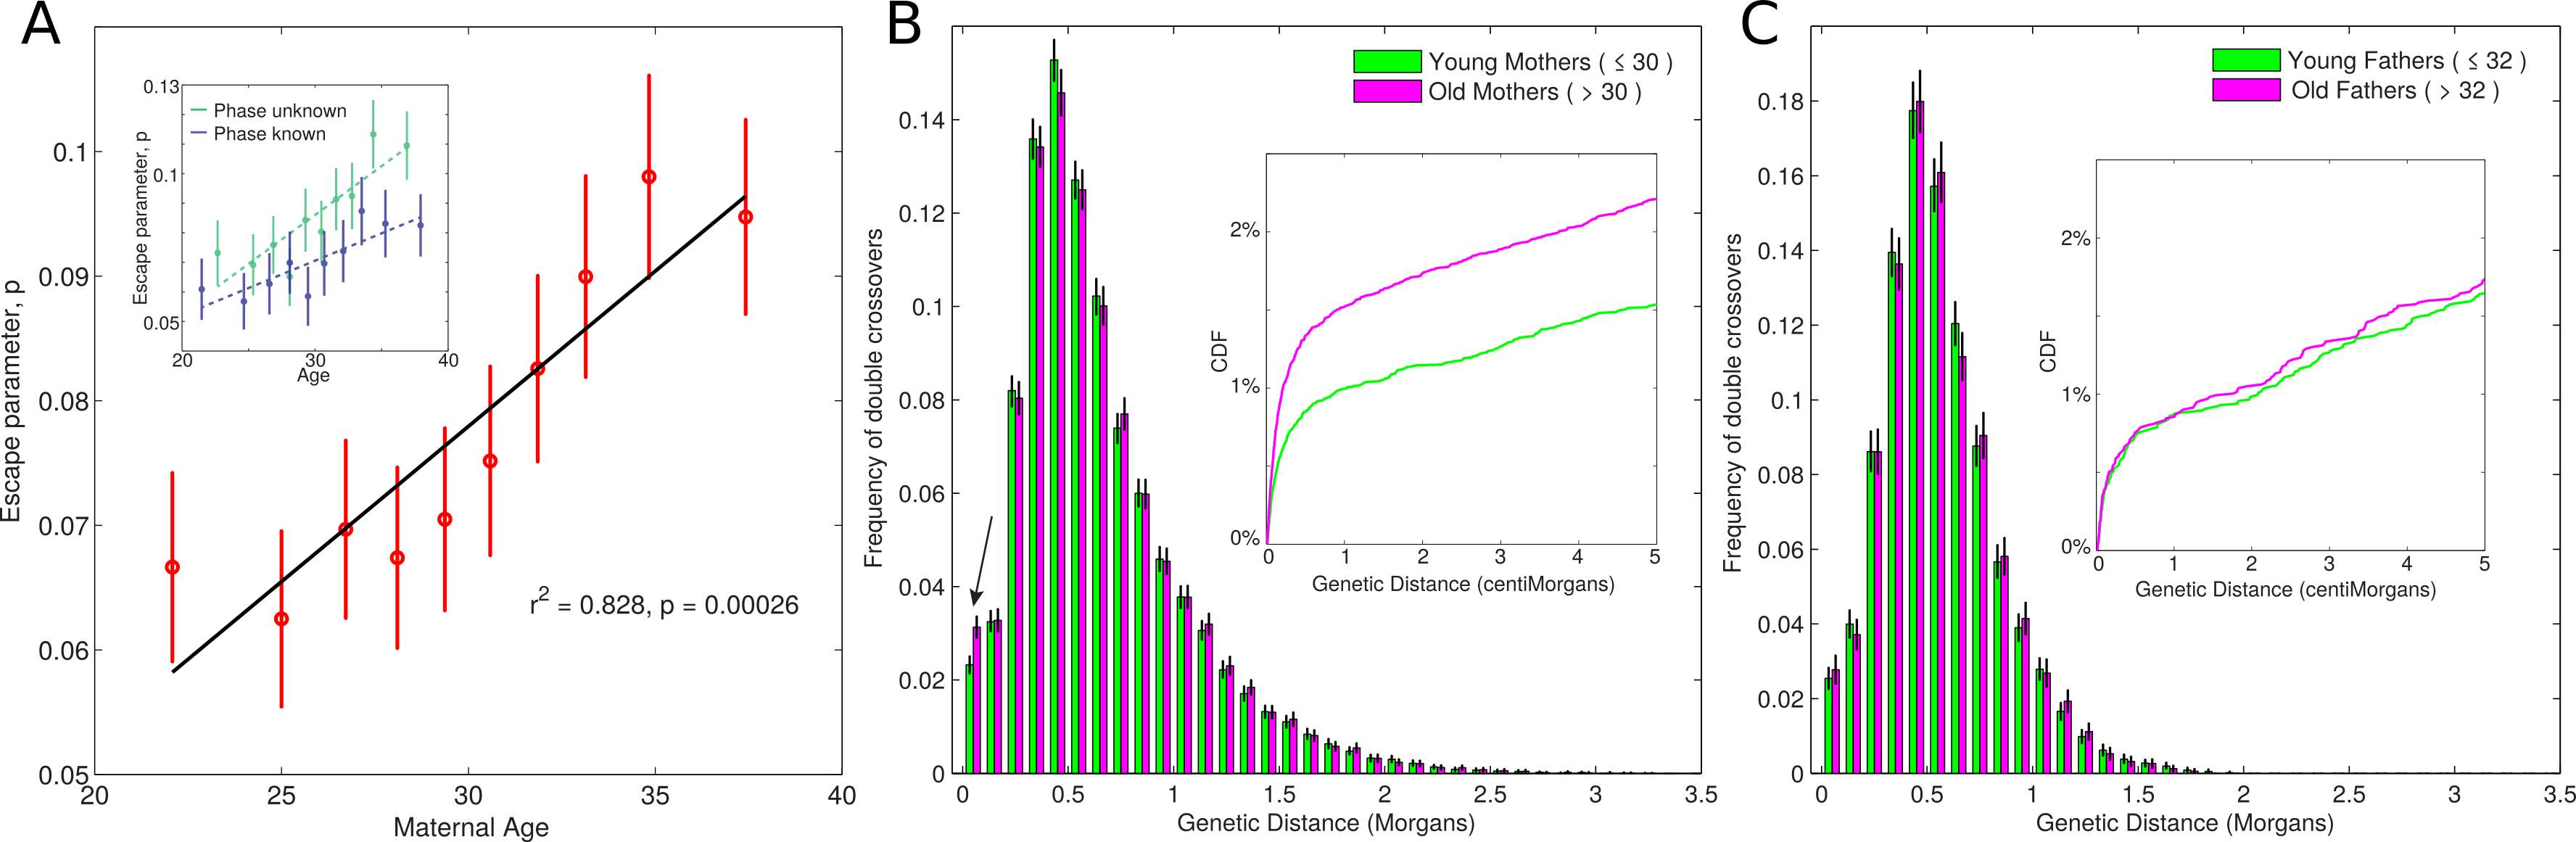
\includegraphics[width=\textwidth]{cointEscape/figs/Figure4.png}
    %\vspace{-20pt}
    \captionTitle{\textbf{Number of autosome recombination events verses parental age}}{
        for females (left) and males (right). 
        A linear least-squares fit is indicated by a black line.
        The least-squares fit equation given in the legend together with a p-value for the non-constant term.   
       \label{fig:cointFS6}}
\end{figure}

\begin{figure}[!h]
    %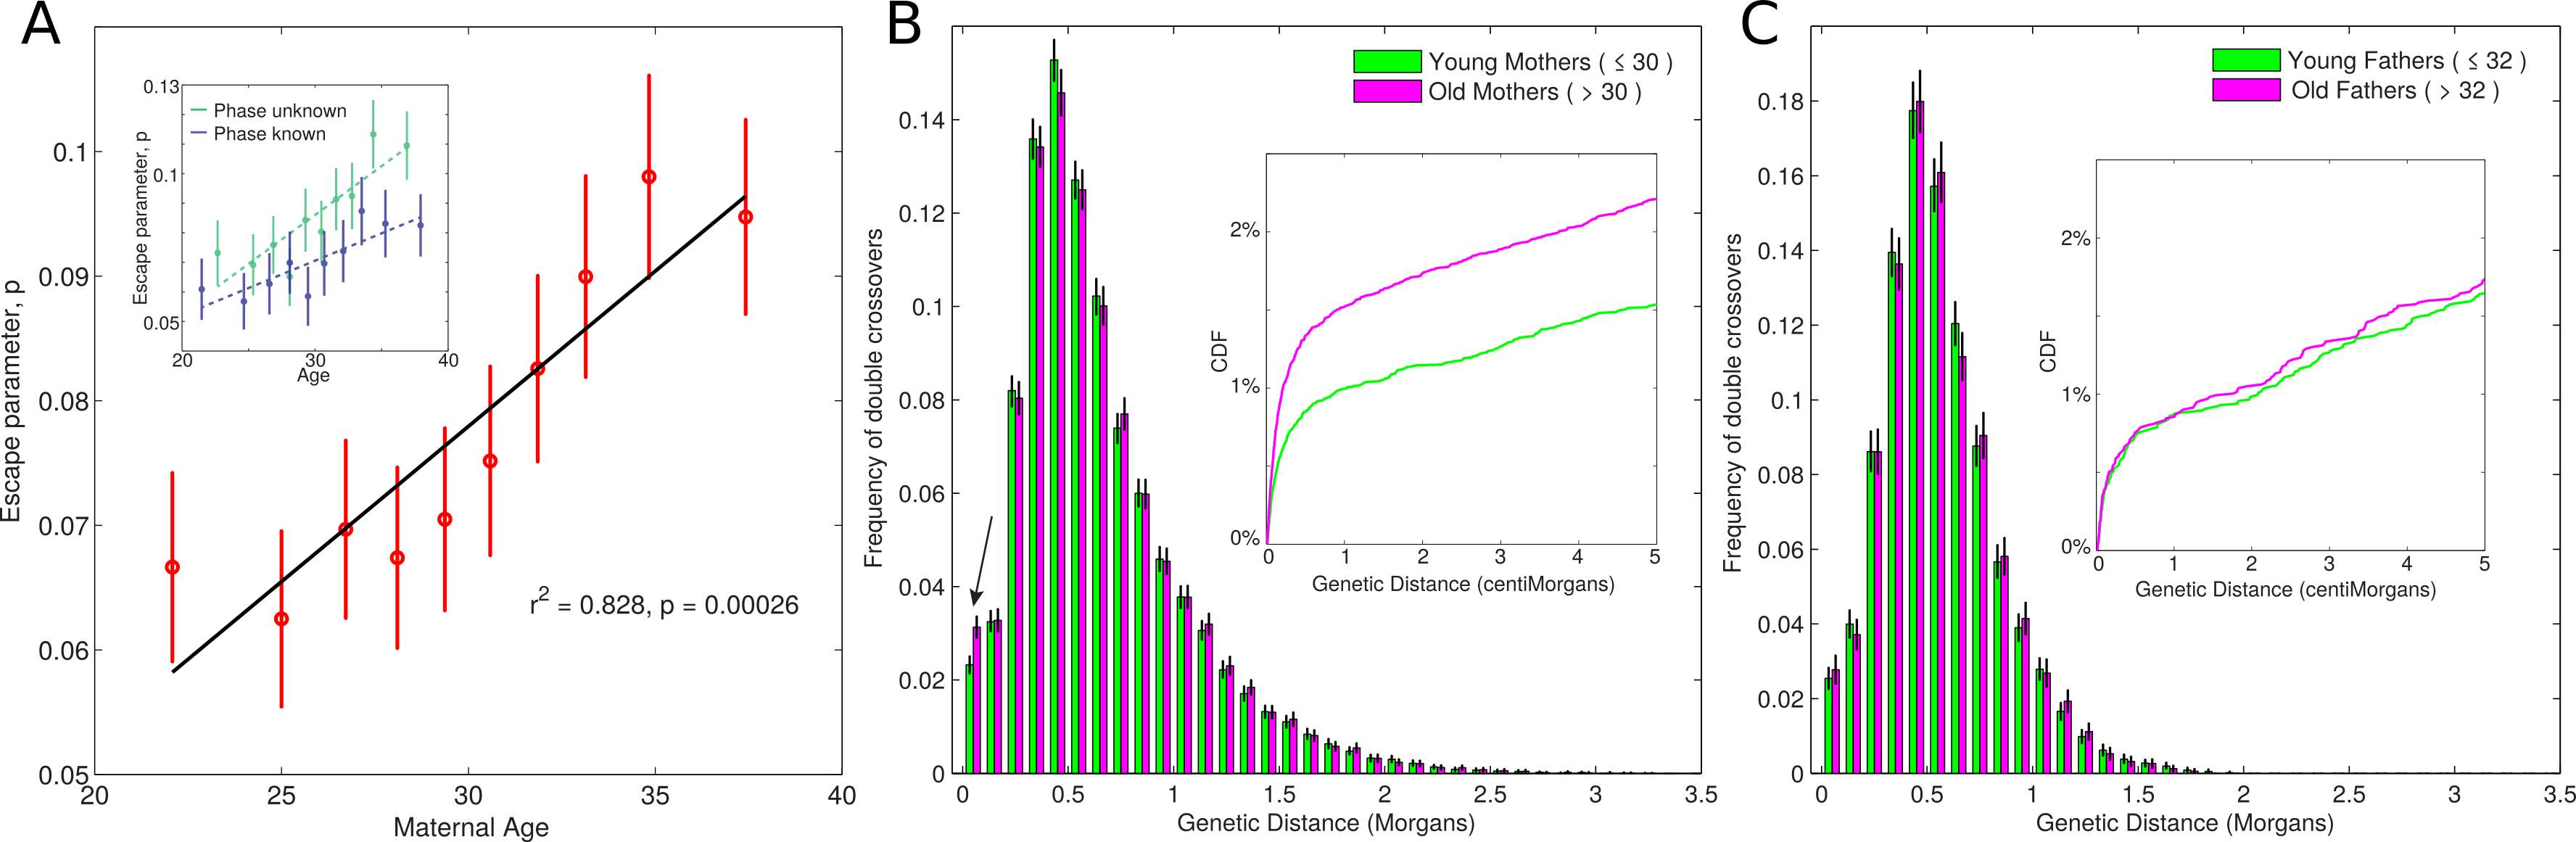
\includegraphics[width=\textwidth]{cointEscape/figs/Figure4.png}
    %\vspace{-20pt}
    \caption[\textbf{Hotspot usage between sexes.}]{
        A) Hotspot usage estimated in females (left) and males(right). 
        The MLE estimate for each individual is indicated by a circle, with a 95\% confidence interval indicated by the shaded area.
        The median MLE estimate for each sex is indicated by a vertical black line.
        B) Hotspot usage by parental age for females(left) and males (right).
        For each plot a logistic regression is also shown, with the p-value for the non-constant term given in the title.  
       \label{fig:cointFS7}}
\end{figure}

\begin{figure}[!h]
    %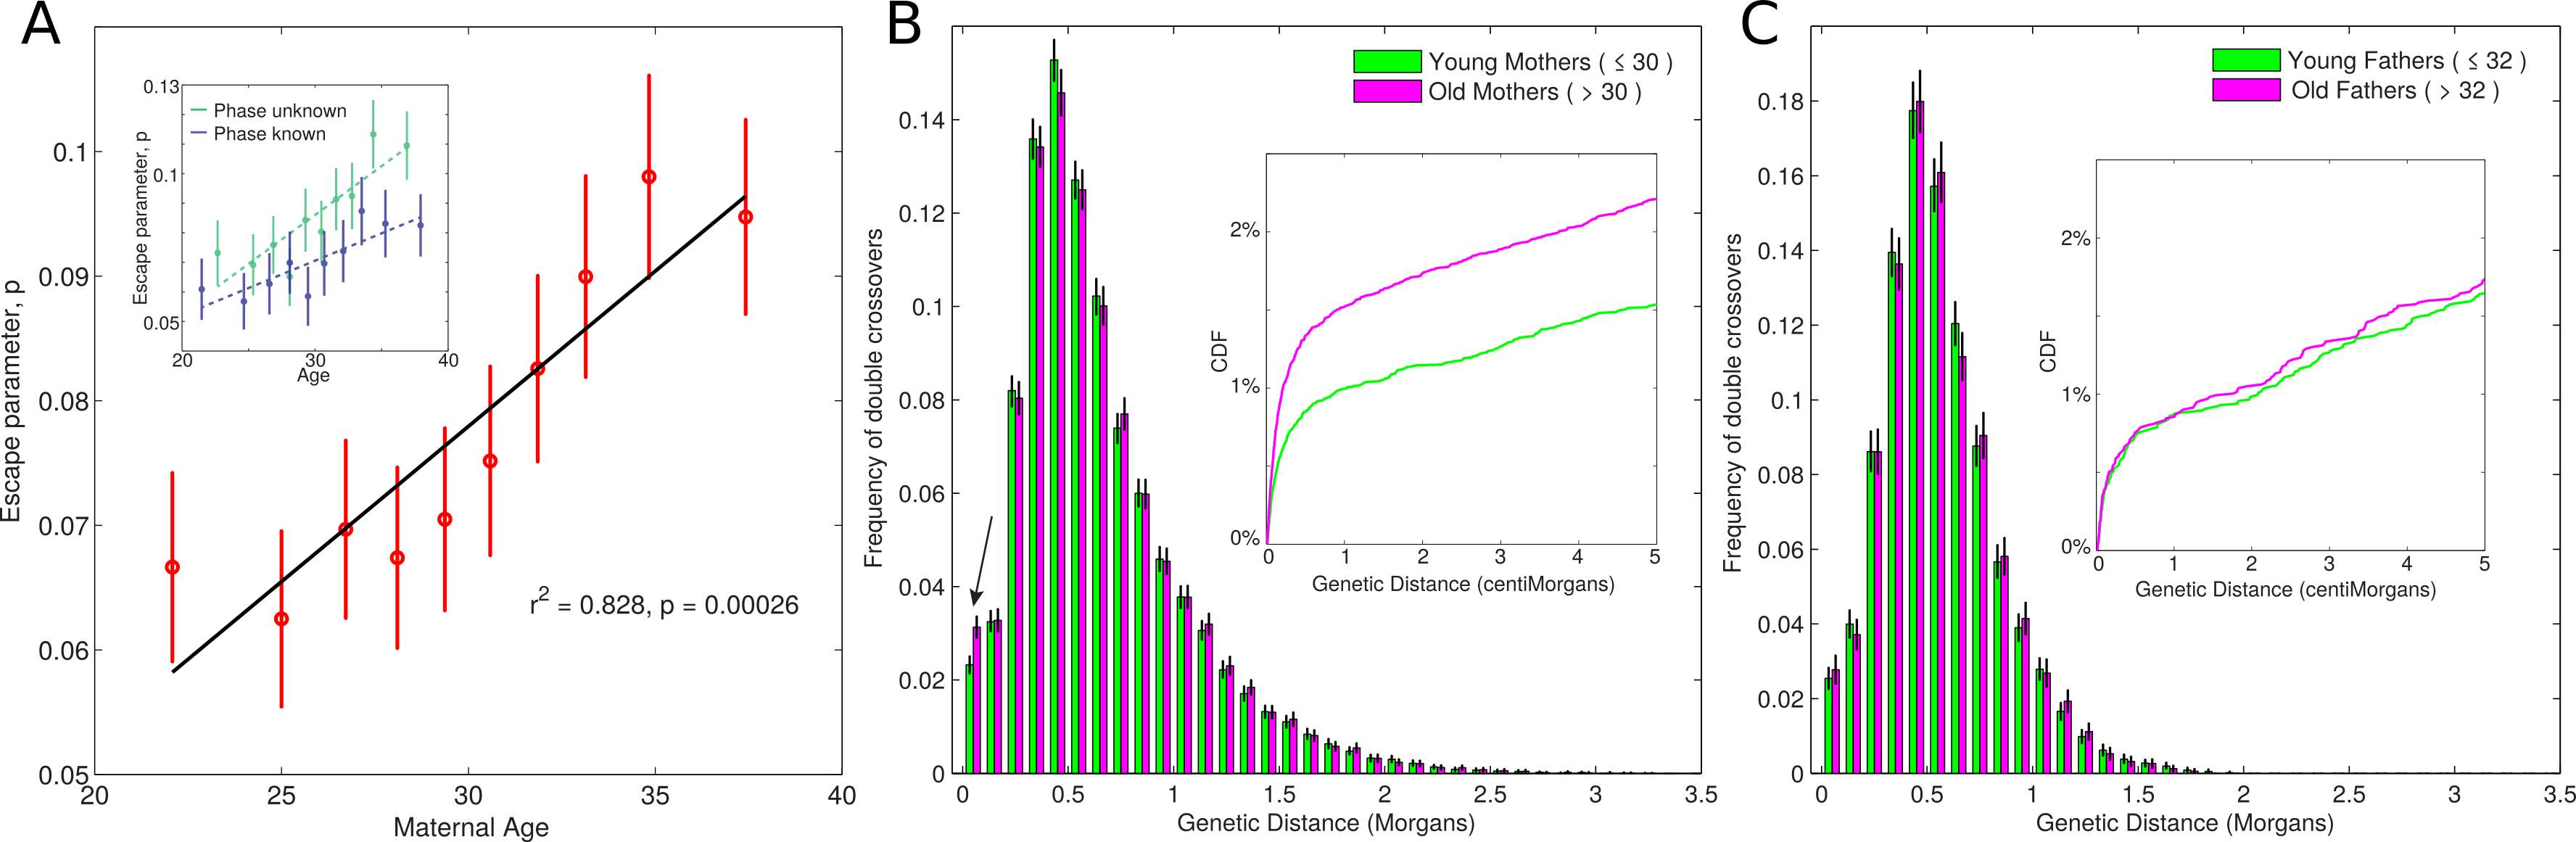
\includegraphics[width=\textwidth]{cointEscape/figs/Figure4.png}
    %\vspace{-20pt}
    \caption[\textbf{The relationship between map length and interference parameters.}]{ 
        A) The relationship between chromosome map length and the interference parameter, $\nu$.
        B) The relationship between chromosome map length and the escape parameter, $p$.
        Linear fits are shown for females (red), males (blue), and the data combined across sexes (black).
        In both plots, the chr21 estimate in males has been excluded.  
       \label{fig:cointFS8}}
\end{figure}

\begin{figure}[!h]
    %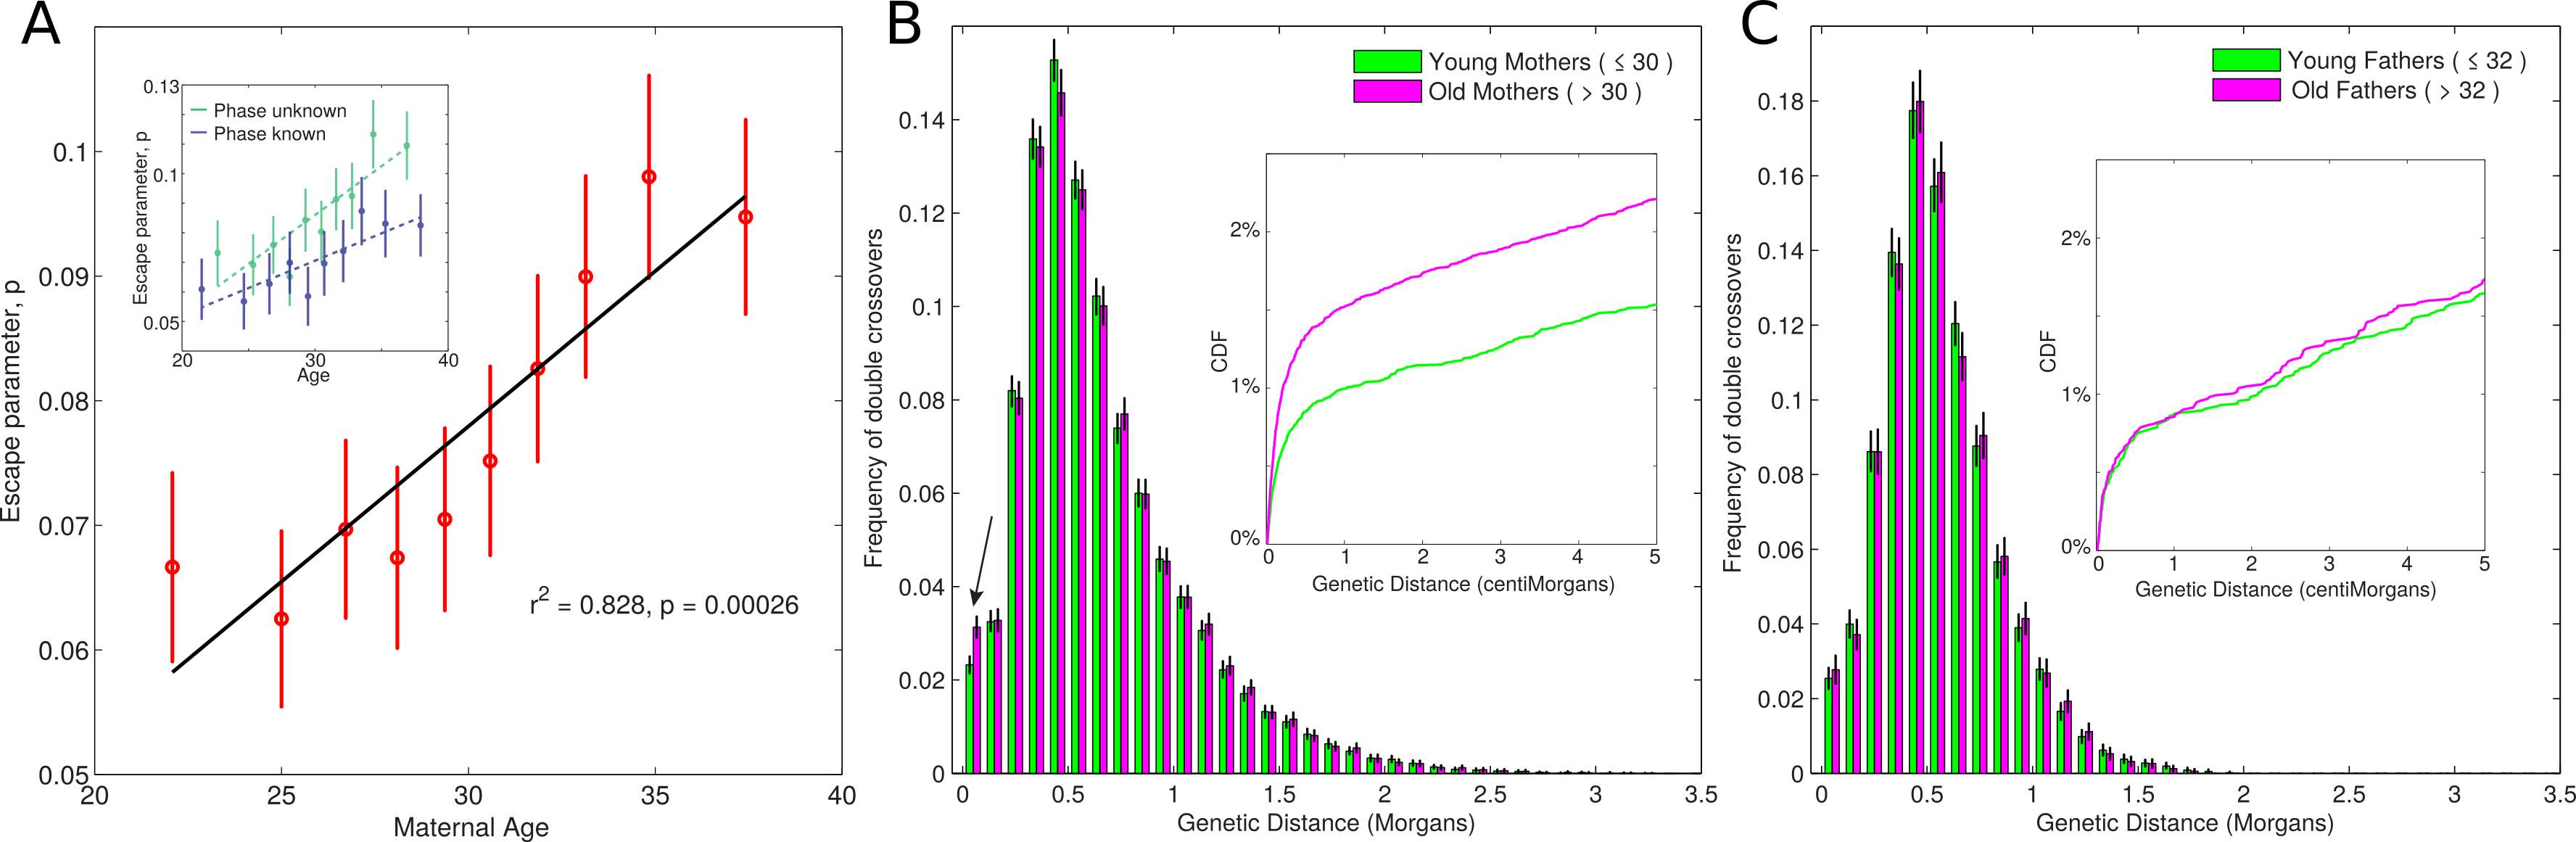
\includegraphics[width=\textwidth]{cointEscape/figs/Figure4.png}
    %\vspace{-20pt}
    \captionTitle{\textbf{Interference parameters as a function of age.}}{
        Females and males are shown on the top and bottom rows respectively. 
        Estimates of the interference parameter, $\nu$, are shown on the left, whereas estimates of the escape parameter, $p$, are shown on the right.
        Error bars show 95\% confidence intervals.  
       \label{fig:cointFS9}}
\end{figure}

\begin{figure}[!h]
    %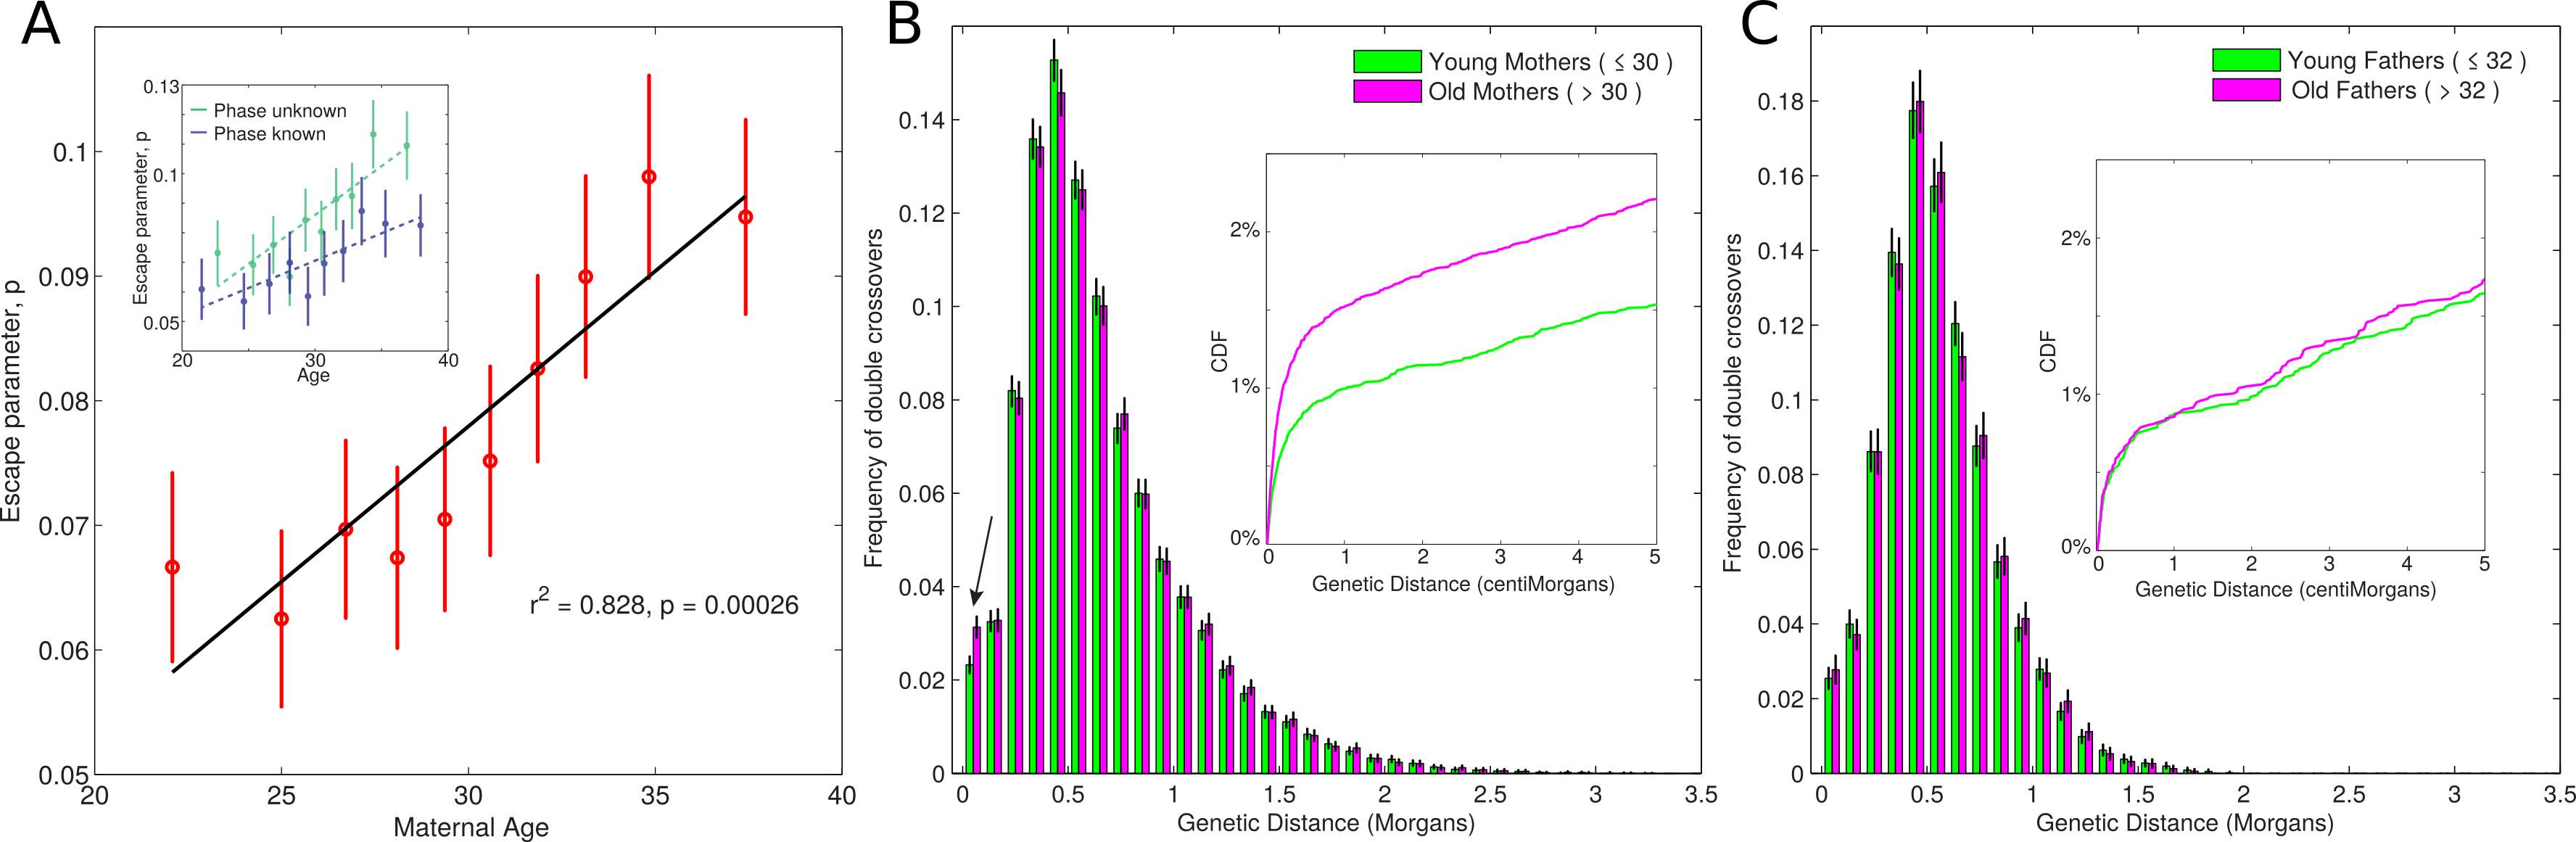
\includegraphics[width=\textwidth]{cointEscape/figs/Figure4.png}
    %\vspace{-20pt}
    \captionTitle{\textbf{Interference parameters by age}}{,
        having divided the data in 5 or 20 age quantiles.
        Error bars show 95\% confidence intervals.  
       \label{fig:cointFS10}}
\end{figure}

\begin{figure}[!h]
    %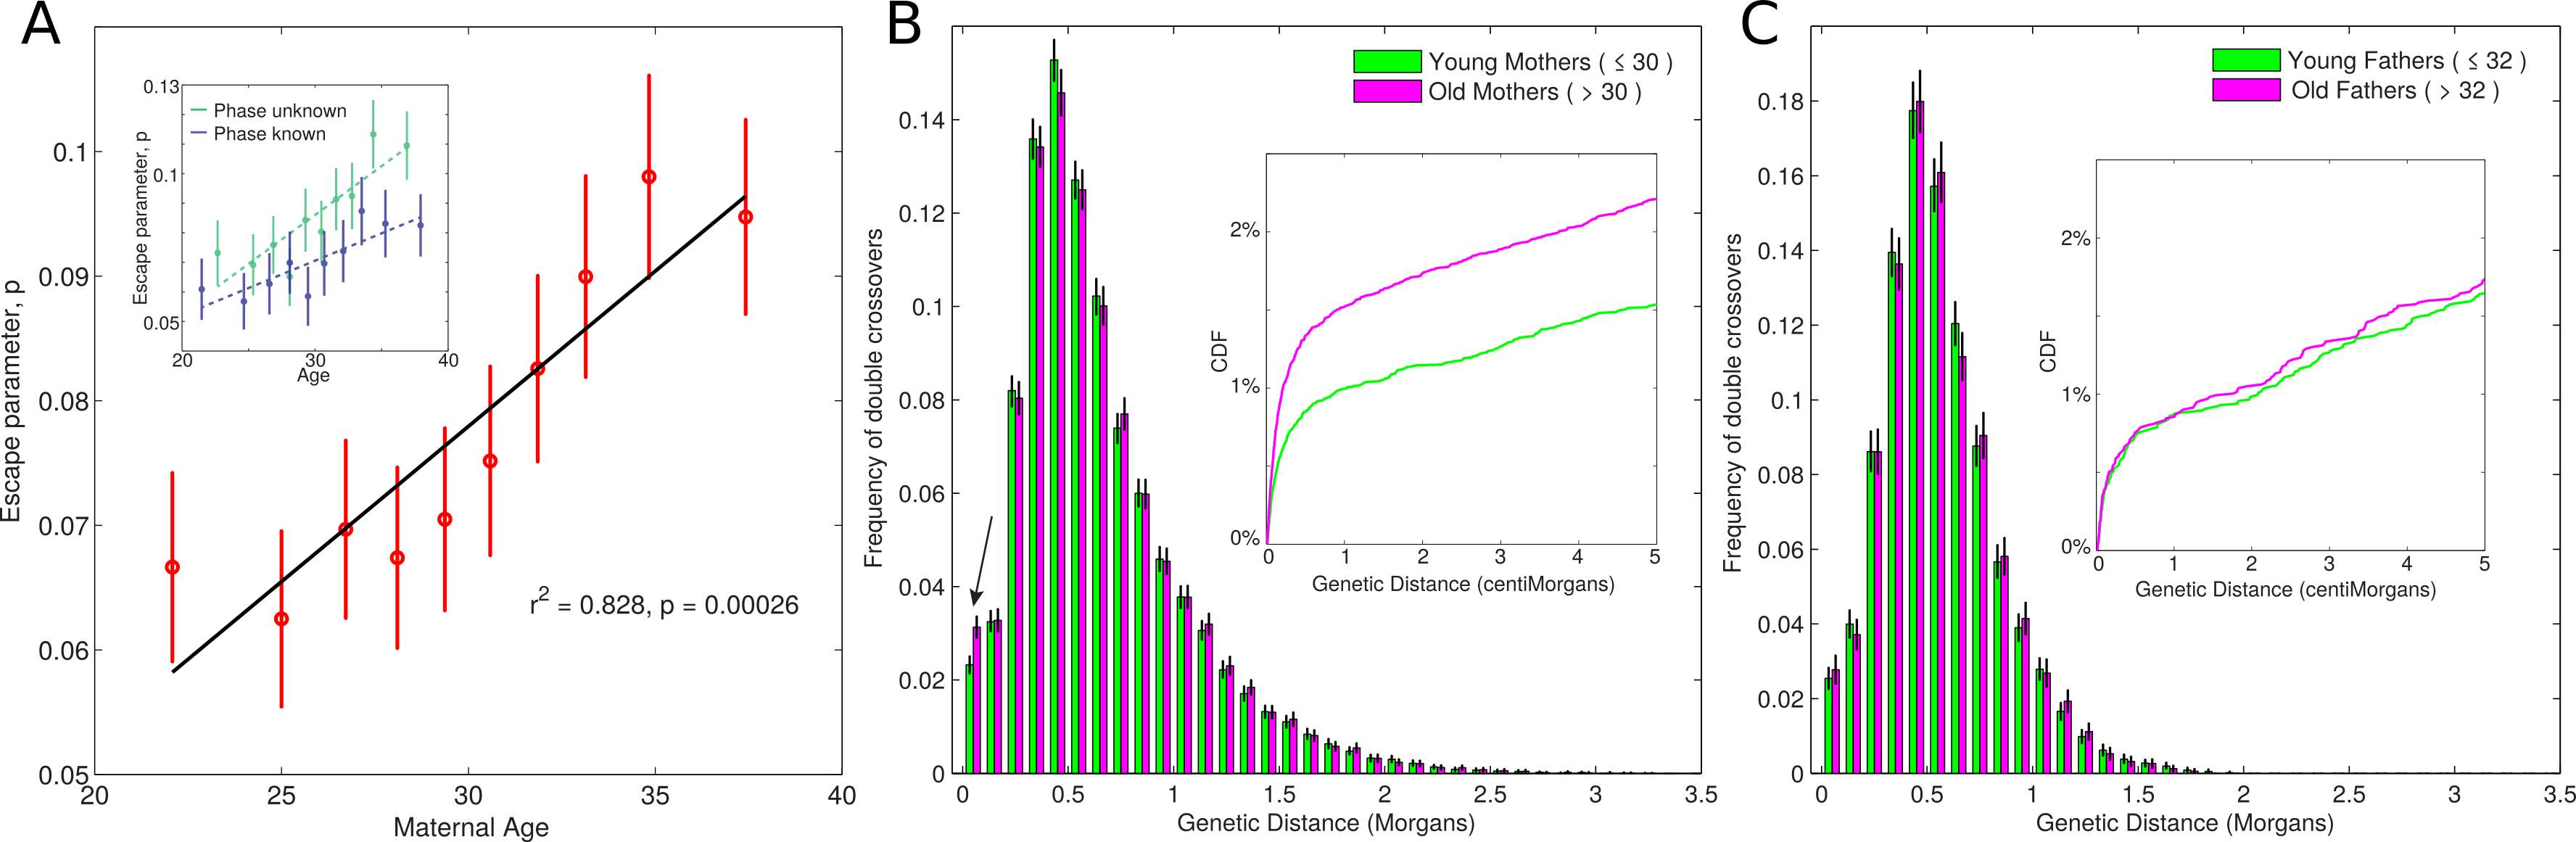
\includegraphics[width=\textwidth]{cointEscape/figs/Figure4.png}
    %\vspace{-20pt}
    \caption{\textbf{Interference parameters by age and phase.}}{ 
        Interference parameters by age, having estimated the interference parameters for phase-known and phase-unknown groups separately.  
       \label{fig:cointFS11}}
\end{figure}

\begin{figure}[!h]
    %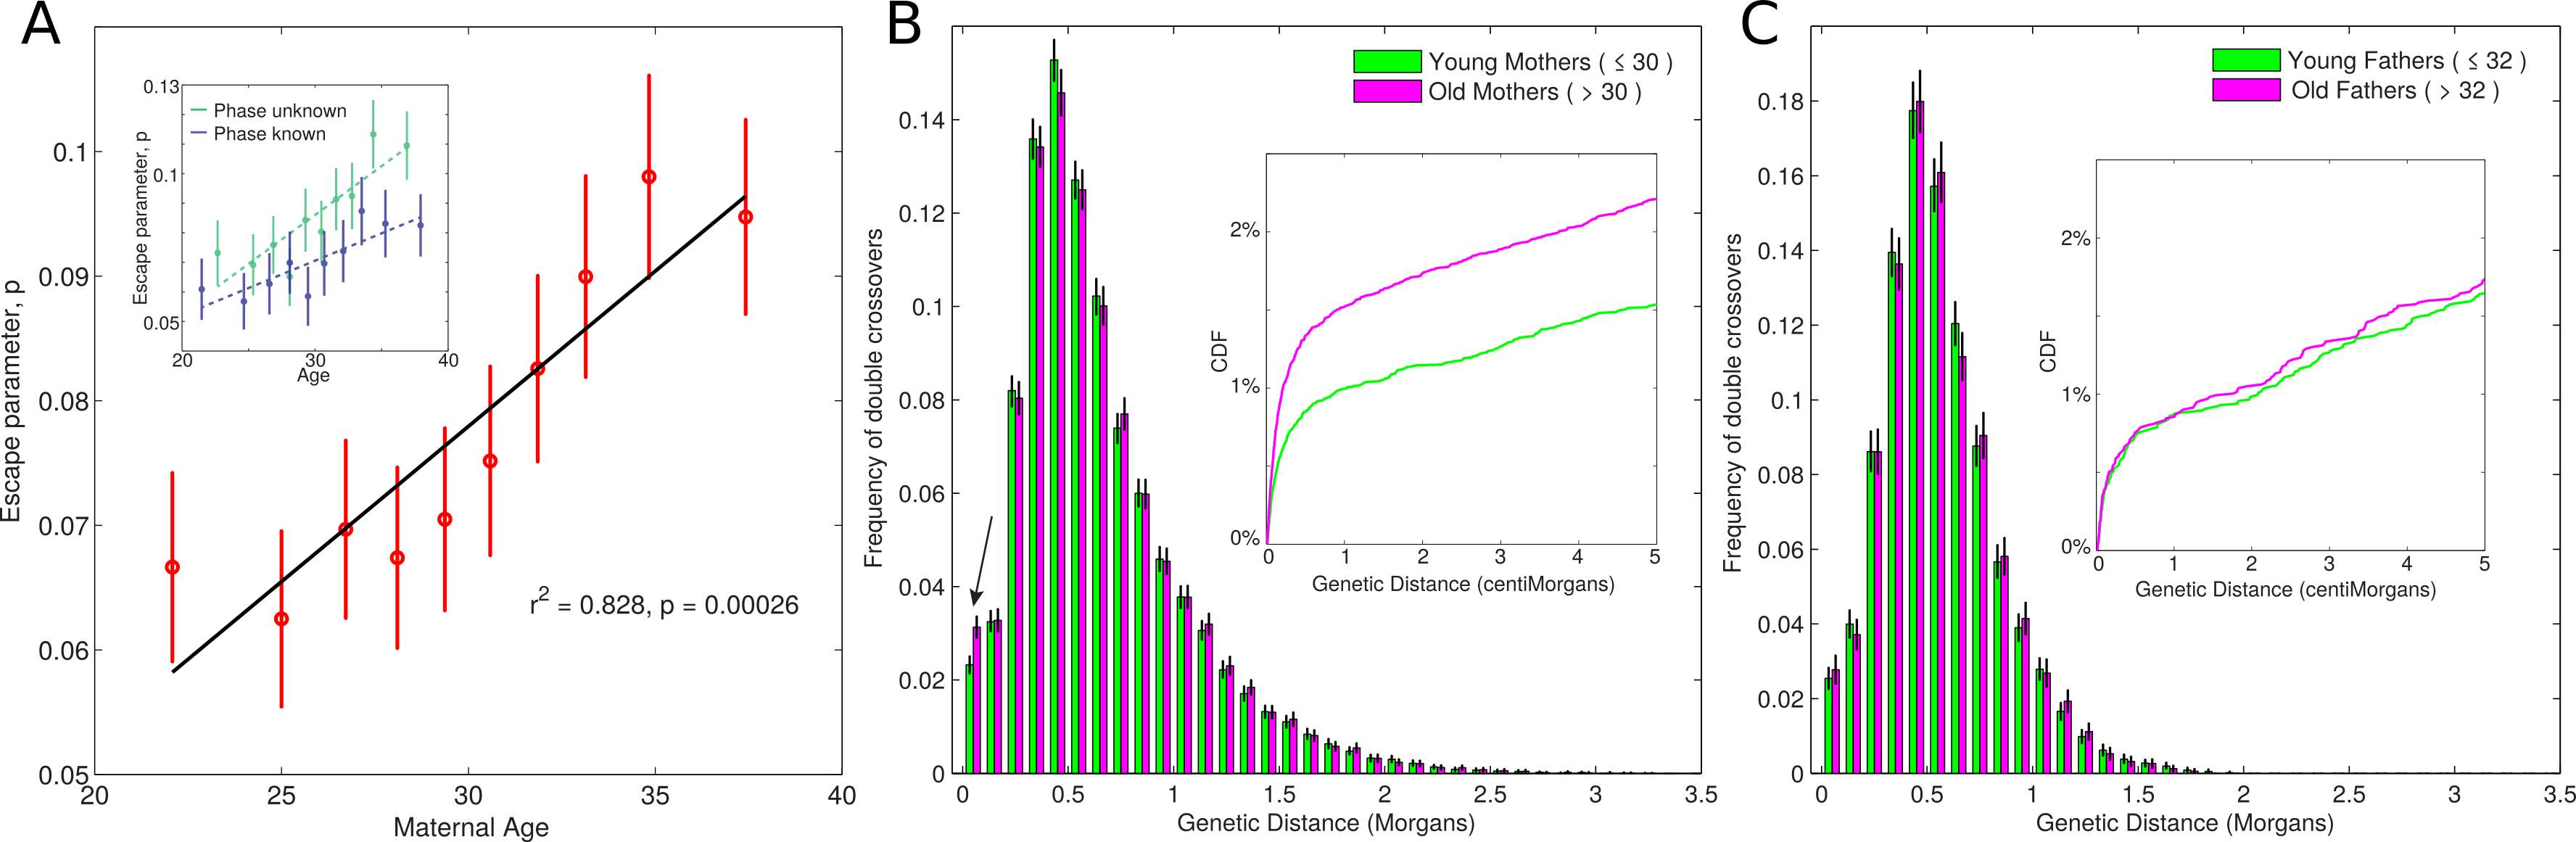
\includegraphics[width=\textwidth]{cointEscape/figs/Figure4.png}
    %\vspace{-20pt}
    \captionTitle{\textbf{Interference parameters as a function of age, following stratified sampling.}}{
        Females and males are shown on the top and bottom rows respectively.
        Estimates of the interference parameter, $\nu$, are shown on the left, whereas estimates of the escape parameter, $p$, are shown on the right.
        Error bars show 95\% confidence intervals.  
       \label{fig:cointFS12}}
\end{figure}

\begin{figure}[!h]
    %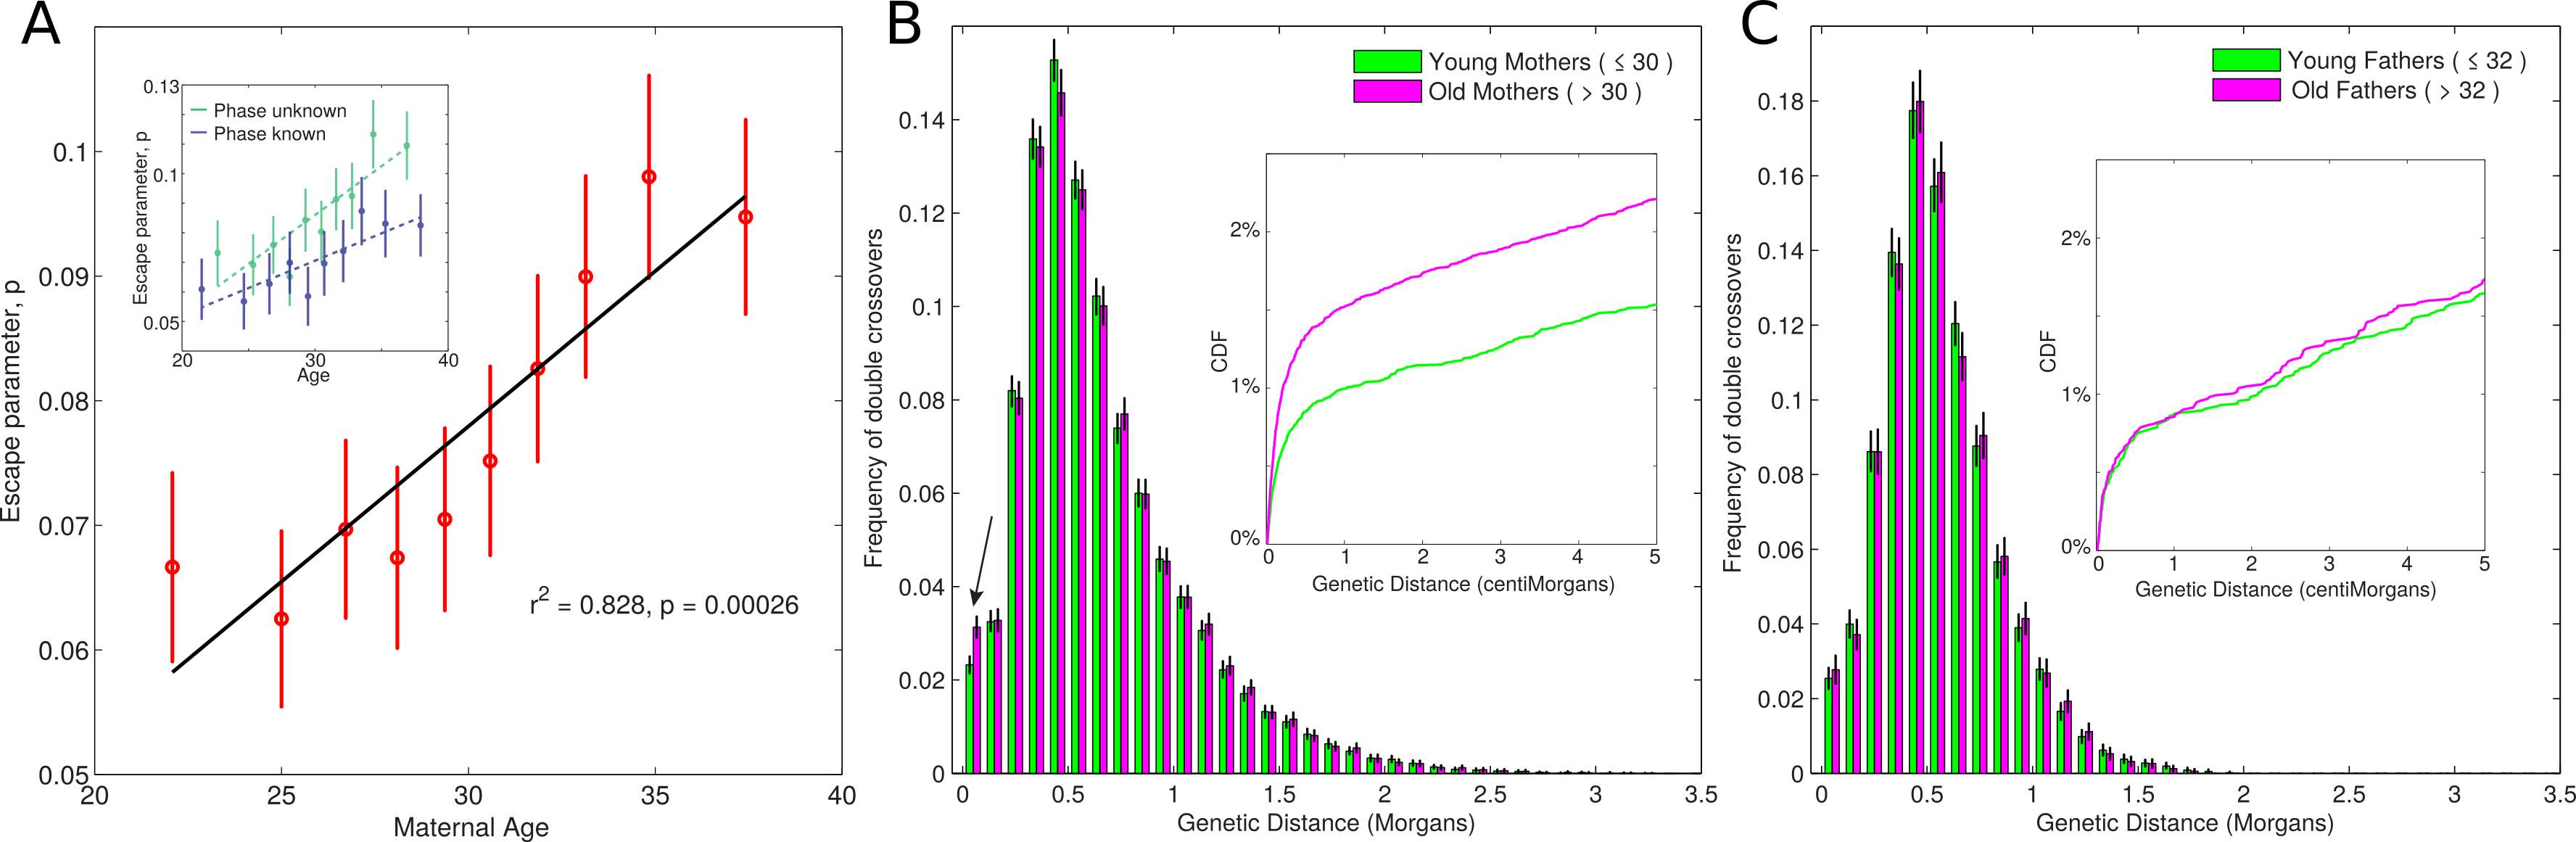
\includegraphics[width=\textwidth]{cointEscape/figs/Figure4.png}
    \vspace{-20pt}
    \captionTitle{\textbf{Model fit for tightly clustered events}}{
        in females (A) and males (B).
        The figure shows the empirical cumulative distribution function for young (green line) and old (magenta line) mothers/fathers, and compares to that obtained via simulation under the interference free model (black dotted line), the Gamma simple interference model (black dashed line), and the Housworth-Stahl interference escape model (solid black line), with parameters were taken from Supplementary Table 7.
        The figure is shown on a log-log scale to emphasize the short inter-crossover distances.  
       \label{fig:cointFS13}}
\end{figure}

\begin{figure}[!h]
    %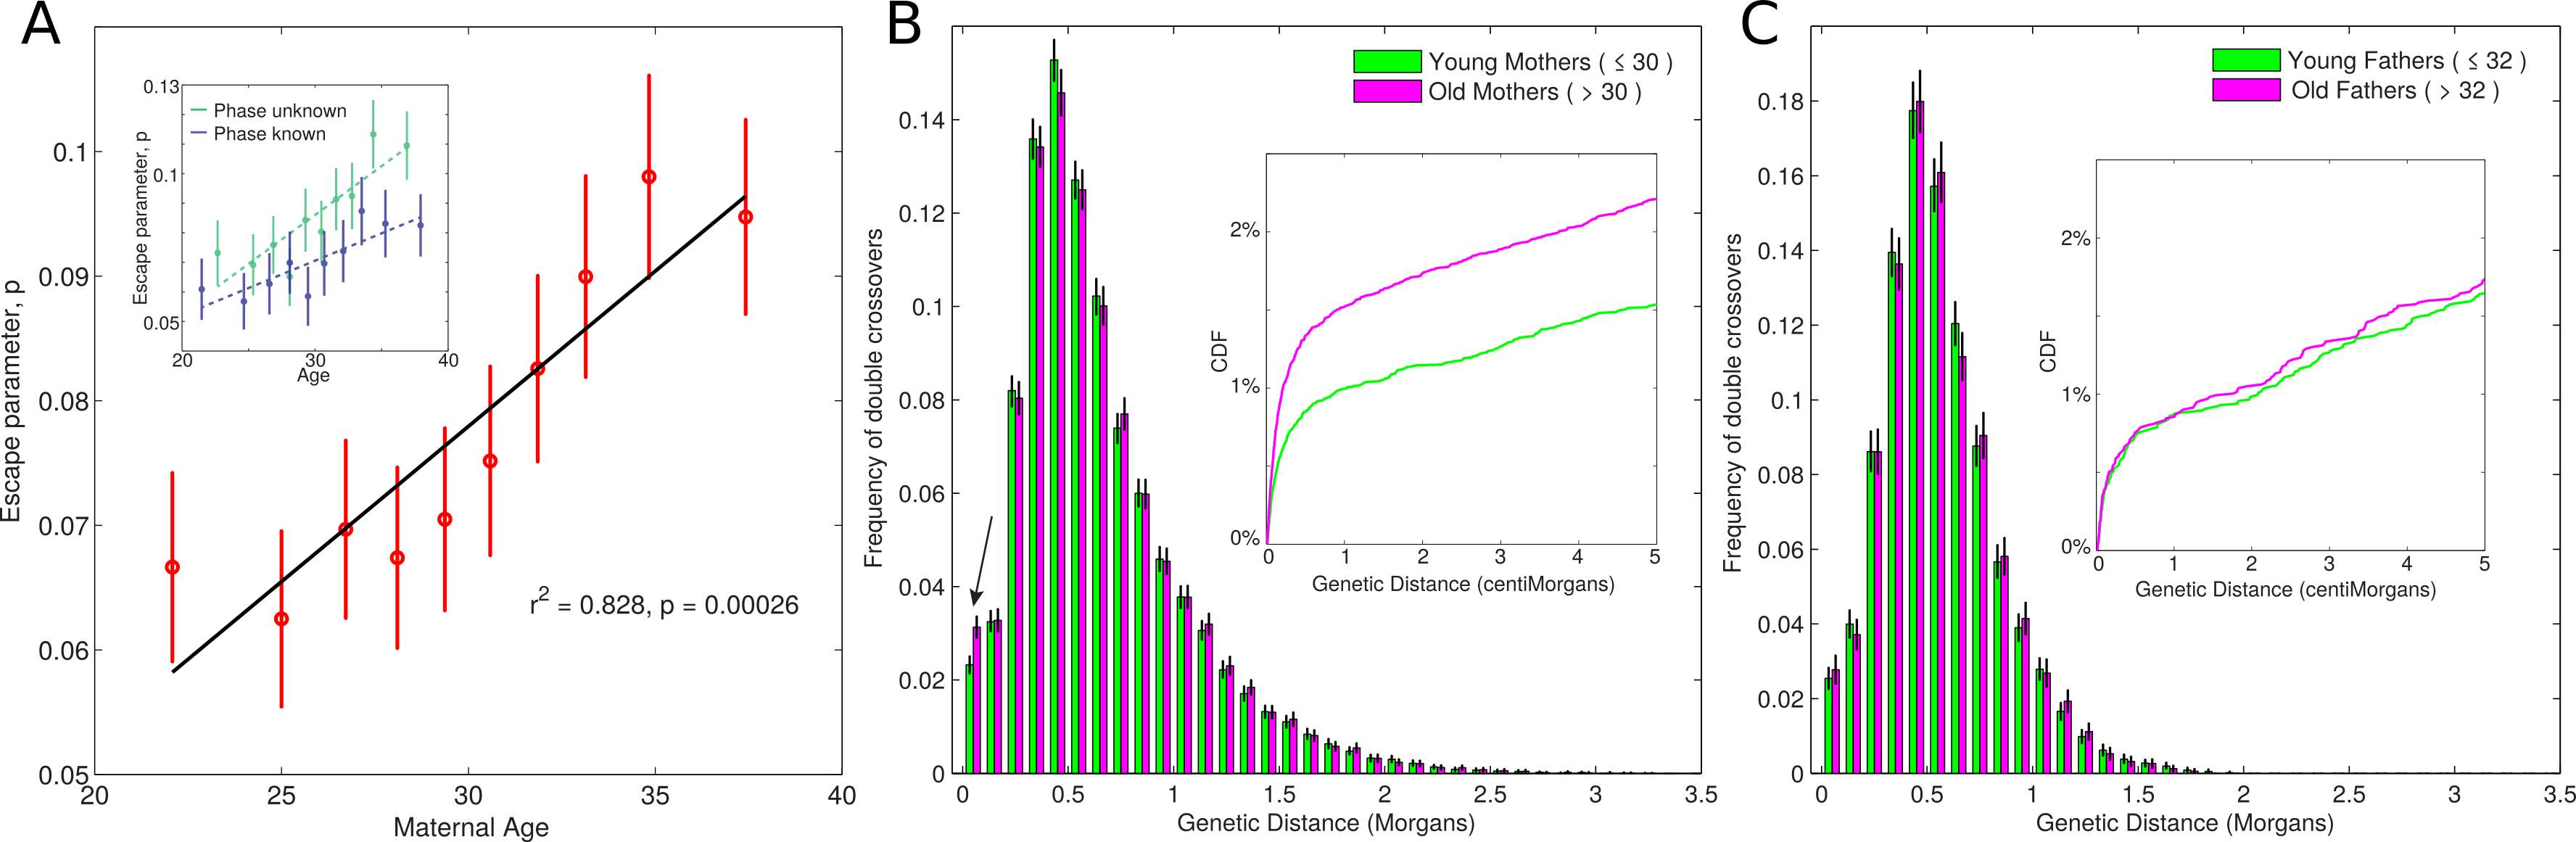
\includegraphics[width=\textwidth]{cointEscape/figs/Figure4.png}
    \vspace{-20pt}
    \captionTitle{\textbf{Interference parameters estimated for a strictly filtered dataset.}}{
        In this case, all crossover events were required at least 10 supporting informative sites (compared to 3 in the main dataset), no two events within a single family were allowed to be within 5 SNPs of each other (compared to 1 in the main dataset), and no more than 4 events within 1 Mb of each other were allowed across the whole dataset (and compared to 14 in the main dataset, which corresponds to the 99.9\textsuperscript{th} percentile).
        After this very strict filtering, the deviation from the Housworth-Stahl interference escape model is much less pronounced at short scales (right hand panels), but the association between interference escape and maternal  
        age remains strong (2\textsuperscript{nd} panel from top left).   
       \label{fig:cointFS14}}
\end{figure}


\subsection{Supplementary Tables}


\begin{table}[!h] \centering
    \begin{tabular}{|c|c|c|c|} 
        \hline Pedigree Type & Description & Before Filtering & After Filtering \\ \hline
        1 & 2 parents, 2 children & 3319 & 3307 \\
        2 & 2 parents, 3 children & 560 & 523 \\
        3 & 2 parents, 4 children & 89 & 80 \\
        4 & Quartet, with 2nd generation trio & 101 & 100 \\
        5 & Trio, with 2nd generation quartet & 201 & 199 \\
        \hline & \textbf{Total} & \textbf{4270} & \textbf{4209} \\
    \hline \end{tabular}
    \captionTitle{\textbf{Summary of dataset, before and after filtering.}}{
    \label{tab:cointTS1}}
\end{table}

\begin{table}[!h] \centering
    \begin{tabular}{|p{3cm}p{1.5cm}p{1.5cm}p{1.5cm}p{1.5cm}p{1.5cm}p{2cm}|}
        \hline 
    Population & Female \mbox{unphased} & Male \mbox{unphased} & Female phased & Male phased & Total Meioses & Percentage \\ \hline
    Europe & 5382 & 5508 & 1789 & 1641 & 14320 & 78.24\% \\
    Latino & 602 & 546 & 171 & 190 & 1509 & 8.25\% \\
    East Asia & 380 & 308 & 88 & 74 & 850 & 4.64\% \\
    None/Other & 198 & 268 & 68 & 109 & 643 & 3.51\% \\
    South Asia & 178 & 176 & 19 & 20 & 393 & 2.15\% \\
    African American & 152 & 152 & 34 & 36 & 374 & 2.04\% \\
    Middle East & 76 & 100 & 15 & 22 & 213 & 1.16\% \\
    \hline \textbf{Total} & \textbf{6968} & \textbf{7058} & \textbf{2184} & \textbf{2092} & \textbf{18302} & \textbf{100.00\%} \\
    \hline \end{tabular}
    \captionTitle{\textbf{Description of parental ancestry for each meiosis within the sample.}} {
    \label{tab:cointTS2}}
\end{table}

\begin{table}[!h] \centering
    \footnotesize
    \begin{tabular}{|cp{1.2cm}p{1.4cm}p{1.1cm}p{1.1cm}p{1.0cm}p{1.1cm}p{1.0cm}p{1.1cm}p{1.0cm}|}
        \hline 
Chrom & First Position (bp) & Last Position (bp) & Physical Length (Mb) & Female Map Length (cM) & Female Mean Rate (cM/Mb) & Male Map Length (cM) & Male Mean Rate (cM/Mb) & SexAvg Map Length (cM) & SexAvg Mean Rate (cM/Mb) \\ \hline
chr1 & 1,031,540 & 249,170,711 & 248.14 & 335.9 & 1.36 & 198.30 & 0.80 & 267.05 & 1.08 \\
chr2 & 118,913 & 242,763,542 & 242.64 & 316.45 & 1.31 & 184.64 & 0.76 & 250.52 & 1.03 \\
chr3 & 152,592 & 197,759,785 & 197.61 & 270.98 & 1.37 & 163.85 & 0.83 & 217.4 & 1.1 \\
chr4 & 167,596 & 190,787,660 & 190.62 & 260.11 & 1.37 & 145.79 & 0.76 & 202.93 & 1.06 \\
chr5 & 184,702 & 180,673,228 & 180.49 & 249.13 & 1.38 & 146.66 & 0.81 & 197.87 & 1.1 \\
chr6 & 188,937 & 170,777,087 & 170.59 & 236.64 & 1.39 & 140.88 & 0.83 & 188.74 & 1.11 \\
chr7 & 67,365 & 159,042,351 & 158.97 & 223.17 & 1.41 & 136.04 & 0.86 & 179.55 & 1.13 \\
chr8 & 200,898 & 146,235,564 & 146.03 & 210.94 & 1.45 & 122.41 & 0.84 & 166.64 & 1.14 \\
chr9 & 215,269 & 141,004,945 & 140.79 & 195.69 & 1.4 & 125.54 & 0.89 & 160.58 & 1.14 \\
chr10 & 162,102 & 135,402,200 & 135.24 & 207.86 & 1.54 & 129.91 & 0.96 & 168.86 & 1.25 \\
chr11 & 244,552 & 134,872,342 & 134.63 & 193.59 & 1.44 & 120.21 & 0.89 & 156.88 & 1.17 \\
chr12 & 216,039 & 133,684,321 & 133.47 & 200.36 & 1.51 & 131.20 & 0.98 & 165.75 & 1.24 \\
chr13 & 19,458,371 & 114,998,076 & 95.54 & 152.26 & 1.6 & 101.19 & 1.06 & 126.71 & 1.33 \\
chr14 & 20,445,905 & 107,233,999 & 86.79 & 137.22 & 1.59 & 97.29 & 1.12 & 117.24 & 1.35 \\
chr15 & 22,763,396 & 102,381,360 & 79.62 & 143.39 & 1.8 & 100.85 & 1.27 & 122.11 & 1.53 \\
chr16 & 143,503 & 90,102,384 & 89.96 & 157.29 & 1.75 & 102.03 & 1.13 & 129.64 & 1.44 \\
chr17 & 84,782 & 81,025,393 & 80.94 & 152.87 & 1.9 & 106.23 & 1.31 & 129.53 & 1.6 \\
chr18 & 218,695 & 77,955,378 & 77.74 & 140.06 & 1.81 & 97.80 & 1.26 & 118.91 & 1.53 \\
chr19 & 288,246 & 59,058,083 & 58.77 & 117.8 & 2.01 & 99.42 & 1.69 & 108.59 & 1.85 \\
chr20 & 100,699 & 62,892,739 & 62.79 & 118.9 & 1.9 & 99.00 & 1.58 & 108.93 & 1.73 \\
chr21 & 14,807,136 & 47,978,421 & 33.17 & 74.34 & 2.24 & 51.76 & 1.58 & 63.04 & 1.9 \\
chr22 & 17,152,611 & 51,165,664 & 34.01 & 78.16 & 2.31 & 63.30 & 1.86 & 70.71 & 2.08 \\
chrX & 2,737,282 & 154,408,041 & 151.67 & 179.02 & 1.18 &  &  &  &  \\
PAR1 & 178,624 & 2,689,575 & 2.51 & 2.73 & 1.16 & 42.94 & 17.17 & 22.75 & 9.06 \\
PAR2 & 154,984,651 & 155,227,607 & 0.24 & 0.05 & 0.34 & 0.33 & 1.35 & 0.19 & 0.79 \\
        \hline Genome &&& 2932.98 & 4354.91 & 1.48 & 2707.55 & 0.92 & 3441.11 & 1.17 \\
    \hline \end{tabular}
    \captionTitle{\textbf{Properties of the map estimated from 23andMe data.}}{
        Recombination fractions were converted to genetic map distances using the Haldane map function.  
    \label{tab:cointTS3}}
\end{table}

\begin{table}[!h] \centering
    \footnotesize
    \begin{tabular}{|cccccccc|}
        \hline 
SNP & Chrom & Position & Alleles & P-value & Effect & 95\% CI & Gene Context \\ \hline
rs2001572 & chr14 & 20,767,868 & A/T & 1.50E-08 & 0.503 & [0.329,0.677] & [TTC5] \\
rs79621814 & chr4 & 1,089,268 & C/T & 2.90E-08 & -0.99 & [-1.340,-0.640] & [RNF212] \\
rs11624006 & chr14 & 91,961,188 & C/T & 2.80E-07 & -0.478 & [-0.660,-0.296] & [SMEK1] \\
rs72631326 & chr17 & 65,769,087 & C/T & 4.40E-07 & 0.959 & [0.587,1.331] & NOL11--[]--BPTF \\
rs11932663 & chr4 & 184,458,083 & A/G & 5.10E-07 & 0.622 & [0.380,0.865] & ING2--[]---RWDD4 \\
rs17127442 & chr8 & 18,779,787 & C/T & 5.10E-07 & -0.537 & [-0.746,-0.327] & [PSD3] \\
rs1879904 & chr11 & 82,076,387 & C/T & 6.80E-07 & -0.507 & [-0.707,-0.307] & []---FAM181B \\
    \hline \end{tabular}
    \captionTitle{\textbf{Variants associated with total number of recombination events.}}{
        Linear regression model tested as N\_events $\sim$ sex + age + pc.0 + pc.1 + pc.2 + pc.3 + pc.4 + genotype. 
        Association tests conducted using only individuals found to have $\ge$ 97\% European ancestry. 
    \label{tab:cointTS4}}
\end{table}

\clearpage 

\begin{table}[!h] \centering
    \footnotesize
    \begin{tabular}{|cccccccc|}
        \hline 
SNP & Chrom & Position & Alleles & P-value & Effect & 95\% CI & Gene Context \\ \hline
rs73742307 & chr5 & 23,534,421 & C/T & 7.90E-184 & 0.16 & [0.149,0.170] & PRDM9-[]---CDH10 \\
rs78474856 & chr20 & 1,450,623 & C/G & 6.10E-07 & -0.021 & [-0.029,-0.013] & NSFL1C-[]-SIRPB2 \\
rs62078596 & chr17 & 53,906,496 & C/T & 8.50E-07 & 0.013 & [0.008,0.018] & PCTP--[]---ANKFN1 \\
rs8134126 & chr21 & 28,401,705 & C/T & 1.00E-06 & -0.01 & [-0.013,-0.006] & ADAMTS5--[] \\
rs138108783 & chr1 & 119,711,419 & A/G & 1.40E-06 & 0.274 & [0.163,0.385] & WARS2--[]---HAO2 \\
    \hline \end{tabular}
    \captionTitle{\textbf{Variants associated with hotspot usage.}}{
        Linear regression model tested as hotspot\_usage $\sim$ sex + age + pc.0 + pc.1 + pc.2 + pc.3 + pc.4 + genotype.
        Association tests conducted using only individuals found to have $\ge$ 97\% European ancestry.  
    \label{tab:cointTS5}}
\end{table}

\begin{table}[!h] \centering
    %\footnotesize
    \begin{tabular}{|cp{1.5cm}p{1.5cm}p{1.5cm}p{1.5cm}cp{2cm}|}
        \hline 
        Population & Female sample size* & Male sample size* & Female median hotspot usage & Male median hotspot usage & Difference & p-value (Mann-Whitney U) \\ \hline
        Europe & 3329 & 3325 & 62.96\% & 67.12\% & 4.16\% & 4.93E-40 \\
        Latino & 362 & 341 & 61.15\% & 66.84\% & 5.68\% & 1.36E-09 \\
        East Asia & 221 & 180 & 60.38\% & 67.56\% & 7.18\% & 5.67E-06 \\
        South Asia & 97 & 95 & 61.65\% & 66.35\% & 4.71\% & 0.00494563 \\
        Middle East & 88 & 88 & 59.52\% & 61.26\% & 1.74\% & 0.284789 \\
        African American & 43 & 57 & 61.37\% & 65.37\% & 4.00\% & 0.135323 \\
        \hline All & 5668 & 5621 & 0.6268 & 0.67255 & 0.04575 & 1.06E-69 \\
    \hline \end{tabular}
\captionTitle{\textbf{Differences in hotspot usage between males and females}}{, partitioned by population.
        *The sample size represents the number estimated $\alpha$s, with one estimate for each meiosis from phase-known parents, and a single estimate for phase-unknown parents.  
    \label{tab:cointTS6}}
\end{table}

\clearpage 
\begin{table}[!h] \centering
    \scriptsize
    \begin{tabular}{|c|p{1.1cm}p{1.2cm}p{1.3cm}|cccccc|} \hline 
    \multicolumn{10}{|l|}{\textbf{Females}} \\ \hline
    & \multicolumn{3}{c|}{\textbf{Gamma model (no escape)}} & \multicolumn{6}{c|}{\textbf{Escape model}} \\
    & Phase known & Phase \mbox{unknown} & Weighted mean & 
    \multicolumn{2}{c}{Phase known} & \multicolumn{2}{c}{Phase unknown} & \multicolumn{2}{c|}{Weighted mean} \\
    Chrom & $\nu$ & $\nu$ & $\nu$ & $\nu$ & p & $\nu$ & p & $\nu$ & p \\ \hline
    chr1 & 2.749 & 3.211 & 2.952 & 6.045 & 0.067 & 6.711 & 0.079 & 6.384 & 0.073 \\
    chr2 & 2.390 & 3.035 & 2.643 & 6.499 & 0.064 & 6.902 & 0.076 & 6.718 & 0.070 \\
    chr3 & 2.328 & 2.653 & 2.473 & 6.489 & 0.072 & 6.612 & 0.089 & 6.556 & 0.081 \\
    chr4 & 3.074 & 3.956 & 3.414 & 5.981 & 0.042 & 6.036 & 0.047 & 6.009 & 0.044 \\
    chr5 & 3.289 & 3.824 & 3.526 & 6.582 & 0.044 & 6.941 & 0.065 & 6.753 & 0.052 \\
    chr6 & 2.893 & 2.864 & 2.878 & 7.221 & 0.055 & 7.395 & 0.086 & 7.314 & 0.069 \\
    chr7 & 3.007 & 2.826 & 2.902 & 7.435 & 0.048 & 7.289 & 0.090 & 7.360 & 0.065 \\
    chr8 & 1.395 & 2.014 & 1.566 & 8.073 & 0.165 & 6.615 & 0.184 & 7.141 & 0.175 \\
    chr9 & 1.760 & 2.590 & 2.007 & 6.168 & 0.095 & 7.096 & 0.113 & 6.586 & 0.105 \\
    chr10 & 2.548 & 4.228 & 2.971 & 7.561 & 0.066 & 7.039 & 0.056 & 7.260 & 0.061 \\
    chr11 & 2.485 & 2.829 & 2.645 & 7.466 & 0.065 & 8.240 & 0.084 & 7.818 & 0.074 \\
    chr12 & 2.979 & 3.896 & 3.323 & 7.519 & 0.058 & 6.927 & 0.060 & 7.175 & 0.059 \\
    chr13 & 3.506 & 4.727 & 3.982 & 7.876 & 0.039 & 7.157 & 0.034 & 7.442 & 0.036 \\
    chr14 & 2.654 & 4.065 & 3.070 & 7.574 & 0.056 & 7.338 & 0.059 & 7.451 & 0.057 \\
    chr15 & 2.090 & 2.604 & 2.292 & 7.652 & 0.081 & 7.842 & 0.109 & 7.754 & 0.095 \\
    chr16 & 1.357 & 1.888 & 1.504 & 7.708 & 0.158 & 9.383 & 0.220 & 8.277 & 0.190 \\
    chr17 & 2.874 & 4.016 & 3.246 & 8.216 & 0.064 & 6.972 & 0.056 & 7.479 & 0.061 \\
    chr18 & 3.063 & 4.920 & 3.575 & 8.244 & 0.064 & 8.056 & 0.053 & 8.139 & 0.058 \\
    chr19 & 3.444 & 5.322 & 4.001 & 7.991 & 0.052 & 8.576 & 0.055 & 8.273 & 0.053 \\
    chr20 & 3.149 & 3.530 & 3.329 & 7.672 & 0.060 & 7.612 & 0.078 & 7.637 & 0.070 \\
    chr21 & 2.694 & 3.596 & 2.996 & 9.454 & 0.061 & 9.713 & 0.064 & 9.598 & 0.062 \\
    chr22 & 2.315 & 1.904 & 2.033 & 9.456 & 0.060 & 10.664 & 0.128 & 9.958 & 0.090 \\
    chrX & 1.959 & 2.151 & 2.050 & 6.439 & 0.089 & 5.886 & 0.110 & 6.129 & 0.100 \\
    Autosomes & 2.409 & 3.084 & 2.666 & 7.134 & 0.071 & 7.233 & 0.086 & 7.188 & 0.078 \\
    \hline\hline
    \multicolumn{10}{|l|}{\textbf{Males}} \\ \hline
    & \multicolumn{3}{c|}{\textbf{Gamma model (no escape)}} & \multicolumn{6}{c|}{\textbf{Escape model}} \\
    & Phase known & Phase \mbox{unknown} & Weighted mean & 
    \multicolumn{2}{c}{Phase known} & \multicolumn{2}{c}{Phase unknown} & \multicolumn{2}{c|}{Weighted mean} \\
    Chrom & $\nu$ & $\nu$ & $\nu$ & $\nu$ & p & $\nu$ & p & $\nu$ & p \\ \hline
    chr1 & 3.240 & 3.289 & 3.266 & 8.515 & 0.047 & 9.419 & 0.082 & 8.949 & 0.063 \\
    chr2 & 4.081 & 3.972 & 4.019 & 7.567 & 0.038 & 8.439 & 0.063 & 8.024 & 0.050 \\
    chr3 & 3.640 & 4.381 & 3.977 & 9.123 & 0.045 & 8.376 & 0.053 & 8.695 & 0.049 \\
    chr4 & 4.469 & 4.256 & 4.343 & 8.516 & 0.046 & 9.217 & 0.072 & 8.895 & 0.059 \\
    chr5 & 4.425 & 5.232 & 4.795 & 7.593 & 0.030 & 7.847 & 0.047 & 7.737 & 0.038 \\
    chr6 & 3.255 & 3.388 & 3.324 & 9.828 & 0.055 & 9.199 & 0.077 & 9.456 & 0.066 \\
    chr7 & 3.266 & 5.311 & 3.873 & 8.297 & 0.057 & 8.991 & 0.055 & 8.685 & 0.056 \\
    chr8 & 2.197 & 1.816 & 1.946 & 10.760 & 0.119 & 9.216 & 0.173 & 9.775 & 0.145 \\
    chr9 & 2.137 & 3.642 & 2.490 & 9.253 & 0.108 & 9.845 & 0.096 & 9.587 & 0.101 \\
    chr10 & 4.323 & 4.823 & 4.564 & 8.575 & 0.047 & 9.556 & 0.071 & 9.031 & 0.058 \\
    chr11 & 3.693 & 4.879 & 4.160 & 7.422 & 0.055 & 8.794 & 0.058 & 8.158 & 0.057 \\
    chr12 & 3.228 & 4.430 & 3.666 & 8.269 & 0.060 & 8.025 & 0.063 & 8.126 & 0.061 \\
    chr13 & 5.706 & 4.058 & 4.467 & 8.387 & 0.029 & 10.051 & 0.058 & 9.142 & 0.042 \\
    chr14 & 4.647 & 5.348 & 4.969 & 9.479 & 0.028 & 9.083 & 0.042 & 9.295 & 0.033 \\
    chr15 & 2.579 & 3.596 & 2.932 & 8.127 & 0.065 & 9.244 & 0.064 & 8.652 & 0.064 \\
    chr16 & 3.485 & 2.641 & 2.875 & 7.675 & 0.064 & 8.492 & 0.105 & 8.114 & 0.088 \\
    chr17 & 3.278 & 2.092 & 2.339 & 8.735 & 0.063 & 9.582 & 0.125 & 9.220 & 0.095 \\
    chr18 & 4.587 & 3.191 & 3.538 & 8.380 & 0.050 & 8.278 & 0.066 & 8.314 & 0.058 \\
    chr19 & 3.808 & 4.607 & 4.156 & 7.423 & 0.061 & 8.975 & 0.074 & 8.104 & 0.068 \\
    chr20 & 3.184 & 3.478 & 3.333 & 8.205 & 0.079 & 9.601 & 0.084 & 8.905 & 0.082 \\
    chr21 & 2.485 & 5.772 & 2.841 & 100 & 0.074 & 100 & 0.049 & 100 & 0.057 \\
    chr22 & 2.467 & 3.414 & 2.786 & 10.442 & 0.059 & 16.799 & 0.074 & 12.670 & 0.069 \\
    Autosomes & 3.346 & 3.591 & 3.470 & 8.608 & 0.058 & 9.184 & 0.077 & 8.931 & 0.067 \\
    \hline \end{tabular}
    \captionTitle{\textbf{Interference parameter estimates for females (top) and males (bottom).}}{
        Estimates are given for phase-known and phase-unknown individuals separately.
        In addition, a combined estimate was calculated as a weighted average with weights taken to be the reciprocal of the variance.  
    \label{tab:cointTS7}}
\end{table}

\begin{table}[!h] \centering
    \small
    \begin{tabular}{|ccc|}
Chrom & Start position (bp) & End position (bp) \\ \hline
1 & 144,954,851 & 145,394,955 \\
1 & 145,547,963 & 146,508,934 \\
1 & 146,997,245 & 147,093,887 \\
1 & 147,162,445 & 147,205,770 \\
1 & 147,210,993 & 147,222,372 \\
1 & 147,375,981 & 147,782,284 \\
8 & 6,881,638 & 8,119,716 \\
8 & 11,088,131 & 11,096,553 \\
8 & 11,251,705 & 11,256,184 \\
8 & 11,330,364 & 11,332,026 \\
8 & 11,354,933 & 11,359,638 \\
8 & 11,363,950 & 11,372,141 \\
8 & 11,406,175 & 11,476,726 \\
8 & 11,486,220 & 11,496,193 \\
8 & 11,501,265 & 11,503,333 \\
8 & 11,514,144 & 11,516,373 \\
8 & 11,533,384 & 11,570,036 \\
8 & 11,722,125 & 11,755,513 \\
8 & 11,763,932 & 11,799,654 \\
8 & 11,830,877 & 11,846,482 \\
8 & 11,857,317 & 12,559,475 \\
10 & 46,076,235 & 47,597,927 \\
10 & 47,611,631 & 48,324,245 \\
10 & 48,368,273 & 48,380,952 \\
10 & 48,400,458 & 48,427,246 \\
10 & 48,440,744 & 48,471,020 \\
10 & 48,489,541 & 48,508,137 \\
10 & 48,512,114 & 48,545,527 \\
10 & 50,122,109 & 50,163,975 \\
10 & 50,382,038 & 50,382,478 \\
10 & 50,451,843 & 50,471,176 \\
10 & 50,568,814 & 50,585,177 \\
10 & 50,615,087 & 50,615,806 \\
10 & 50,623,895 & 50,643,498 \\
10 & 50,821,243 & 50,824,244 \\
10 & 50,824,619 & 51,559,469 \\
10 & 135,160,950 & 135,195,332 \\
10 & 135,202,594 & 135,257,091 \\
10 & 135,347,727 & 135,349,367 \\
10 & 135,351,362 & 135,352,100 \\
12 & 8,000,912 & 8,021,932 \\
15 & 22,876,889 & 22,908,392 \\
15 & 22,909,207 & 22,918,657 \\
15 & 22,932,511 & 23,053,839 \\
16 & 21,327,273 & 21,620,270 \\
19 & 2,098,015 & 2,099,820 \\
19 & 54,077,870 & 54,106,839 \\
19 & 54,107,686 & 54,111,568 \\
22 & 17,729,044 & 17,731,977 \\
22 & 25,650,406 & 25,848,811 \\
    \hline \end{tabular}
    \captionTitle{\textbf{Locations of regions with high numbers of double recombination events.}} {
            Hg19 coordinates.  
    \label{tab:cointTS8}}
\end{table}

\subsection{Supplementary Methods}

\subsubsection{Assessment of robustness to genotyping error}

In order to understand how our results could be influenced by genotyping  
error we simulated data for each of the pedigree structures contained within our  
data.  To do this, we generated haplotypes for the founder individuals using the  
coalescent simulation software ms\cite{Hudson2002}.  Specifically, we generated 6 haplotypes (using:  
\verb|ms 6 1 -t 2189.781|) and combined haplotypes at random to generate the genotypes  
of the founders.  The population mutation rate was selected give an expected  
number of 5000 segregating sites. Children were then created by drawing  
haplotypes from each parent, and adding recombination as required.   

To test MERLIN's ability to detect crossover events we placed one  
recombination event in the center of the sequence in one random parent, and  
passed this simulated pedigree data to MERLIN for haplotype analysis (option
\verb|--best|).  This process is repeated to obtain 1000 total events per parent in each  
pedigree structure. Our results indicate that MERLIN is able to capture 99.6\% of  
recombination events generated in this manner. The false negative calls resulted  
from low levels of heterozygosity (i.e. high relatedness) in the simulated haplotypes.  
The events placed in phase-known pedigrees were correctly assigned to the proper  
child in all cases. We repeated this simulation in the absence of any introduced  
recombination and find that in all cases, no events were called.  

Estimates of the error rate of the Illumina HumanOmniExpress array used by  
23andMe range from 0.01\%\cite{Illumina2013}  to 0.054\%\cite{Imai2011}.  To test for robustness of our results to  
genotyping error, we next simulated pedigrees without recombination, but with a  
single genotyping error introduced into one of the individuals by switching one of  
the alleles at the middle site in the sequence.  This procedure was repeated 1000  
times in each of the five pedigree structures in our dataset.  We looked for any  
events called by MERLIN and recorded the position in the sequence and the number  
of informative sites to the left and right of the event.    

We estimated the number of false recombination events as a function of  
genotyping error.  Without any filtering (and without using MERLIN’s error  
detection functionality), we find MERLIN to be sensitive to genotyping error. For a  
dataset of our size and pedigree composition, a genotyping error rate of 0.001\%  
would produce 15,000 false positive recombination events, rising to 150,000 for a  
0.01\% genotyping error rate. However, the filters applied in the real dataset are  
effective at removing these simple false positives. After requiring at least 3  
informative sites on both sides of a recombination event, we estimate that a dataset  
of our size would contain 74 spurious events with a 0.001\% genotyping error rate,  
739 with a 0.01\% genotyping error rate, and 7,386 with a 0.1\% genotyping error  
rate.   

Although the assumptions of this simulation study are quite simplistic, given  
our dataset contains over 645,000 events these results would suggest that less than  
1\% of the events represent false positives. In addition, we note that in analysis of  

\subsection{Data Availability}

\subsection{Supplementary References}

%\bibliographystyle{ccampbell_thesis}
%\bibliography{/home/ccampbell/Dropbox/papers/thesis-cointEscapeSupp}






%%%%%%%%%%%%%%%%%%%%%%%%%%%%%%

%%%%%%%%%%%%%%%%%%%%%%%%%%%%%%
\chapter{Recombination in dogs}
%%%%%%%%%%%%%%%%%%%%%%%%%%%%%%

%%%%%%%%%%%%%%%%%%%%%%%%%%%%%%
\chapter{Gene conversion}
%%%%%%%%%%%%%%%%%%%%%%%%%%%%%%

%%%%%%%%%%%%%%%%%%%%%%%%%%%%%%
\chapter{Discussion}
%%%%%%%%%%%%%%%%%%%%%%%%%%%%%%

\backmatter

%%%%%%%%%%%%%%%%%%%%%%%%%%%%%%
\chapter{Bibliography}
%%%%%%%%%%%%%%%%%%%%%%%%%%%%%%
%%% should have a bib for each chapter separately?

%%%%%%%%%%%%%%%%%%%%%%%%%%%%%%
\chapter{Supplementary Materials and Methods}
%%%%%%%%%%%%%%%%%%%%%%%%%%%%%%

%%%%%%%%%%%%%%%%%%%%%%%%%%%%%%
\chapter{List of Abbreviations}
%%%%%%%%%%%%%%%%%%%%%%%%%%%%%%

%%%%%%%%%%%%%%%%%%%%%%%%%%%%%%
\chapter{Appendix}
%%%%%%%%%%%%%%%%%%%%%%%%%%%%%%



%%%%%%%%%%%%%%%%%%%%%%%%%%%%%%%%%%%%%%%%%%%%%%%%%%
%%%%%%%%%%%%%%%%%%%%%%%%%%%%%%%%%%%%%%%%%%%%%%%%%%
\end{document}
%%%%%%%%%%%%%%%%%%%%%%%%%%%%%%%%%%%%%%%%%%%%%%%%%%
%%%%%%%%%%%%%%%%%%%%%%%%%%%%%%%%%%%%%%%%%%%%%%%%%%
